\documentclass[10pt]{book}

\usepackage[letterpaper,top=2.5cm,bottom=2.5cm,left=2.5cm,right=2.5cm]{geometry}
\usepackage[T1]{fontenc}
\usepackage[utf8]{inputenc}
\usepackage{graphicx}
\usepackage{multicol}
\usepackage{multirow}
\usepackage[normalem]{ulem}
\usepackage{float}
\usepackage{amsmath}
\usepackage{amsthm}
\usepackage{amsfonts}
\usepackage[usenames,dvipsnames,table]{xcolor}
\usepackage{xspace}
\usepackage{xhfill}
\usepackage{fancyhdr}
\usepackage[nolist]{acronym}
\usepackage{listings}
% note sure after here
\usepackage{makeidx}
\usepackage[UKenglish]{isodate}
\usepackage{ifthen}
\usepackage{textcomp}
\usepackage{alltt}
\usepackage{ifpdf}
\ifpdf
\usepackage[pdftex,
            pagebackref=true,
            colorlinks=true,
            linkcolor=blue,
            unicode
           ]{hyperref}
\else
\usepackage[ps2pdf,
            pagebackref=true,
            colorlinks=true,
            linkcolor=blue,
            unicode
           ]{hyperref}
\usepackage{pspicture}
\fi
\usepackage{sectsty}
\usepackage{mathptmx}
\usepackage[scaled=.90]{helvet}
\usepackage{courier}
\usepackage[titles]{tocloft}
\usepackage{prettyref}
\usepackage{mdwlist}
\usepackage{enumitem}
\usepackage{framed}
\usepackage{pbox}
\usepackage{draftcopy}
\usepackage{draftwatermark}
\usepackage{wrapfig}
\usepackage{longtable}
\usepackage{caption}
\usepackage{subcaption}
\usepackage{csquotes}


\definecolor{ListingBG}{rgb}{0.91,0.91,0.91}
\definecolor{shadecolor}{rgb}{0.92,0.92,0.92}

\hyphenation{Open-SHMEM}

\renewcommand{\chaptername}{Chapter} 
\renewcommand{\appendixname}{Annex} 

% Place some penalty for doing the break
% The penalty for a ``\gb'' should be greater than a \hyphenpenalty.
% \hyphenpenalty is 50 in plain.tex.
\def\gb{\penalty10000\hskip 0pt plus 8em\penalty4800\hskip 0pt plus-8em%
\penalty10000}

% This macro enables that all "_" (underscore) characters in the pfd
% file are searchable, and that cut&paste will copy the "_" as underscore. 
% Without the following macro, the \_ is treated in searches and cut&paste
% as a " " (space character). 
% This macro does not modify the behavior of _ in math or in verbatim 
% environments. In verbatim environments, the "_" is always treated
% as a searchable character.
%
\DeclareRobustCommand{\_}{\texttt{\char`\_}} 
% 

\def\colorswapnt{\colorlet{saved}{.}\color{ForestGreen}}
\def\colorswapot{\colorlet{saved}{.}\color{red}}
\def\prevcolor{\color{saved}}

\newcommand{\newtext}[1]{\textcolor{ForestGreen}{#1}}
\newcommand{\oldtext}[1]{\textcolor{magenta}{\sout{#1}}}
\newcommand{\insertDocVersion}{1.4}
\newcommand{\openshmem}[1][]{%
  {Open\-SHMEM\ifthenelse{\equal{#1}{}}{}{~#1}}\xspace}
\newcommand{\HEADER}[1]{\textit{#1}}
\newcommand{\FUNC}[1]{\textit{#1}}
\newcommand{\CTYPE}[1]{\textit{#1}}
\newcommand{\VAR}[1]{\textit{#1}}
\newcommand{\CONST}[1]{\textit{#1}}
\newcommand{\const}[1]{\protect\gb\protect{\textsf{\small #1}}\index{CONST:#1}} % Only library_constants.tex table.
\newcommand{\CorCpp}{\textit{C/C++}\xspace}
\newcommand{\CorCppFor}{\textit{C/C++/Fortran}\xspace}
\newcommand{\Fortran}[1][]{%
  \textit{Fortran\ifthenelse{\equal{#1}{}}{}{~#1}}\xspace}
\newcommand{\Cstd}[1][]{%
  \textit{C\ifthenelse{\equal{#1}{}}{}{#1}}\xspace}
\newcommand{\Cpp}[1][]{%
  \textit{C++\ifthenelse{\equal{#1}{}}{}{#1}}\xspace}
\newcommand{\TYPE}{\emph{TYPE}}
\newcommand{\TYPENAME}{\emph{TYPENAME}}
\newcommand{\SIZE}{\emph{SIZE}}

\newcommand{\source}{\textit{source}}
\newcommand{\dest}{\textit{dest}}
\newcommand{\PUT}{\textit{Put}}
\newcommand{\GET}{\textit{Get}}
\newcommand{\OPR}[1]{\textit{#1}}
\newcommand{\barrier}{\FUNC{SHMEM\_BARRIER}\xspace} % why here an not others?
\newcommand{\barrierall}{\FUNC{SHMEM\_BARRIER\_ALL}\xspace} % why here an not others?
\newcommand{\broadcast}{\FUNC{SHMEM\_BROADCAST}}
\newcommand{\collect}{\FUNC{SHMEM\_COLLECT}}
\newcommand{\fcollect}{\FUNC{SHMEM\_FCOLLECT}}
\newcommand{\reduction}{\textit{Reduction Operations}}
\newcommand{\alltoall}{\FUNC{SHMEM\_ALLTOALL}}
\newcommand{\alltoalls}{\FUNC{SHMEM\_ALLTOALLS}}
\newcommand{\activeset}{\textit{Active~set}\xspace} % why here and not others?
\newcommand{\shmemprefix}{\textit{SHMEM\_}}
\newcommand{\shmemprefixLC}{\textit{shmem\_}}
\newcommand{\shmemprefixC}{\textit{\_SHMEM\_}}
\newcommand{\ith}{${\textit{i}^{\text{\tiny th}}}$}
\newcommand{\jth}{${\textit{j}^{\text{\tiny th}}}$}
\newcommand{\kth}{${\textit{k}^{\text{\tiny th}}}$}
\newcommand{\lth}{${\textit{l}^{\text{\tiny th}}}$}

\begin{acronym}
\acro{RMA}{\emph{Remote Memory Access}}
\acro{RMO}{\emph{Remote Memory Operation}}
\acro{AMO}{\emph{Atomic Memory Operation}}
\acro{PE}{\emph{Processing Element}}
\acrodefplural{PE}[PEs]{\emph{Processing Elements}}
\acro{PGAS}{\emph{Partitioned Global Address Space}}
\acro{API}{\emph{Application Programming Interface}}
\acro{MPI}{\emph{Message Passing Interface}}
\acro{SPMD}{\emph{Single Program Multiple Data}}
\acro{ARL}{Army Research Laboratory}
\acro{AMD}{Advanced Micro Devices}
\acro{UH}{University of Houston}
\acro{UO}{University of Oregon}
\acro{ORNL}{Oak Ridge National Laboratory}
\acro{LANL}{Los Alamos National Laboratory}
\acro{ESSC}{Extreme Scale Systems Center}
\acro{OSSS}{Open Software System Solutions}
\acro{DoD}{U.S. Department of Defense}
\acro{SBU}{Stonybrook University}
\acro{UTK}{University of Tenneesee at Knoxville}
\end{acronym}


%
% This is used to put line numbers on plain pages.  Used in draft.tex
%
\makeatletter

\def\withlinenumbers{\relax
  \def\@evenfoot{\hbox to 0pt{\hss\LineNumberRuler\hskip 1.5pc}\hfil}\relax
  \def\@oddfoot{\hfil\hbox to 0pt{\hskip 1.5pc\LineNumberRuler\hss}}}

\def\LineNumberRuler{\vbox to 0pt{\vss\normalsize \baselineskip13.6pt
    \lineskip 1pt \normallineskip 1pt \def\baselinestretch{1}\relax
    \LNR{1}\LNR{2}\LNR{3}\LNR{4}\LNR{5}\LNR{6}\LNR{7}\LNR{8}\LNR{9}
    \LNR{10}\LNR{11}\LNR{12}\LNR{13}\LNR{14}
        \LNR{15}\LNR{16}\LNR{17}\LNR{18}\LNR{19}
    \LNR{20}\LNR{21}\LNR{22}\LNR{23}\LNR{24}
        \LNR{25}\LNR{26}\LNR{27}\LNR{28}\LNR{29}
    \LNR{30}\LNR{31}\LNR{32}\LNR{33}\LNR{34}\LNR{35}
        \LNR{36}\LNR{37}\LNR{38}\LNR{39}
    \LNR{40}\LNR{41}\LNR{42}\LNR{43}\LNR{44}
        \LNR{45}\LNR{46}\LNR{47}\LNR{48}
    \vskip 31pt}}
\def\LNR#1{\hbox to 1pc{\hfil\tiny#1\hfil}}

\def\ps@plainwithlinenumbers{\let\@mkboth\@gobbletwo
     \def\@oddhead{}
     \def\@oddfoot{\hfil\rm\thepage\hfil
       \hbox to 0pt{\hskip 1.5pc\LineNumberRuler\hss}}
     \def\@evenhead{}
     \def\@evenfoot{\hbox to 0pt{\hss
     \LineNumberRuler\hskip 1.5pc}\rm\hfil\thepage\hfil}}

    % Contents is done with \chapter*{Contents}, so we need to turn off the
    % line numbers in this case.  Easiest to look at def

\newwrite\chappages
\immediate\openout\chappages=chappage.txt
\def\writespace{ }

\def\incontents{0}
\newif\ifcontents
\contentsfalse
\def\chapter{\clearpage \ifcontents\else\thispagestyle{plainwithlinenumbers}\fi
        \write\chappages{Chapter \thechapter\writespace - \the\count0}
        \global\@topnum\z@ \@afterindentfalse \secdef\@chapter\@schapter}

\makeatother

%
% End this is used to put line numbers on plain pages.  Used in draft.tex
%

%
% Use Sans Serif font for sections, etc.
%
\makeatletter
\def\section{\@startsection {section}{1}{\z@}{-3.5ex plus -1ex minus 
-.2ex}{2.3ex plus .2ex}{\Large\sf}}
\def\subsection{\@startsection{subsection}{2}{\z@}{-3.25ex plus -1ex minus 
-.2ex}{1.5ex plus .2ex}{\large\sf}}
\def\subsubsection{\@startsection{subsubsection}{3}{\z@}{-3.25ex plus 
-1ex minus -.2ex}{1.5ex plus .2ex}{\normalsize\sf\bf}}
\def\paragraph{\@startsection {paragraph}{4}{\z@}{3.25ex plus 1ex 
minus .2ex}{-1em}{\normalsize\sf}}
\makeatother
%
% End use Sans Serif font for sections, etc.  S. Otto
%


%
% This section is for example code listings
%
\definecolor{gray}{rgb}{0.92,0.92,0.92}

\lstset{ % set defaults for languages not otherwise defined
  breakatwhitespace=false,         % sets if automatic breaks should only happen at whitespace
  basicstyle=\ttfamily\footnotesize,
  breaklines=true,                 % sets automatic line breaking
  escapeinside={|}{|},          % if you want to add LaTeX within your code
  extendedchars=true,              % lets you use non-ASCII characters; for 8-bits 
                                   % encodings only, does not work with UTF-8
  keepspaces=true,                 % keeps spaces in text, useful for keeping indentation of code 
                                   % (possibly needs columns=flexible)
  morekeywords={*,...},            % if you want to add more keywords to the set
  showspaces=false,                % show spaces everywhere adding particular underscores; 
                                   % it overrides 'showstringspaces'
  showstringspaces=false,          % underline spaces within strings only
  showtabs=false,                  % show tabs within strings adding particular underscores
}

\def\StandardListing {
  \lstset {
    breakatwhitespace=false,         % sets if automatic breaks should only happen at whitespace
    basicstyle=\ttfamily\footnotesize,
    breaklines=true,                 % sets automatic line breaking
    escapeinside={\%*}{*)},          % if you want to add LaTeX within your code
    extendedchars=true,              % lets you use non-ASCII characters; for 8-bits 
                                     % encodings only, does not work with UTF-8
    keepspaces=true,                 % keeps spaces in text, useful for keeping
                                     % indentation of code (possibly needs columns=flexible)
    morekeywords={*,...},            % if you want to add more keywords to the set
    showspaces=false,                % show spaces everywhere adding particular underscores; 
                                     % it overrides 'showstringspaces'
    showstringspaces=false,          % underline spaces within strings only
    showtabs=false,                  % show tabs within strings adding particular underscores
    backgroundcolor=\color{gray}, 
  }
}

\def\ProgramNumberedListing {
  \StandardListing
  \lstset {
    numbers=left,
    numberstyle=\footnotesize
  }
}

\newcommand{\numberedlisting}[2] {
  \ProgramNumberedListing
  \lstinputlisting[#1]{#2}
  \StandardListing
}

\newcommand{\outputlisting}[2] {
\begin{minipage}{\linewidth}
\vspace{0.1in}
  \lstinputlisting[#1]{#2}
  \StandardListing
\vspace{0.1in}
\end{minipage}
}

\lstdefinelanguage{OSH+C}[]{C}{
  classoffset=1,
  morekeywords={
    SHMEM_BCAST_SYNC_SIZE, SHMEM_SYNC_VALUE,
    start_pes,
    my_pe, _my_pe, shmem_my_pe,
    num_pes, _num_pes, shmem_n_pes,
    shmem_int_p, shmem_short_p, shmem_long_p,
    shmem_int_put, shmem_short_put, shmem_long_put,
    shmem_barrier_all, shmem_barrier,
    shmalloc,  shfree, shrealloc,
    shmem_broadcast32, shmem_broadcast64,
    shmem_short_inc, shmem_int_inc, shmem_long_inc,
    shmem_short_add, shmem_int_add, shmem_long_add,
    shmem_short_finc, shmem_int_finc, shmem_long_finc,
    shmem_short_fadd, shmem_int_fadd, shmem_long_fadd,
    shmem_set_lock, shmem_test_lock, shmem_clear_lock,
    shmem_long_sum_to_all,
    shmem_complexd_sum_to_all,
  },
  keywordstyle=\color{black}\textbf,
  classoffset=0,
  sensitive=true
}

\lstdefinelanguage{OSH2+C}[]{OSH+C}{
  classoffset=1,
  morekeywords={
    shmem_init,
    shmem_finalize,
    shmem_malloc,
    shmem_my_pe,
    shmem_error,
    shmem_global_exit,
  },
  keywordstyle=\color{black}\textbf,
  classoffset=0,
  sensitive=true
}

\lstdefinelanguage{OSH+F}[]{Fortran}{
  classoffset=1,
  morekeywords={
    SHMEM_BCAST_SYNC_SIZE, SHMEM_SYNC_VALUE,
    start_pes,
    my_pe, shmem_my_pe,
    num_pes, shmem_n_pes,
    shmem_int_p, shmem_short_p, shmem_long_p,
    shmem_int_put, shmem_short_put, shmem_long_put,
    shmem_barrier_all, shmem_barrier,
    shpalloc,  shpdeallc, shpclmove,
    shmem_broadcast32, shmem_broadcast64,
    shmem_broadcast4, shmem_broadcast8,
    shmem_short_inc, shmem_int_inc, shmem_long_inc,
    shmem_short_add, shmem_int_add, shmem_long_add,
    shmem_short_finc, shmem_int_finc, shmem_long_finc,
    shmem_short_fadd, shmem_int_fadd, shmem_long_fadd,
    shmem_set_lock, shmem_test_lock, shmem_clear_lock,
    shmem_long_sum_to_all,
  },
  keywordstyle=\color{black}\textbf,
  classoffset=0,
  sensitive=false
}

\lstdefinelanguage{OSH2+F}[]{OSH+F}{
  classoffset=1,
  morekeywords={
    shmem_init,
    shmem_finalize,
    shmem_malloc,
    shmem_my_pe,
    shmem_error,
    shmem_global_exit,
  },
  keywordstyle=\color{black}\textbf,
  classoffset=0,
  sensitive=true
}

%
% End this section is for example code listings
%

%
% Deprecation Helpers
%

\newcommand{\strikeline}[1][red]{{\color{#1}\raisebox{.5ex}{\rule{1em}{.4pt}}}}
\newcommand{\stretchline}[1][red]{\xrfill[.5ex]{.4pt}[#1]}
\newcommand{\DeprecationStart}[1][red]{{\color{#1} deprecation start} \mbox{}}
\newcommand{\DeprecationEnd}[1][red]{{\color{#1} deprecation end} \mbox{}}

\newcommand{\StartDeprecateBlock}{
  {\strikeline\mbox{} \DeprecationStart \stretchline\mbox{}}}
\newcommand{\EndDeprecateBlock}{%
  \mbox{}\stretchline\mbox{} \DeprecationEnd \strikeline}

\newenvironment{DeprecateBlock}{%
  \par \StartDeprecateBlock \par}{\par \EndDeprecateBlock \par}

\newcommand{\StartInlineDeprecate}{%
  \strikeline\mbox{} \DeprecationStart \strikeline \mbox{}}
\newcommand{\EndInlineDeprecate}{%
  \strikeline\mbox{} \DeprecationEnd \strikeline}
\newenvironment{DeprecateInline}{\StartInlineDeprecate}{\EndInlineDeprecate}

%
% Library API description template commands
%

\newcommand{\apisummary}[1]{
    #1
\hfill
}

\newenvironment{apidefinition}{
\begin{description}
\item[SYNOPSIS] \hfill \\ \\ 
\vspace{-2em}
}
{
\end{description}
}

\lstnewenvironment{Cpp11synopsis}
{
  \textbf{C++11:}
  \lstset{language={C++}, backgroundcolor=\color{gray}, lineskip=2pt,
  morekeywords={size_t, TYPE, noreturn}, aboveskip=0pt, belowskip=0pt}}{}

\lstnewenvironment{C11synopsis}
{ 
  \textbf{C11:} 
  \lstset{language={C}, backgroundcolor=\color{gray}, lineskip=2pt,
  morekeywords={size_t, TYPE, _Noreturn, shmem_cmp},
  aboveskip=0pt, belowskip=0pt}}{}

\lstnewenvironment{CsynopsisCol}
{ 
  \lstset{language={C}, backgroundcolor=\color{gray}, lineskip=2pt,
  morekeywords={size_t, TYPE, TYPENAME, SIZE, shmem_cmp},
  aboveskip=0pt, belowskip=0pt}}{}


\lstnewenvironment{Csynopsis}
{ 
  \textbf{C/C++:} 
  \lstset{language={C}, backgroundcolor=\color{gray}, lineskip=2pt,
  morekeywords={size_t, TYPE, TYPENAME, SIZE, shmem_cmp},
  aboveskip=0pt, belowskip=0pt}}{}

\lstnewenvironment{CsynopsisST}
{ 
  \textbf{C/C++:} 
  \color{red}  
  {\lstset{language={C}, backgroundcolor=\color{gray}, lineskip=2pt,
  morekeywords={size_t}, aboveskip=0pt, belowskip=0pt}}
  }
  {}
  
\lstnewenvironment{Fsynopsis}
{ \textbf{FORTRAN:} 
  \lstset{language={Fortran}, backgroundcolor=\color{gray}, lineskip=3pt,
  deletekeywords=[2]{STATUS},
  deletekeywords=[3]{LOG}, aboveskip=0pt,
  belowskip=0pt}}{}

\newenvironment{apiarguments}{
\newcommand{\apiargument}[3]{
\begin{tabular}{p{2cm} p{2cm} p{10cm}}
\textbf{##1} & \textit{##2} & {##3} \\ 
\end{tabular}
}
\hfill
\item[DESCRIPTION] \hfill 

\begin{description}
\item[Arguments] \hfill \\
}
{
\hfill
\end{description}
}

\newcommand{\apidescription}[1]{
\begin{description}
\vspace{-1em}
\item[API description] \hfill \\ 
    #1
\hfill
}

\newcommand{\apidesctable}[4] {\hfill \\ #1 \\ \\
    \begin{tabular}{p{5cm} p{9cm}}
       \hline
       #2 & #3 \\
       \hline \tabularnewline
       \end{tabular}\\
        #4
}  

\newcommand{\apireturnvalues}[1]{
\hfill 
\item[Return Values] \hfill \\
    #1
\\
\hfill
}

\newcommand{\apitablerow}[2]{
 \begin{tabular}{p{5cm} p{9cm}}
 #1 & #2 \tabularnewline
  \end{tabular}\\
}

\newcommand{\apinotes}[1]{
\item[Notes] \hfill \\
    #1
\hfill \\
\end{description}
}

\newcommand{\apiimpnotes}[1]{
\begin{description}
\item[Note to implementors] \hfill \\
    #1
\hfill \\
\end{description}
}

\newenvironment{apiexamples}{
\newcommand{\apicexample}[3]{
    ##1
    \lstinputlisting[language={C}, tabsize=2,
    basicstyle=\ttfamily\footnotesize, morekeywords={size_t}]{##2}
    ##3 }
\newcommand{\apifexample}[3]{
    ##1
    \lstinputlisting[language={Fortran}, tabsize=2,
    basicstyle=\ttfamily\footnotesize, deletekeywords={TARGET}]{##2}
    ##3 }
\vspace{-2pt}
\item[EXAMPLES] \hfill \\
\vspace{-2pt}
}
{
}

%
% End library API description template commands
%


\begin{document}

\hypersetup{pageanchor=true,citecolor=blue}

% Set header/footer for opening content
\pagestyle{fancy}
\fancyhead{}
\fancyhead[LE,LO]{\insertDocVersion}
\fancyhead[CO,CE]{--- DRAFT ---}
\SetWatermarkText{DRAFT}
\SetWatermarkScale{1}
\SetWatermarkLightness{.91}
\fancyfoot[CE,CO]{\thepage} %affects page numbering for the first pages, 
                            %except the first ToC page

\pagenumbering{roman} %sets coverpage and toc page numbers to roman numerals

\thispagestyle{empty}
\begin{center}
\textbf{\Huge \openshmem}
\par
\end{center}

\begin{center}
\textbf{\LARGE Application Programming Interface}\\
\includegraphics[scale=0.65]{figures/OpenSHMEM_Pound}\\
\url{http://www.openshmem.org/}
\par
\end{center}

\begin{center}
Version \insertDocVersion
\par
\end{center}

\vspace{0.5in}
\begin{center}
\today
\end{center}

\vspace{0.5in}

\vfill{}

\section*{Developed by}
\begin{itemize}
\item High Performance Computing Tools group at the University of Houston\\
  \url{http://www.cs.uh.edu/~hpctools/} 
\item Extreme Scale Systems Center, Oak Ridge National Laboratory\\
  \url{http://www.csm.ornl.gov/essc/} 
\end{itemize}
\pagebreak{}

\section*{Sponsored by}
\begin{itemize}
\item \ac{DoD}\\
  \url{http://www.defense.gov/ }
\item \ac{ORNL}\\
  \url{http://www.ornl.gov/} 
\end{itemize}

\section*{Authors and Collaborators}
\begin{itemize}
\item Monika ten Bruggencate, Cray Inc.
\item David Knaak, Cray Inc.
\item Jens Manser, \ac{DoD}
\item Nick Park, \ac{DoD}
\item Lauren Smith, \ac{DoD}
\item James Dinan, Intel
\item Jeff Hammond, Intel
\item Jeff Kuehn, \ac{LANL}
\item Swaroop Pophale, Mellanox
\item Eduardo D'Azevedo, \ac{ORNL}
\item Manjunath Gorentla Venkata, \ac{ORNL}
\item Oscar Hernandez, \ac{ORNL}
\item Gregory Koenig, \ac{ORNL}
\item Graham Lopez, \ac{ORNL}
\item Pavel Shamis, \ac{ORNL}
\item Steve Poole, OSSS
\item Karl Feind, SGI
\item Michael Raymond, SGI
\item Barbara Chapman, \ac{UH} 
\item Tony Curtis, \ac{UH}
\item Sameer Shende, \ac{UO}
\end{itemize}

\date{\today}

\section*{Acknowledgements}
The \openshmem specification belongs to Open Source Software Solutions, Inc.
(OSSS), a non-profit organization, under an agreement with SGI. The development
work of the specification is supported by the Oak Ridge National Laboratory
Extreme Scale Systems Center and the Department of Defense.\\
\\
We would also like to acknowledge the contribution of the members of the
\openshmem mailing list for their ideas, discussions, suggestions, and
constructive criticism which has helped us improve this document.




\setcounter{tocdepth}{4}
\setcounter{secnumdepth}{4}
\tableofcontents

\mainmatter  % included for use of documenttype 'book' 

% Set header/footer for main content
\pagestyle{fancy}   %replacing {headings} with {fancy} for customization 
\withlinenumbers    %adds line numbers to edges of normal pages
\fancyhf{}
\fancyhead[RE, LO]{\rightmark}
\fancyhead[RO, LE]{\thepage}
\renewcommand{\headrulewidth}{0pt}
\renewcommand{\thesection}{\arabic{section}}

{ %using setlength to force standardized spacing, if needed
% this command is ended in backmatter.tex
%\setlength{\baselineskip}{3pt plus 3pt minus 3pt}

\setlength{\parskip}{3pt}




\section{The OpenSHMEM Effort}\label{subsec:openshmem_effort}
\openshmem is a \ac{PGAS} library interface specification. \openshmem aims to
provide a standard \ac{API} for SHMEM libraries to aid portability and
facilitate uniform predictable results of \openshmem programs by explicitly
stating the behavior and semantics of the \openshmem library calls. Through the
different versions, \openshmem will continue to address the requirements of the
\ac{PGAS} community.  As of this specification, many existing vendors support
\openshmem-compliant implementations and new vendors are developing
\openshmem library implementations to help the users write portable \openshmem
code. This ensures that programs can run on multiple platforms without having to
deal with subtle vendor-specific implementation differences. For more details on
the history of \openshmem please refer to the
\hyperref[sec:openshmem_history]{History of \openshmem} section.  

The \openshmem\footnote{The \openshmem specification is owned by Open Source
Software Solutions Inc., a non-profit organization, under an agreement with
SGI.}  effort is driven by the \ac{ESSC} at \ac{ORNL} and the University of
Houston with significant input from the \openshmem community. Besides the
specification, the effort also includes providing a reference \openshmem
implementation, validation and verification suites, tools, a mailing list and
website infrastructure to support specification activities. For more information
please refer to: \url{http://www.openshmem.org/}.


\section{Programming Model Overview}\label{subsec:programming_model}
\openshmem implements \ac{PGAS} by defining remotely accessible data objects as
mechanisms to share information among \openshmem processes or \acp{PE}, and
private data objects that are accessible by only the \ac{PE} itself. The \ac{API}
allows communication and synchronization operations on both private (local to
the PE initiating the operation) and remotely accessible data objects. The key
feature of \openshmem is that data transfer operations are
\textit{\textbf{one-sided}} in nature. This means that a local \ac{PE} executing
a data transfer routine does not require the participation of the remote \ac{PE}
to complete the routine. This allows for overlap between communication and
computation to hide data transfer latencies, which makes  \openshmem ideal for
unstructured, small/medium size data communication patterns. The \openshmem
library routines have the potential to provide a low-latency, high-bandwidth
communication \ac{API} for use in highly parallelized scalable programs.  

The \openshmem interfaces can be used to implement \ac{SPMD} style programs.
It provides interfaces to start the \openshmem \acp{PE} in parallel and
communication and synchronization interfaces to access remotely accessible data
objects across \acp{PE}. These interfaces can be leveraged to divide a problem
into multiple sub-problems that can be solved independently or with coordination
using the communication and synchronization interfaces.  The \openshmem
specification defines library calls, constants, variables, and language bindings
for \Cstd and \Fortran%
\footnote{As of \openshmem[1.4], the \Fortran interface has been deprecated.}.
The \Cpp interface is currently the same as that
for \Cstd. Unlike Unified Parallel C, \Fortran[2008], Titanium, X10, and Chapel, which are all
PGAS languages, \openshmem relies on the user to use the library calls  to
implement the correct semantics of its programming model.

An overview of the \openshmem routines is described below:

\begin{enumerate}

\item \textbf{Library Setup and Query}
\begin{enumerate}
  \item \OPR{Initialization}: The \openshmem library environment is initialized,
   where the \acp{PE} are either single or multithreaded. 
  \item \OPR{Query}: The local \ac{PE} may get the number of \acp{PE} running
      the same program and its unique integer identifier. 
  \item \OPR{Accessibility}: The local \ac{PE} can find out if a remote \ac{PE} is
      executing the same binary, or if a particular symmetric data object can be
      accessed by a remote \ac{PE}, or may obtain a pointer to a symmetric data
      object on the specified remote \ac{PE} on shared memory systems.
\end{enumerate}

\item \textbf{Symmetric Data Object Management}
\begin{enumerate}
  \item \OPR{Allocation}: All executing \acp{PE} must participate in the
      allocation of a symmetric data object with identical arguments.
  \item  \OPR{Deallocation}: All executing \acp{PE} must participate in the
      deallocation of the same symmetric data object with identical arguments.
  \item  \OPR{Reallocation}: All executing \acp{PE} must participate in the
      reallocation of the same symmetric data object with identical arguments.
\end{enumerate}

\item \textbf{Communication Management}
\begin{enumerate}
    \item \OPR{Contexts}: Contexts are containers for communication operations.
        Each context provides an environment where the operations performed on
        that context are ordered and completed independently of other operations
        performed by the application.
\end{enumerate}

\item \textbf{Remote Memory Access}
\begin{enumerate}
    \item \PUT: The local \ac{PE} specifies the \source{} data object (private
        or symmetric) that is copied to the symmetric data object on the remote
        \ac{PE}. 
  \item \GET: The local \ac{PE} specifies the symmetric data object on the remote
      \ac{PE} that is copied to a data object (private or symmetric) on the local
      \ac{PE}. 
\end{enumerate}

\item \textbf{Atomics}
\begin{enumerate}
    \item \OPR{Swap}: The \ac{PE} initiating the swap gets the old value of a
        symmetric data object from a remote \ac{PE} and copies a new value to
        that symmetric data object on the remote \ac{PE}.
  \item \OPR{Increment}: The \ac{PE} initiating the increment adds 1 to the
      symmetric data object on the remote \ac{PE}.
  \item \OPR{Add}: The \ac{PE} initiating the add specifies the value to be added
      to the symmetric data object on the remote \ac{PE}.
  \item \OPR{Compare and Swap}: The \ac{PE} initiating the swap gets the old value
      of the symmetric data object based on a value to be compared and copies a
      new value to the symmetric data object on the remote \ac{PE}.
  \item \OPR{Fetch and Increment}: The \ac{PE} initiating the increment adds 1 to
      the symmetric data object on the remote \ac{PE} and returns with the old
      value.
  \item \OPR{Fetch and Add}: The \ac{PE} initiating the add specifies the value to
      be added to the symmetric data object on the remote \ac{PE} and returns with
      the old value.
\end{enumerate}

\item \textbf{Synchronization and Ordering}
\begin{enumerate}
  \item \OPR{Fence}: The \ac{PE} calling fence ensures ordering of   
  \PUT, AMO, and memory store operations
  to symmetric data objects with respect to a specific
      destination \ac{PE}. 
  \item \OPR{Quiet}: The \ac{PE} calling quiet ensures remote completion of remote access
      operations and stores to symmetric data objects. 
  \item \OPR{Barrier}: All or some \acp{PE} collectively synchronize and ensure
      completion of all remote and local updates prior to any \ac{PE} returning
      from the call.
\end{enumerate}

\item \textbf{Collective Communication}
\begin{enumerate}
  \item \OPR{Broadcast}: The \textit{root} \ac{PE} specifies a symmetric data
      object to be copied to a symmetric data object on one or more remote
      \acp{PE} (not including itself). 
  \item \OPR{Collection}: All \acp{PE} participating in the routine get the result
      of concatenated symmetric objects contributed by each of the \acp{PE} in
      another symmetric data object.
  \item \OPR{Reduction}: All \acp{PE} participating in the routine get the result
      of an associative binary routine over elements of the specified symmetric
      data object on another symmetric data object. 
\end{enumerate}

\item \textbf{Mutual Exclusion}
\begin{enumerate}
  \item \OPR{Set Lock}: The \ac{PE} acquires exclusive access to the region
      bounded by the symmetric \textit{lock} variable.
  \item \OPR{Test Lock}: The \ac{PE} tests the symmetric \textit{lock} variable
      for availability.
  \item \OPR{Clear Lock}: The \ac{PE} which has previously acquired the
      \textit{lock} releases it.
\end{enumerate}

\item \textbf{Data Cache Control \textit{(deprecated)}}
\begin{enumerate}
  \item Implementation of mechanisms to exploit the capabilities of hardware cache
      if available.
\end{enumerate}
\end{enumerate}


\section{Memory Model}\label{subsec:memory_model}
\begin{figure}[h]
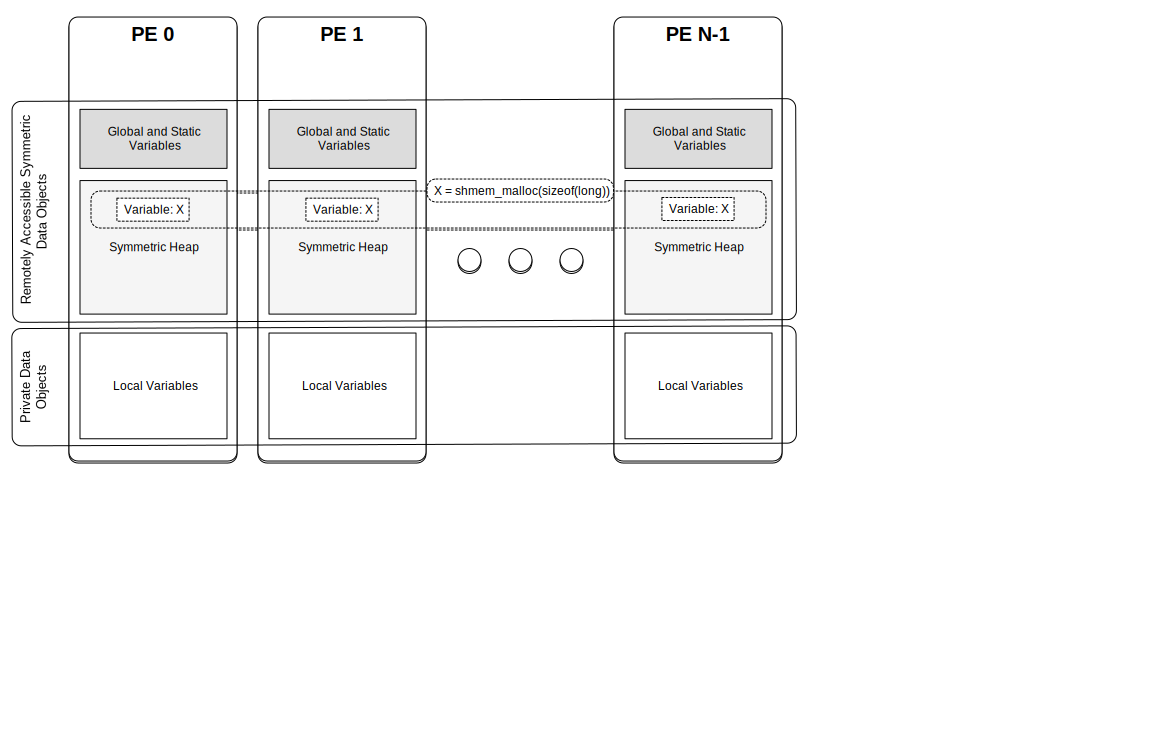
\includegraphics[width=0.95\textwidth]{figures/mem_model}      
\caption{\openshmem Memory Model}
\label{fig:mem_model}                                               
\end{figure}      
%
An \openshmem program consists of data objects that are private to each \ac{PE}
and data  objects that are remotely accessible by all \acp{PE}. Private data
objects are stored in the local memory of each \ac{PE} and can only be accessed
by the \ac{PE} itself; these data objects cannot be accessed by other \acp{PE}
via \openshmem routines. Private data objects follow the memory model of
\Cstd or \Fortran. Remotely accessible objects, however, can be accessed by
remote \acp{PE} using \openshmem routines.  Remotely accessible data objects are
called \emph{Symmetric Data Objects}.  Each symmetric data object has a
corresponding object with the same name, type, and size on all \acp{PE} where that object is
accessible via the \openshmem \ac{API}\footnote{For efficiency reasons,
the same offset (from an arbitrary memory address) for symmetric data
objects might be used on all \acp{PE}. Further discussion about symmetric heap
layout and implementation efficiency can be found in section
\ref{subsec:shfree}}.  (For the definition of what is accessible, see the
descriptions for \FUNC{shmem\_pe\_accessible} and \FUNC{shmem\_addr\_accessible}
in sections \ref{subsec:shmem_pe_accessible} and
\ref{subsec:shmem_addr_accessible}.) Symmetric data objects accessed via typed and
type-generic \openshmem interfaces are required to be naturally aligned based on their type
requirements and underlying architecture.  In \openshmem the following kinds of
data objects are symmetric:
%
\begin{itemize}
\item
  \begin{deprecate}
    \Fortran data objects in common blocks or with the \CTYPE{SAVE} attribute.
    These data objects must not be defined in a dynamic shared object (DSO).
  \end{deprecate}
\item Global and static \Cstd and \Cpp variables. These data objects must
  not  be defined in a DSO.
\item
  \begin{deprecate}
    \Fortran arrays allocated with \FUNC{shpalloc}
  \end{deprecate}
\item \Cstd and \Cpp data allocated by \openshmem memory management routines
  (Section~\ref{sec:memory_management})
\end{itemize}       

\openshmem dynamic memory allocation routines (\FUNC{shpalloc} and
\FUNC{shmem\_malloc}) allow collective allocation of \emph{Symmetric Data
Objects} on a special memory region called the \emph{Symmetric Heap}. The
Symmetric Heap is created during the execution of a program at a memory location
determined by the implementation. The Symmetric Heap may reside in different
memory regions on different \acp{PE}. Figure~\ref{fig:mem_model} shows how
\openshmem implements a \ac{PGAS} model using remotely accessible symmetric
objects and private data objects when executing an \openshmem program.
Symmetric data objects are stored on the symmetric heap or in the global/static
memory section of each \ac{PE}. 

\subsection{Atomicity Guarantees}\label{subsec:amo_guarantees}

\openshmem contains a number of routines that perform atomic operations on
symmetric data objects (Section \ref{sec:amo}).  These routines guarantee that
concurrent accesses to the same location by \openshmem atomic operations using
the same datatype will be exclusive.  However, they do not guarantee
exclusivity when concurrent accesses to the same location are performed using
\openshmem atomic operations using different datatypes, when non-atomic
\openshmem operations are used to access the given location, or when
non-\openshmem operations are performed on the given location.  The result in
such scenarios is undefined.

For example: during the execution of an atomic remote integer increment
operation on a symmetric variable \VAR{X}, no other \openshmem atomic operation
may access \VAR{X}.  After the increment, \VAR{X} will have increased its value
by \CONST{1} on the destination \ac{PE}, at which point other atomic operations
may then modify that \VAR{X}.  However, access to the symmetric object \VAR{X}
with non-atomic operations, such as one-sided \OPR{put} or \OPR{get} operations,
will invalidate the atomicity guarantees.


\section{Execution Model}\label{subsec:execution_model}
An \openshmem program consists of a set of \openshmem processes called \ac{PE}s
that execute in a \ac{SPMD}-like model where each \ac{PE} can take a different
execution path. For example, a \ac{PE} can be implemented using an OS
process.  The \ac{PE}s progress asynchronously, and can communicate/synchronize
via the \openshmem interfaces.  All \ac{PE}s in an \openshmem program should
start by calling the initialization routine  \FUNC{shmem\_init}
\footnote{\textbf{start\_pes} has been deprecated as of Specification 1.2}
before using any of the other \openshmem library routines.  An \openshmem
program finishes execution by returning from the main routine or when any PE
calls \FUNC{shmem\_global\_exit}. When returning from main, \openshmem must
complete all pending communication and release all the resources associated to
the library using an implicit collective synchronization across PEs. The user
has the option to call \FUNC{shmem\_finalize} (before returning from main) to
complete all pending communication and release all the \openshmem library
resources without terminating the program. Calling any \openshmem routine after
\FUNC{shmem\_finalize} leads to undefined behavior.

The \ac{PE}s of the \openshmem program are identified by unique integers.  The
identifiers are integers assigned in a monotonically increasing manner from zero
to the total number of \ac{PE}s minus 1. \ac{PE} identifiers are used for
\openshmem calls (e.g. to specify \OPR{put} or \OPR{get} routines on symmetric
data objects, collective synchronization calls) or to dictate a control flow for
\ac{PE}s using constructs of \Clang{} or \Fortran. The identifiers are fixed for
the life of the \openshmem program.

\subsection{Progress of \openshmem Operations}\label{subsec:progress}

The \openshmem model assumes that computation and communication are naturally
overlapped. \openshmem programs are expected to exhibit progression of
communication both with and without \openshmem calls. Consider a \ac{PE} that is
engaged in a computation with no \openshmem calls. Other \ac{PE}s should be able
to communicate (\OPR{put}, \OPR{get}, \OPR{collective}, \OPR{atomic}, etc) and
complete communication operations with that computationally-bound \ac{PE}
without that \ac{PE} issuing any explicit \openshmem calls. \openshmem
communication calls involving that \ac{PE} should progress regardless of when
that \ac{PE} next engages in an \openshmem call.

\textbf{Note to implementors:}
\begin{itemize}
  \item An \openshmem implementation for hardware that does not provide
      asynchronous communication capabilities may require a software progress
      thread in order to process remotely-issued communication requests without
      explicit program calls to the \openshmem library.  
  \item High performance implementations of \openshmem are expected to leverage
      hardware offload capabilities and provide asynchronous one-sided
      communication without software assistance.
  \item Implementations should avoid deferring the execution of one-sided
      operations until a synchronization point where data is known to be
      available. High-quality implementations should attempt asynchronous delivery
      whenever possible, for performance reasons. Additionally, the \openshmem
      community discourages releasing \openshmem implementations that do not
      provide asynchronous one-sided operations, as these have very limited
      performance value for \openshmem programs.
\end{itemize}

\subsection{Atomicity Guarantees}\label{sec:amo_guarantees}

\openshmem contains a number of routines that operate on symmetric data
atomically (Section \ref{sec:amo}).  These routines guarantee that accesses by
\openshmem's atomic operations with the same datatype will be exclusive, but do not guarantee
exclusivity in combination with other routines, either inside \openshmem or
outside.

For example: during the execution of an atomic remote integer increment
operation on a symmetric variable \VAR{X}, no other \openshmem atomic operation
may access \VAR{X}.  After the increment, \VAR{X} will have increased its value
by \CONST{1} on the destination \ac{PE}, at which point other atomic operations
may then modify that \VAR{X}.  However, access to the symmetric object \VAR{X}
with non-atomic operations, such as one-sided \OPR{put} or \OPR{get} operations,
will \OPR{invalidate} the atomicity guarantees.


\section{Language Bindings and Conformance}\label{subsec:bindings}
\openshmem provides ISO \Cstd language bindings. Any implementation that
provides \Cstd bindings can claim conformance to the specification. The
\openshmem header file \HEADER{shmem.h} for \Cstd must contain only the
interfaces and constant names defined in this specification.

\openshmem \acp{API} can be implemented as either routines or macros. However,
implementing the interfaces using macros is strongly discouraged as this could
severely limit the use of external profiling tools and high-level compiler
optimizations. An \openshmem program should avoid defining routine names,
variables, or identifiers with the prefix \shmemprefix, \shmemprefixC, or with
\openshmem \ac{API} names.

All \openshmem extension \acp{API} that are not part of this specification must
be defined in the \HEADER{shmemx.h} include file for language bindings. This
header file must exist, even if no extensions are provided. Any extensions
shall use the \FUNC{shmemx\_} prefix for all routine, variable, and constant
names.


\section{Library Constants}\label{subsec:library_constants}
\TableIndex{Library Constants}
\TableIndex{Constants}

The \openshmem library provides a set of compile-time constants that may
be used to specify options to API routines, provide implementation-specific
parameters, or return information about the implementation.
All constants that start with \CONST{\_SHMEM\_*} are deprecated,
but provided for backwards compatibility.

\begin{longtable}{|p{0.45\textwidth}|p{0.5\textwidth}|}
\hline
\textbf{Constant} & \textbf{Description}
\tabularnewline \hline
\endhead
%%
\LibConstDecl{SHMEM\_THREAD\_SINGLE} &
The \openshmem thread support level which specifies that the program
must not be multithreaded.
See Section~\ref{subsec:thread_support} for more detail about its use.
\tabularnewline \hline
%%
\LibConstDecl{SHMEM\_THREAD\_FUNNELED} &
The \openshmem thread support level which specifies that the program
may be multithreaded but must ensure that only the main thread invokes
the \openshmem interfaces.
See Section~\ref{subsec:thread_support} for more detail about its use.
\tabularnewline \hline
%%
\LibConstDecl{SHMEM\_THREAD\_SERIALIZED} &
The \openshmem thread support level which specifies that the program
may be multithreaded but must ensure that the \openshmem interfaces
are not invoked concurrently by multiple threads.
See Section~\ref{subsec:thread_support} for more detail about its use.
\tabularnewline \hline
%%
\LibConstDecl{SHMEM\_THREAD\_MULTIPLE} &
The \openshmem thread support level which specifies that the program
may be multithreaded and any thread may invoke the \openshmem interfaces.
See Section~\ref{subsec:thread_support} for more detail about its use.
\tabularnewline \hline
%%
\color{Green}
\LibConstDecl{SHMEM\_TEAM\_NUM\_CONTEXTS} &
\color{Green}
The bitwise flag which specifies that a team creation routine should use the
\VAR{num\_contexts} member of the provided
\CTYPE{shmem\_team\_config\_t} configuration parameter as a request.
See Sections~\ref{subsec:shmem_team_config_t} and
\ref{subsec:shmem_team_split_strided} for more detail about its use.
\tabularnewline \hline
%%
\color{Green}
\LibConstDecl{SHMEM\_TEAM\_NULL} &
\color{Green}
Predefined constant that can be compared against handles of type
\CTYPE{shmem\_team\_t} to determine if they refer to a valid team.
See Section~\ref{subsec:team} for more detail about its use.
\tabularnewline \hline
%%
\LibConstDecl{SHMEM\_CTX\_INVALID} &
A value corresponding to an invalid communication context.
This value can be used to initialize or update context handles to indicate
that they do not reference a valid context.
When managed in this way, applications can use an equality comparison
to test whether a given context handle references a valid context.
See Section~\ref{sec:ctx} for more detail about its use.
\tabularnewline \hline
%%
\LibConstDecl{SHMEM\_CTX\_SERIALIZED} &
The context creation option which specifies that the given context
is shareable but will not be used by multiple threads concurrently.
See Section~\ref{subsec:shmem_ctx_create} for more detail about its use.
\tabularnewline \hline
%%
\LibConstDecl{SHMEM\_CTX\_PRIVATE} &
The context creation option which specifies that the given context
will be used only by the thread that created it.
See Section~\ref{subsec:shmem_ctx_create} for more detail about its use.
\tabularnewline \hline
%%
\LibConstDecl{SHMEM\_CTX\_NOSTORE} &
The context creation option which specifies that quiet and fence operations
performed on the given context are not required to enforce completion and
ordering of memory store operations.
See Section~\ref{subsec:shmem_ctx_create} for more detail about its use.
\tabularnewline \hline
%%
\LibConstDecl{SHMEM\_SYNC\_VALUE}
\begin{DeprecateBlock}
  \LibConstDecl{\_SHMEM\_SYNC\_VALUE}
  \LibConstDecl[\Fortran]{SHMEM\_SYNC\_VALUE}
\end{DeprecateBlock}
&
The value used to initialize the elements of \VAR{pSync} arrays.
The value of this constant is implementation specific.
See Section~\ref{subsec:coll} for more detail about its use.
\tabularnewline \hline
%%
\LibConstDecl{SHMEM\_SYNC\_SIZE}
\begin{DeprecateBlock}
  \LibConstDecl[\Fortran]{SHMEM\_SYNC\_SIZE}
\end{DeprecateBlock}
&
Length of a work array that can be used with any SHMEM collective
communication operation.
Work arrays sized for specific operations may consume less memory.
The value of this constant is implementation specific.
See Section~\ref{subsec:coll} for more detail about its use.
\tabularnewline \hline
%%
\LibConstDecl{SHMEM\_BCAST\_SYNC\_SIZE}
\begin{DeprecateBlock}
  \LibConstDecl{\_SHMEM\_BCAST\_SYNC\_SIZE}
  \LibConstDecl[\Fortran]{SHMEM\_BCAST\_SYNC\_SIZE}
\end{DeprecateBlock}
&
Length of the \VAR{pSync} arrays needed for broadcast routines. The value
of this constant is implementation specific.
See Section~\ref{subsec:shmem_broadcast} for more detail about its use.
\tabularnewline \hline
%%
\LibConstDecl{SHMEM\_REDUCE\_SYNC\_SIZE}
\begin{DeprecateBlock}
  \LibConstDecl{\_SHMEM\_REDUCE\_SYNC\_SIZE}
  \LibConstDecl[\Fortran]{SHMEM\_REDUCE\_SYNC\_SIZE}
\end{DeprecateBlock}
&
Length of the work arrays needed for reduction routines.
The value of this constant is implementation specific.
See Section~\ref{subsec:shmem_reductions} for more detail about its use.
\tabularnewline \hline
%%
\LibConstDecl{SHMEM\_BARRIER\_SYNC\_SIZE}
\begin{DeprecateBlock}
  \LibConstDecl{\_SHMEM\_BARRIER\_SYNC\_SIZE}
  \LibConstDecl[\Fortran]{SHMEM\_BARRIER\_SYNC\_SIZE}
\end{DeprecateBlock}
&
Length of the work array needed for barrier routines.
The value of this constant is implementation specific.
See Section~\ref{subsec:shmem_barrier} for more detail about its use.

\tabularnewline \hline
%%
\LibConstDecl{SHMEM\_COLLECT\_SYNC\_SIZE}
\begin{DeprecateBlock}
  \LibConstDecl{\_SHMEM\_COLLECT\_SYNC\_SIZE}
  \LibConstDecl[\Fortran]{SHMEM\_COLLECT\_SYNC\_SIZE}
\end{DeprecateBlock}
&
Length of the work array needed for collect routines.
The value of this constant is implementation specific.
See Section~\ref{subsec:shmem_collect} for more detail about its use.
\tabularnewline \hline
%%
\LibConstDecl{SHMEM\_ALLTOALL\_SYNC\_SIZE}
\begin{DeprecateBlock}
  \LibConstDecl[\Fortran]{SHMEM\_ALLTOALL\_SYNC\_SIZE}
\end{DeprecateBlock}
&
Length of the work array needed for \FUNC{shmem\_alltoall} routines.
The value of this constant is implementation specific.
See Section~\ref{subsec:shmem_alltoall} for more detail about its use.
\tabularnewline \hline
%%
\LibConstDecl{SHMEM\_ALLTOALLS\_SYNC\_SIZE}
\begin{DeprecateBlock}
  \LibConstDecl[\Fortran]{SHMEM\_ALLTOALLS\_SYNC\_SIZE}
\end{DeprecateBlock}
&
Length of the work array needed for \FUNC{shmem\_alltoalls} routines.
The value of this constant is implementation specific.
See Section~\ref{subsec:shmem_alltoalls} for more detail about its use.
\tabularnewline \hline
%%
\LibConstDecl{SHMEM\_REDUCE\_MIN\_WRKDATA\_SIZE}
\begin{DeprecateBlock}
  \LibConstDecl{\_SHMEM\_REDUCE\_MIN\_WRKDATA\_SIZE}
  \LibConstDecl[\Fortran]{SHMEM\_REDUCE\_MIN\_WRKDATA\_SIZE}
\end{DeprecateBlock}
&
Minimum length of work arrays used in various collective routines.
\tabularnewline \hline
%%
\LibConstDecl{SHMEM\_MAJOR\_VERSION}
\begin{DeprecateBlock}
  \LibConstDecl{\_SHMEM\_MAJOR\_VERSION}
  \LibConstDecl[\Fortran]{SHMEM\_MAJOR\_VERSION}
\end{DeprecateBlock}
&
Integer representing the major version of \openshmem Specification in use.
\tabularnewline \hline
%%
\LibConstDecl{SHMEM\_MINOR\_VERSION}
\begin{DeprecateBlock}
  \LibConstDecl{\_SHMEM\_MINOR\_VERSION}
  \LibConstDecl[\Fortran]{SHMEM\_MINOR\_VERSION}
\end{DeprecateBlock}
&
Integer representing the minor version of \openshmem Specification in use.
\tabularnewline \hline
%%
\LibConstDecl{SHMEM\_MAX\_NAME\_LEN}
\begin{DeprecateBlock}
  \LibConstDecl{\_SHMEM\_MAX\_NAME\_LEN}
  \LibConstDecl[\Fortran]{SHMEM\_MAX\_NAME\_LEN}
\end{DeprecateBlock}
&
Integer representing the maximum length of \CONST{SHMEM\_VENDOR\_STRING}.
\tabularnewline \hline
%%
\LibConstDecl{SHMEM\_VENDOR\_STRING}
\begin{DeprecateBlock}
  \LibConstDecl{\_SHMEM\_VENDOR\_STRING}
  \LibConstDecl[\Fortran]{SHMEM\_VENDOR\_STRING}
\end{DeprecateBlock}
&
String representing vendor defined information of size at most
\CONST{SHMEM\_MAX\_NAME\_LEN}.
In \CorCpp{}, the string is terminated by a null character.  In \Fortran, the
string of size less than \CONST{SHMEM\_MAX\_NAME\_LEN} is padded with blank
characters up to size \CONST{SHMEM\_MAX\_NAME\_LEN}.
\tabularnewline \hline
%%
\LibConstDecl{SHMEM\_CMP\_EQ}
\begin{DeprecateBlock}
  \LibConstDecl{\_SHMEM\_CMP\_EQ}
  \LibConstDecl[\Fortran]{SHMEM\_CMP\_EQ}
\end{DeprecateBlock}
&
An integer constant expression corresponding to the
``equal to'' comparison operation.
See Section~\ref{subsec:p2p_intro} for more detail about its use.
\tabularnewline \hline
%%
\LibConstDecl{SHMEM\_CMP\_NE}
\begin{DeprecateBlock}
  \LibConstDecl{\_SHMEM\_CMP\_NE}
  \LibConstDecl[\Fortran]{SHMEM\_CMP\_NE}
\end{DeprecateBlock}
&
An integer constant expression corresponding to the
``not equal to'' comparison operation.
See Section~\ref{subsec:p2p_intro} for more detail about its use.
\tabularnewline \hline
%%
\LibConstDecl{SHMEM\_CMP\_LT}
\begin{DeprecateBlock}
  \LibConstDecl{\_SHMEM\_CMP\_LT}
  \LibConstDecl[\Fortran]{SHMEM\_CMP\_LT}
\end{DeprecateBlock}
&
An integer constant expression corresponding to the
``less than'' comparison operation.
See Section~\ref{subsec:p2p_intro} for more detail about its use.
\tabularnewline \hline
%%
\LibConstDecl{SHMEM\_CMP\_LE}
\begin{DeprecateBlock}
  \LibConstDecl{\_SHMEM\_CMP\_LE}
  \LibConstDecl[\Fortran]{SHMEM\_CMP\_LE}
\end{DeprecateBlock}
&
An integer constant expression corresponding to the
``less than or equal to'' comparison operation.
See Section~\ref{subsec:p2p_intro} for more detail about its use.
\tabularnewline \hline
%%
\LibConstDecl{SHMEM\_CMP\_GT}
\begin{DeprecateBlock}
  \LibConstDecl{\_SHMEM\_CMP\_GT}
  \LibConstDecl[\Fortran]{SHMEM\_CMP\_GT}
\end{DeprecateBlock}
&
An integer constant expression corresponding to the
``greater than'' comparison operation.
See Section~\ref{subsec:p2p_intro} for more detail about its use.
\tabularnewline \hline
%%
\LibConstDecl{SHMEM\_CMP\_GE}
\begin{DeprecateBlock}
  \LibConstDecl{\_SHMEM\_CMP\_GE}
  \LibConstDecl[\Fortran]{SHMEM\_CMP\_GE}
\end{DeprecateBlock}
&
An integer constant expression corresponding to the
``greater than or equal to'' comparison operation.
See Section~\ref{subsec:p2p_intro} for more detail about its use.
\tabularnewline \hline
%%
\end{longtable}


\section{Library Handles}\label{subsec:library_handles}
\TableIndex{Library Handles}
\TableIndex{Handles}

The \openshmem library provides a set of predefined named constant handles.
All named constants can be used in initialization expressions or assignments,
but not necessarily in array declarations or as labels in \Cstd switch statements.
This implies named constants to be link-time but not necessarily compile-time
constants.

\begin{longtable}{|p{0.45\textwidth}|p{0.5\textwidth}|}
\hline
\textbf{Handle} & \textbf{Description}
\tabularnewline \hline
\endhead
%%
\LibHandleDecl{SHMEM\_TEAM\_WORLD} &
Handle of type \CTYPE{shmem\_team\_t} that corresponds to the
default team of all \acp{PE} in the \openshmem program.  All point-to-point
communication operations and collective synchronizations that do not specify a team
are performed on the default team.
See Section~\ref{subsec:team} for more detail about its use.
\tabularnewline \hline
%%
\LibHandleDecl{SHMEM\_TEAM\_SHARED} &
Handle of type \CTYPE{shmem\_team\_t} that corresponds to a team of \acp{PE}
that share a memory domain.  \LibHandleRef{SHMEM\_TEAM\_SHARED} refers to
the team of all PEs that would mutually return a non-null address from a
call to \FUNC{shmem\_ptr} for all symmetric heap objects.  That is,
\FUNC{shmem\_ptr} must return a non-null pointer to the local PE for all
symmetric heap objects on all target \acp{PE} in the team.  This means that
symmetric heap objects on each \ac{PE} are
directly load/store accessible by all \acp{PE} in the team.
See Section~\ref{subsec:team} for more detail about its use.
\tabularnewline \hline
%%
\LibHandleDecl{SHMEM\_CTX\_DEFAULT} &
Handle of type \CTYPE{shmem\_ctx\_t} that corresponds to the
default communication context.  All point-to-point communication operations
and synchronizations that do not specify a context are performed on the
default context.
See Section~\ref{sec:ctx} for more detail about its use.
\tabularnewline \hline
%%
\end{longtable}


\section{Environment Variables }\label{subsec:environment_variables}
The \openshmem specification provides a set of environment variables that allows
users to configure the \openshmem implementation, and receive information about
the implementation. The implementations of the specification are free to define
additional variables. Currently, the specification defines four environment
variables. All environment variables that start with \VAR{SMA\_*} are
deprecated, but currently supported for backwards compatibility.

\medskip{}

\begin{tabular}{|l|l|l|}
\hline 
Variable & Value & Purpose\tabularnewline
\hline 
\hline 
\texttt{SHMEM\_VERSION} & any & print the library version at
start-up\tabularnewline
\hline 
\texttt{SHMEM\_INFO} & any & print helpful text about all these environment
variables\tabularnewline
\hline 
\texttt{SHMEM\_SYMMETRIC\_SIZE} & non-negative integer & number of bytes to
allocate for symmetric heap\tabularnewline
\hline 
\texttt{SHMEM\_DEBUG} & any & enable debugging messages\tabularnewline
\hline 
\end{tabular}

\medskip{}





\clearpage



\section{OpenSHMEM Library API}\label{sec:openshmem_library_api}

\subsection{Library Setup, Exit, and Query Routines}
The library setup and query interfaces that initialize and monitor the parallel
environment of the \acp{PE}.

\subsubsection{\textbf{SHMEM\_INIT}}\label{subsec:shmem_init}
\apisummary{
    A collective operation that allocates and initializes the resources used by
    the \openshmem library.
}

\begin{apidefinition}

\begin{Csynopsis}
void @\FuncDecl{shmem\_init}@(void);
\end{Csynopsis}

\begin{apiarguments}
    \apiargument{None.}{}{}
\end{apiarguments}

\apidescription{
    \FUNC{shmem\_init} allocates and initializes resources used by the \openshmem
    library. It is a collective operation that all \acp{PE} must call before any
    other \openshmem routine may be called, except \FUNC{shmem\_query\_initialized} 
    which checks the current initialized state of the library. At the end of the 
    \openshmem program which it initialized, the call to \FUNC{shmem\_init} must 
    be matched with a call to \FUNC{shmem\_finalize}.

    The \FUNC{shmem\_init} and \FUNC{shmem\_init\_thread} initialization
    routines may be called multiple times within an \openshmem program. A
    corresponding call to \FUNC{shmem\_finalize} must be made for each call to
    an \openshmem initialization routine. The \openshmem library must not be
    finalized until after the last call to \FUNC{shmem\_finalize} and may be
    re-initialized with a subsequent call to an initialization routine.

}

\apireturnvalues{
    None.
}

\begin{DeprecateBlock}
\apinotes{
    As of \openshmem[1.2], the use of \FUNC{start\_pes} has been
    deprecated and calls to it should be replaced with calls to \FUNC{shmem\_init}.
    While support for \FUNC{start\_pes} is still required in \openshmem libraries,
    users are encouraged to use \FUNC{shmem\_init}. An important difference between
    \FUNC{shmem\_init} and \FUNC{start\_pes} is that every call to
    \FUNC{shmem\_init} within a program must be matched with a call to \FUNC{shmem\_finalize}.
    In the case of \FUNC{start\_pes}, any subsequent calls to \FUNC{start\_pes} after the
    first one results in a no-op.
}
\end{DeprecateBlock}

\begin{apiexamples}

\apicexample
    {The following \FUNC{shmem\_init} example is for \Cstd[11] programs:}
    {example_code/shmem_init_example.c}
    {}

\end{apiexamples}

\end{apidefinition}


\subsubsection{\textbf{SHMEM\_MY\_PE}}\label{subsec:shmem_my_pe}
\apisummary{
    Returns the number of the calling \ac{PE}.
}

\begin{apidefinition}

\begin{Csynopsis}
int shmem_my_pe(void);
\end{Csynopsis}

\begin{Fsynopsis}
INTEGER SHMEM_MY_PE, ME
ME = SHMEM_MY_PE()
\end{Fsynopsis}

\begin{apiarguments}
    \apiargument{None.}{}{}
\end{apiarguments}

\apidescription{
    This routine returns the \ac{PE} number of the calling \ac{PE}.  It accepts no
    arguments.  The result is an integer between \CONST{0} and \VAR{npes} -
    \CONST{1}, where \VAR{npes} is the total number of \ac{PE}s executing the
    current program.
}

\apireturnvalues{
    Integer - Between \CONST{0} and \VAR{npes} - \CONST{1}
}

\apinotes{
    Each \ac{PE} has a unique number or identifier. As of \openshmem Specification
    1.2 the use of \FUNC{\_my\_pe} has been deprecated. Although \openshmem
    libraries are required to support the call, users are encouraged to use
    \FUNC{shmem\_my\_pe} instead.  The behavior and signature  of the routine
    \FUNC{shmem\_my\_pe} remains unchanged from the deprecated \FUNC{\_my\_pe}
    version.
}

\end{apidefinition}


\subsubsection{\textbf{SHMEM\_N\_PES}}\label{subsec:shmem_n_pes}
\apisummary{
    Returns the number of \ac{PE}s running in a program.
}

\begin{apidefinition}

\begin{Csynopsis}
int shmem_n_pes(void);
\end{Csynopsis}

\begin{Fsynopsis}
INTEGER SHMEM_N_PES, N_PES
N_PES = SHMEM_N_PES()
N_PES = NUM_PES()
\end{Fsynopsis}

\begin{apiarguments}
    \apiargument{None.}{}{}
\end{apiarguments}

\apidescription{
    The routine returns the number of \ac{PE}s running the program.
}

\apireturnvalues{
    Integer -  Number of \ac{PE}s running the \openshmem program.
}

\apinotes{
    As of \openshmem Specification 1.2 the use of \FUNC{\_num\_pes} has been
    deprecated. Although \openshmem libraries are required to support the call,
    users are encouraged to use \FUNC{shmem\_n\_pes} instead.
}

\begin{apiexamples}

\apicexample
    {The following \FUNC{shmem\_n\_pes} example is for \CorCpp{} programs:}
    {./example_code/shmem_npes_example.c}
    {}

\end{apiexamples}

\end{apidefinition}


\subsubsection{\textbf{SHMEM\_FINALIZE}}\label{subsec:shmem_finalize}
\apisummary{
    A collective operation that releases all resources used by the \openshmem
    library.  This only terminates the \openshmem portion of a program, not the
    entire program.
}

\begin{apidefinition}

\begin{Csynopsis}
void @\FuncDecl{shmem\_finalize}@(void);
\end{Csynopsis}

\begin{apiarguments}
    \apiargument{None.}{}{}
\end{apiarguments}

\apidescription{
    \FUNC{shmem\_finalize} is a collective operation that ends the \openshmem
    portion of a program previously initialized by \FUNC{shmem\_init} or \FUNC{shmem\_init\_thread} and
    releases all resources used by the \openshmem library. This collective
    operation requires all \acp{PE} to participate in the call. There is an
    implicit global barrier in \FUNC{shmem\_finalize} to ensure that pending
    communications are completed and that no resources are released until all
    \acp{PE} have entered \FUNC{shmem\_finalize}.
    This routine destroys all shareable contexts.  The user is
    responsible for destroying all contexts with the
    \CONST{SHMEM\_CTX\_PRIVATE} option enabled prior to calling this routine;
    otherwise, the behavior is undefined.
    \FUNC{shmem\_finalize} must be
    the last \openshmem library call encountered in the \openshmem portion of a
    program. A call to \FUNC{shmem\_finalize} will release all resources
    initialized by a corresponding call to \FUNC{shmem\_init} or \FUNC{shmem\_init\_thread}. All processes
    that represent the \acp{PE} will still exist after the
    call to \FUNC{shmem\_finalize} returns, but they will no longer have access
    to resources that have been released.
}

\apireturnvalues{
    None.
}

\apinotes{
    \FUNC{shmem\_finalize} releases all resources used by the \openshmem library
    including the symmetric memory heap and pointers initiated by
    \FUNC{shmem\_ptr}. This collective operation requires all \acp{PE} to
    participate in the call, not just a subset of the \acp{PE}. The
    non-\openshmem portion of a program may continue after a call to
    \FUNC{shmem\_finalize} by all \acp{PE}.
}

\begin{apiexamples}

\apicexample
    {The following finalize example is for \Cstd[11] programs:}
    {./example_code/shmem_finalize_example.c}
    {}

\end{apiexamples}

\end{apidefinition}


\subsubsection{\textbf{SHMEM\_GLOBAL\_EXIT}}\label{subsec:shmem_global_exit}
\apisummary{
    A routine that allows any \ac{PE} to force termination of an entire program.
}

\begin{apidefinition}

\begin{C11synopsis}
_Noreturn void shmem_global_exit(int status);
\end{C11synopsis}

\begin{Csynopsis}
void shmem_global_exit(int status);
\end{Csynopsis}

\begin{Fsynopsis}
INTEGER STATUS
CALL SHMEM_GLOBAL_EXIT(status)
\end{Fsynopsis}

\begin{apiarguments}
    \apiargument{IN}{status}{The exit status from the main program.}
\end{apiarguments}

\apidescription{
    \FUNC{shmem\_global\_exit} is a non-collective routine that allows any one
    \ac{PE} to force termination of an \openshmem program for all \acp{PE},
    passing an exit status to the execution environment. This routine terminates
    the entire program, not just the \openshmem portion.  When any \ac{PE} calls
    \FUNC{shmem\_global\_exit}, it results in the immediate notification to all
    \acp{PE} to terminate.  \FUNC{shmem\_global\_exit} flushes I/O and releases
    resources in accordance with C/C++/Fortran language requirements for normal
    program termination. If more than one \ac{PE} calls
    \FUNC{shmem\_global\_exit}, then the exit status returned to the environment
    shall be one of the values passed to \FUNC{shmem\_global\_exit} as the
    status argument.  There is no return to the caller of
    \FUNC{shmem\_global\_exit}; control is returned from the \openshmem program
    to the execution environment for all \acp{PE}.
}

\apireturnvalues{
    None.
}


\apinotes{ 
    \FUNC{shmem\_global\_exit} may be used in situations where one or more
    \acp{PE} have determined that the program has completed and/or should
    terminate early.  Accordingly, the integer status argument can be used to
    pass any information about the nature of the exit, e.g an encountered error
    or a found solution.  Since \FUNC{shmem\_global\_exit} is a non-collective
    routine, there is no implied synchronization, and all \acp{PE} must
    terminate regardless of their current execution state. While I/O must be
    flushed for standard language I/O calls from C/C++/Fortran, it is
    implementation dependent as to how I/O done by other means (e.g. third
    party I/O libraries) is handled. Similarly, resources are released
    according to C/C++/Fortran standard language requirements, but this may not
    include all resources allocated for the \openshmem program. However, a
    quality implementation will make a best effort to flush all I/O and clean
    up all resources.
}

\begin{apiexamples}

\apicexample
    {}
    {./example_code/shmem_global_exit_example.c}
    {}

\end{apiexamples}

\end{apidefinition}


\subsubsection{\textbf{SHMEM\_PE\_ACCESSIBLE}}\label{subsec:shmem_pe_accessible}
\apisummary{
    Determines whether a \ac{PE} is accessible via \openshmem's data transfer
    routines.
}

\begin{apidefinition}

\begin{Csynopsis}
int shmem_pe_accessible(int pe);
\end{Csynopsis}

\begin{Fsynopsis}
LOGICAL LOG, SHMEM_PE_ACCESSIBLE
INTEGER pe
LOG = SHMEM_PE_ACCESSIBLE(pe)
\end{Fsynopsis}

\begin{apiarguments}
    \apiargument{IN}{pe}{Specific \ac{PE} to be checked for accessibility from
    the local \ac{PE}.}
\end{apiarguments}

\apidescription{
    \FUNC{shmem\_pe\_accessible} is a query routine that indicates whether a
    specified \ac{PE} is accessible via \openshmem from the local \ac{PE}. The
    \FUNC{shmem\_pe\_accessible} routine returns a value indicating whether the remote
    \ac{PE} is a process running from the same executable file as the local
    \ac{PE}, thereby indicating whether full support for symmetric data objects,
    which may reside in either static memory or the symmetric heap, is available.
}

\apireturnvalues{
    \CorCpp: The return value is 1 if the specified \ac{PE} is a valid remote \ac{PE}
    for \openshmem routines; otherwise, it is 0.

    \Fortran: The return value is \CONST{.TRUE.} if the specified \ac{PE} is a valid
    remote \ac{PE} for \openshmem routines; otherwise, it is \CONST{.FALSE.}.
}

\apinotes{
    This routine may be particularly useful for hybrid programming with other
    communication libraries (such as \ac{MPI}) or parallel languages.  For
    example, when an \ac{MPI} job uses \ac{MPMD} mode, multiple executable
    \ac{MPI} programs are executed as part of the same MPI job.  In such cases,
    \openshmem support may only be available between processes running from the
    same executable file.  In addition, some environments may allow a hybrid
    job to span multiple network partitions.  In such scenarios, \openshmem
    support may only be available between \acp{PE} within the same partition.
}

\end{apidefinition}


\subsubsection{\textbf{SHMEM\_ADDR\_ACCESSIBLE}}\label{subsec:shmem_addr_accessible}
\apisummary{
    Determines whether an address is accessible via OpenSHMEM data transfer
    routines from the specified  remote \ac{PE}.
}
\index{SHMEM\_ADDR\_ACCESSIBLE}

\begin{apidefinition}

\begin{Csynopsis}
int shmem_addr_accessible(const void *addr, int pe);
\end{Csynopsis}

\begin{Fsynopsis}
LOGICAL LOG, SHMEM_ADDR_ACCESSIBLE
INTEGER pe
LOG = SHMEM_ADDR_ACCESSIBLE(addr, pe)
\end{Fsynopsis}

\begin{apiarguments}
    \apiargument{IN}{addr}{Data object on the local \ac{PE}.}
    \apiargument{IN}{pe}{Integer id of a remote \ac{PE}.}
\end{apiarguments}

\apidescription{
    \FUNC{shmem\_addr\_accessible} is a query routine that indicates whether a local
    address is accessible via \openshmem routines from the specified remote \ac{PE}. 
    
    This routine verifies that the data object is symmetric and accessible with
    respect to a remote \ac{PE} via \openshmem  data  transfer routines.  The
    specified address \VAR{addr} is a data object on the local \ac{PE}. 
    
    This routine may be particularly useful for hybrid programming with other
    communication libraries (such as \ac{MPI}) or parallel languages.  For
    example, in SGI Altix series systems, for multiple executable MPI programs that
    use \openshmem routines, it is important to note that static memory, such as a
    \Fortran common block or \Cstd global variable, is symmetric between
    processes running from the same executable file, but is not symmetric between
    processes running from different executable files.  Data allocated from the
    symmetric heap (\FUNC{shmem\_malloc} or \FUNC{shpalloc}) is symmetric across the
    same or different executable files.
}

\apireturnvalues{		
    \CorCpp: The  return value is \CONST{1} if \VAR{addr} is a symmetric data object
    and accessible via \openshmem routines from the specified remote \ac{PE};
    otherwise, it is \CONST{0}.
    
    \Fortran: The return value is \CONST{.TRUE.} if \VAR{addr} is a symmetric data
    object and accessible via \openshmem routines from the specified remote \ac{PE};
    otherwise, it is \CONST{.FALSE.}.
}
		
\apinotes{
    None.
}

\end{apidefinition}


\subsubsection{\textbf{SHMEM\_PTR}}\label{subsec:shmem_ptr}
\apisummary{
    Returns a local pointer to a symmetric data object on the specified \ac{PE} in the world team.
}

\begin{apidefinition}

\begin{Csynopsis}
void *@\FuncDecl{shmem\_ptr}@(const void *dest, int pe);
\end{Csynopsis}

\begin{apiarguments}
\apiargument{IN}{dest}{The symmetric address of the remotely accessible data
    object to be referenced.}
\apiargument{IN}{pe}{An integer that indicates the \ac{PE} number on which \dest{} is to
    be accessed.}
\end{apiarguments}

\apidescription{
    \FUNC{shmem\_ptr} returns an address that may be used to directly reference
    \dest{} on the specified \ac{PE} in the world team.  This address can be
    assigned to a pointer.  After that, ordinary loads and stores to \dest{} may
    be performed.  The address returned by \FUNC{shmem\_ptr} is a local address
    to a remotely accessible data object.  Providing this address to an argument
    of an \openshmem routine that requires a symmetric address results in
    undefined behavior.

    The \FUNC{shmem\_ptr} routine can provide efficient means to accomplish
    communication, for example when a sequence of reads and writes to a data
    object on a remote \ac{PE} does not match the access pattern provided in an
    \openshmem data transfer routine like \FUNC{shmem\_put} or
    \FUNC{shmem\_iget}.
}

\apireturnvalues{
    A local pointer to the remotely accessible \dest{} data object is returned
    when it can be accessed using memory loads and stores.  Otherwise, a null
    pointer is returned.
}

\apinotes{
    When calling \FUNC{shmem\_ptr}, \dest{} is the address of the referenced
    symmetric data object on the calling \ac{PE}.
}

\begin{apiexamples}

\apicexample
    {In the following \Cstd[11] example, \ac{PE} 0 uses the \FUNC{shmem\_ptr}
    routine to query a pointer and directly access the \VAR{dest} array on
    \ac{PE} 1:}
    {./example_code/shmem_ptr_example.c}
    {}

\end{apiexamples}

\end{apidefinition}


\subsubsection{\textbf{SHMEM\_INFO\_GET\_VERSION}}\label{subsec:shmem_info_get_version}
\apisummary{
    Returns the major and minor version of the library implementation.
}

\begin{apidefinition}

\begin{Csynopsis}
void @\FuncDecl{shmem\_info\_get\_version}@(int *major, int *minor);
\end{Csynopsis}

\begin{Fsynopsis}
INTEGER MAJOR, MINOR
CALL @\FuncDecl{SHMEM\_INFO\_GET\_VERSION}@(MAJOR, MINOR)
\end{Fsynopsis}

\begin{apiarguments}
    \apiargument{OUT}{major}{The major version of the \openshmem Specification in use.}
    \apiargument{OUT}{minor}{The minor version of the \openshmem Specification in use.}
\end{apiarguments}

\apidescription{
    This routine returns the major and minor version of the \openshmem Specification
    in use.  For a given library implementation, the major and minor version
    returned by these calls are consistent with the library constants
    \CONST{SHMEM\_MAJOR\_VERSION} and \CONST{SHMEM\_MINOR\_VERSION}.
}

\apireturnvalues{
    None.
}

\apinotes{
    None. 
}

\end{apidefinition}


\subsubsection{\textbf{SHMEM\_INFO\_GET\_NAME}}\label{subsec:shmem_info_get_name}
\apisummary{
    This routine returns the vendor defined name string that is consistent
    with the library constant \CONST{SHMEM\_VENDOR\_STRING}.
}

\begin{apidefinition}

\begin{Csynopsis}
void @\FuncDecl{shmem\_info\_get\_name}@(char *name);
\end{Csynopsis}

\begin{Fsynopsis}
CHARACTER *(*)NAME
CALL @\FuncDecl{SHMEM\_INFO\_GET\_NAME}@(NAME)
\end{Fsynopsis}

\begin{apiarguments}
    \apiargument{OUT}{name}{The vendor defined string.}
\end{apiarguments}

\apidescription{
    This routine returns the vendor defined name string of size defined by
    the library constant \CONST{SHMEM\_MAX\_NAME\_LEN}. The program calling
    this function provides the \VAR{name} memory buffer of at least size
    \CONST{SHMEM\_MAX\_NAME\_LEN}. The implementation copies the vendor defined
    string of size at most \CONST{SHMEM\_MAX\_NAME\_LEN} to \VAR{name}. In
    \CorCpp, the string is terminated by a null character.  In \Fortran,
    the string of size less than \CONST{SHMEM\_MAX\_NAME\_LEN} is padded with
    blank characters up to size \CONST{SHMEM\_MAX\_NAME\_LEN}. If the
    \VAR{name} memory buffer is provided with size less than
    \CONST{SHMEM\_MAX\_NAME\_LEN}, behavior is undefined. For a given library
    implementation, the vendor string returned is consistent with the library
    constant \CONST{SHMEM\_VENDOR\_STRING}.
}

\apireturnvalues{ 
    None. 
}

\apinotes{ 
    None. 
}

\end{apidefinition}


\subsubsection{\textbf{START\_PES}}\label{subsec:start_pes}
\apisummary{ 
    Called at the beginning of an \openshmem program to initialize the execution
    environment. (This routine is deprecated and is provided for backwards
    compatibility. Implementations must include it, and the routines should
    function properly while notifying the user about deprecation of its use.)
}

\begin{apidefinition}

\begin{Csynopsis}
void start_pes(int npes);
\end{Csynopsis}

\begin{Fsynopsis}
CALL START_PES(npes)
\end{Fsynopsis}

\begin{apiarguments}
       \apiargument{npes}{Unused}{ Should be set to \CONST{0}.}
\end{apiarguments}

\apidescription{   
     The \FUNC{start\_pes} routine initializes the \openshmem execution
     environment.  An \openshmem program must call \FUNC{start\_pes} before
     calling any other \openshmem routine.
}

\apireturnvalues{
    None.
}

\apinotes{
    If any other \openshmem call occurs before \FUNC{start\_pes}, the
    behavior is undefined.  Although it is recommended to set \VAR{npes} to
    \CONST{0} for \FUNC{start\_pes}, this is not mandated.  The value is ignored.
    Calling \FUNC{start\_pes} more than once has no subsequent
    effect.

    As of \openshmem Specification 1.2 the use of \FUNC{start\_pes} has
    been deprecated. Although \openshmem libraries are required to support the
    call, program users are encouraged to use \FUNC{shmem\_init} instead.
}


\begin{apiexamples}

\apicexample
    { This is a simple program that calls \FUNC{start\_pes}:}
    {./example_code/shmem_startpes_example.f90}
    {} 

\end{apiexamples}

\end{apidefinition}


\subsection{Thread Support}
\label{subsec:thread_support}
This section specifies the interaction between \openshmem{} interfaces and the
user threads, and also describes the routines that can be used for initializing and 
querying the thread environment. There are four levels of threading supported by
the \openshmem{} implementation.
 
\begin{itemize}
\item SHMEM\_THREAD\_SINGLE: The \openshmem{} program may not be multithreaded, 
and all \openshmem{} interfaces are invoked by a single thread. 

\item SHMEM\_THREAD\_FUNNELED: 
The \openshmem{} program may be multithreaded, however, the 
program must ensure that only the main thread invokes the \openshmem{}
interfaces.

\item SHMEM\_THREAD\_SERIALIZED: 
The \openshmem{} program may be multithreaded, however, the 
program must ensure that only one thread invokes the \openshmem{}
interfaces at any given instance i.e., the \openshmem{} interfaces 
are not invoked concurrently by multiple threads.

\item SHMEM\_THREAD\_MULTIPLE: 
The \openshmem{} program may be multithreaded, and any 
thread may invoke the \openshmem{} interfaces.
\end{itemize}


\begin{itemize}[leftmargin=*]

\item
In a multithreaded \openshmem{} program multiple threads may issue \openshmem{}
calls. However, the threads are not separately addressable. 
Any \openshmem{} operation initiated by a thread is considered an action of the
\ac{PE} as a whole.

    \begin{itemize}
    \item
    The symmetric heap and symmetric variables scope
    are not impacted by multiple threads invoking the
    \openshmem{} interfaces, i.e., 
    each \ac{PE} has a single symmetric data segment and symmetric heap that is shared by
    all threads within that \ac{PE}.  For example, a thread invoking a memory allocation
    routine such as \FUNC{shmem\_malloc} 
    allocates memory that is accesible by all threads of the \ac{PE}. 
    The requirement that the same symmetric heap operations must
    be executed by all \acp{PE} in the same order also applies in a threaded
    environment. 

    \item
    The completion of collective operations are not impacted by multiple threads. 
    For example, the \FUNC{shmem\_barrier\_all} is completed when all \acp{PE} enter and
    exit the \FUNC{shmem\_barrier\_all} call, even though only one thread in the \ac{PE} is
    participating in the collective call. 
    \end{itemize}                	

\item In an \openshmem{} implementation supporting SHMEM\_THREAD\_MULTIPLE, 
all \openshmem{} calls are thread-safe, i.e., two concurrently running threads
may make \openshmem{} calls and the outcome will be as if the calls executed in
some order, even if their execution is interleaved.

\item Blocking \openshmem{} calls will block the calling thread only, allowing
other threads to execute, if available. The calling thread will be blocked until the
event on which it is waiting occurs. Once the blocked communication is enabled
and can proceed, then the call will complete and the thread will be marked
runnable, within a finite time. A blocked thread will not prevent progress of
other runnable threads on the same \ac{PE}, and will not prevent them from
executing other \openshmem{} calls. Also, a blocked thread will not prevent the
progress of \openshmem{} calls on other \acp{PE}. 
 
\item
In a multithreaded \openshmem{} program, if multiple threads call the collective
calls, it is the programmer's responsibility to ensure the correct ordering of
collective calls.  The symmetric heap management functions, which are defined to call
\FUNC{shmem\_barrier\_all}(\ref{sec:mem_routines}) before they return 
must be treated as collective operations.

\item
\openshmem{} thread calling \FUNC{shmem\_init} is designated as the main
thread. Multiple threads may not call \FUNC{shmem\_init}. Similarly,
\FUNC{shmem\_finalize} may only be called on the main thread.

\end{itemize} 


\subsubsection{\textbf{SHMEM\_INIT\_THREAD}}
\label{subsec:shmem_init_thread}
\apisummary{
Initializes the \openshmem{} library, similar to \FUNC{shmem\_init}, and in addition
perform the initialization required for thread-safe invocation of \openshmem{} functions.}

\begin{apidefinition}

\begin{Csynopsis}
int shmem_init_thread(int requested, int *provided);
\end{Csynopsis}

\begin{apiarguments}
\apiargument{IN}{requested}  {The thread level support requested by the user.
The correct values are SHMEM\_THREAD\_SINGLE, SHMEM\_THREAD\_FUNNELED,
SHMEM\_THREAD\_SERIALIZED, or SHMEM\_THREAD\_MULTIPLE}
\apiargument{OUT}{provided}{The thread level support provided by the \openshmem{} implementation.}
\end{apiarguments}


\apidescription{
    \FUNC{shmem\_init\_thread}  initializes the \openshmem{} library similar to
    \FUNC{shmem\_init}, and in addition perform the initialization required for
    thread-safe invocation of \openshmem{} functions. The argument
    \VAR{requested} is used to specify the desired level of thread support.
    The function returns the support level provided by the library. There are four 
    levels of threading support.
 
 \begin{itemize}
\item SHMEM\_THREAD\_SINGLE: The \openshmem{} program may not be multithreaded, 
and all \openshmem{} interfaces are invoked by a single thread. 

\item SHMEM\_THREAD\_FUNNELED: 
The \openshmem{} program may be multithreaded, however, the 
program must ensure that only one thread invokes the \openshmem{}
interfaces.

\item SHMEM\_THREAD\_SERIALIZED: 
The \openshmem{} program may be multithreaded, however, the 
program must ensure that only one thread invokes the \openshmem{}
interfaces at any given instance i.e., the \openshmem{} interfaces 
are not invoked concurrently by multiple threads.

\item SHMEM\_THREAD\_MULTIPLE: 
The \openshmem{} program may be multithreaded, and any 
thread may invoke the \openshmem{} interfaces.

\item SHMEM\_THREAD\_UNSUPPORTED: The \openshmem{} specification 
can be implemented without the support for threads, or a model beyond the four
models.
   
\end{itemize}

The function may be used to initialize \openshmem{}, and to initialize the
\openshmem{} library with thread safety, instead of \FUNC{shmem\_init}. The
\FUNC{shmem\_init\_thread}
may not be called multiple times in an \openshmem{} program.
}

\apireturnvalues{    
	NONE
    }

\apinotes{
The \openshmem{} programming model does not recognize individual threads.  Any
\openshmem{} operation initiated by a thread is considered an action of the
\ac{PE} as a whole. Thread-safety should not be activated unless needed.
Activating  thread-safety causes additional overhead even if no additional
threads are created or used.
}		


\end{apidefinition}

 
  


\subsubsection{\textbf{SHMEM\_QUERY\_THREAD}}
\label{subsec:shmem_query_thread}
\apisummary{
Returns the level of thread support provided by the library.}


\begin{apidefinition}

\begin{Csynopsis}
void shmem_query_thread(int *provided);
\end{Csynopsis}

\begin{apiarguments}
\apiargument{OUT}{provided}{The thread level support provided by the \openshmem{} implementation.}
\end{apiarguments}


\apidescription{
The \FUNC{shmem\_query\_thread} call returns the level of thread support
currently being provided. The value returned will be same as \textit{provided}
returned in the SHMEM\_INIT\_THREAD(), if the \openshmem{} library was
initialized by SHMEM\_INIT\_THREAD().
}

\apireturnvalues{    
	NONE
}

\apinotes{
}

\end{apidefinition}

 
  



\subsection{Memory Management Routines}
\label{sec:memory_management}

\openshmem provides a set of \acp{API} for managing the symmetric heap. The
\acp{API} allow one to dynamically allocate, deallocate, reallocate and align
symmetric data objects in the symmetric heap.

\subsubsection{\textbf{SHMEM\_MALLOC, SHMEM\_FREE, SHMEM\_REALLOC, SHMEM\_ALIGN}}\label{subsec:shfree}
\apisummary{
    Collective symmetric heap memory management routines.
}

\begin{apidefinition}

\begin{Csynopsis}
void *@\FuncDecl{shmem\_malloc}@(size_t size);
void @\FuncDecl{shmem\_free}@(void *ptr);
void *@\FuncDecl{shmem\_realloc}@(void *ptr, size_t size);
void *@\FuncDecl{shmem\_align}@(size_t alignment, size_t size);
\end{Csynopsis}

\begin{apiarguments}
    \apiargument{IN}{size}{The size, in bytes, of a block to be
        allocated from the symmetric heap. This argument is of type \CTYPE{size\_t}}
    \apiargument{IN}{ptr}{Pointer to a block within the symmetric heap.}
    \apiargument{IN}{alignment}{Byte alignment of the block allocated from the
        symmetric heap.}
\end{apiarguments}


\apidescription{
    The \FUNC{shmem\_malloc}, \FUNC{shmem\_free}, \FUNC{shmem\_realloc}, and
    \FUNC{shmem\_align} routines are collective operations that require
    participation by all \acp{PE}.

    The \FUNC{shmem\_malloc} routine returns a pointer to a block of at least
    \VAR{size} bytes suitably aligned for any use.  This space is allocated from the
    symmetric heap (in contrast to \FUNC{malloc}, which allocates from the private
    heap).  When \VAR{size} is zero, the \FUNC{shmem\_malloc} routine performs
    no action and returns a null pointer.
    
    The \FUNC{shmem\_align} routine allocates a block in the symmetric heap that has
    a byte alignment specified by the \VAR{alignment} argument.  The value of
    \VAR{alignment} shall be a multiple of \CONST{sizeof(void *)}, that is also
    a power of two.  Otherwise, the behavior is undefined.  When \VAR{size} is
    zero, the \FUNC{shmem\_align} routine performs no action and returns a null
    pointer.
    
    The \FUNC{shmem\_free} routine causes the block to which \VAR{ptr} points to be
    deallocated, that is, made available for further allocation.  If \VAR{ptr} is a
    null pointer, no action is performed.
           
    The \FUNC{shmem\_realloc} routine changes the size of the block to which
    \VAR{ptr} points to the size (in bytes) specified by \VAR{size}.  The contents
    of the block are unchanged up to the lesser of the new and old sizes. If the new
    size is larger, the newly allocated portion of the block is
    uninitialized.  If \VAR{ptr} is a null pointer, the
    \FUNC{shmem\_realloc} routine behaves like the \FUNC{shmem\_malloc} routine for
    the specified size.  If \VAR{size} is \CONST{0} and \VAR{ptr} is not a
    null pointer, the block to which it points is freed. If the space cannot
    be allocated, the block to which \VAR{ptr} points is unchanged.
    
    The \FUNC{shmem\_malloc}, \FUNC{shmem\_align}, \FUNC{shmem\_free}, and \FUNC{shmem\_realloc} routines
    are provided  so that multiple \acp{PE} in a program can allocate symmetric,
    remotely accessible memory blocks.  These memory blocks can then be used with
    \openshmem communication routines.  When no action is performed, these
    routines are not collective and return without performing a barrier.
    Otherwise, each of these routines includes at least one
    call to a procedure that is semantically equivalent to \FUNC{shmem\_barrier\_all}:
    \FUNC{shmem\_malloc} and \FUNC{shmem\_align} call a
    barrier on exit; \FUNC{shmem\_free} calls a barrier on entry; and
    \FUNC{shmem\_realloc} may call barriers on both entry and exit, depending on
    whether an existing allocation is modified and whether new memory is allocated.
    This ensures that all
    \acp{PE} participate in the memory allocation, and that the memory on other
    \acp{PE} can be used as soon as the local \ac{PE} returns.
    The implicit barriers performed by these routines quiet the
    default context.  It is the user's responsibility to ensure that no
    communication operations involving the given memory block are pending on
    other contexts prior to calling
    the \FUNC{shmem\_free} and \FUNC{shmem\_realloc} routines.
    The user is also
    responsible for calling these routines with identical argument(s) on all
    \acp{PE}; if differing \VAR{ptr}, \VAR{size}, or \VAR{alignment} arguments are used, the behavior of the call
    and any subsequent \openshmem calls is undefined.
}

\apireturnvalues{
    The \FUNC{shmem\_malloc} routine returns a pointer to the allocated space;
    otherwise, it returns a null pointer.
    
    The \FUNC{shmem\_free} routine returns no value.
    
    The \FUNC{shmem\_realloc} routine returns a pointer to the allocated space
    (which may have moved); otherwise, it returns a null pointer.
    
    The \FUNC{shmem\_align} routine returns an aligned pointer whose value is a
    multiple of \VAR{alignment}; otherwise, it returns a null pointer.
}

\apinotes{ 
    As of \openshmem[1.2] the use of \FUNC{shmalloc}, \FUNC{shmemalign},
    \FUNC{shfree},  and \FUNC{shrealloc} has been deprecated. Although \openshmem
    libraries are required to support the calls, users are encouraged to use
    \FUNC{shmem\_malloc}, \FUNC{shmem\_align}, \FUNC{shmem\_free}, and
    \FUNC{shmem\_realloc} instead.  The behavior and signature  of the routines
    remains unchanged from the deprecated versions.
    					 
    The total size of the symmetric heap is determined at job startup.  One can
    specify the size of the heap using the \VAR{SHMEM\_SYMMETRIC\_SIZE} environment
    variable (where available).	
    
    The \FUNC{shmem\_malloc}, \FUNC{shmem\_free}, and \FUNC{shmem\_realloc} routines
    differ from the private heap allocation routines in that all \acp{PE} in a
    program must call them (a barrier is used to ensure this).
}		

\apiimpnotes{
    The symmetric heap allocation routines always return a pointer to corresponding
    symmetric objects across all \acp{PE}. The \openshmem specification does not
    require that the virtual addresses are equal across all \acp{PE}. Nevertheless,
    the implementation must avoid costly address translation operations in the
    communication path, including $O(N)$ memory translation tables,
    where $N$ is the number of \acp{PE}.  In order to avoid address translations, the
    implementation may re-map the allocated block of memory based on agreed virtual
    address.  Additionally, some operating systems provide an option to disable
    virtual address randomization, which enables predictable allocation of virtual
    memory addresses.
}

\end{apidefinition}


\subsubsection{\textbf{SHMEM\_CALLOC}}\label{subsec:shmem_calloc}
\apisummary{
  Allocate a zeroed block of symmetric memory.
}
\index{SHMEM\_CALLOC}

\begin{apidefinition}

\begin{Csynopsis}
void *shmem_calloc(size_t count, size_t size);
\end{Csynopsis}

\begin{apiarguments}
  \apiargument{IN}{count}{The number of elements to allocate.}
  \apiargument{IN}{size}{The size in bytes of each element to allocate.}
\end{apiarguments}


\apidescription{
  The \FUNC{shmem\_calloc} routine allocates a region of remotely-accessible
  memory for an array of \VAR{count} objects of \VAR{size} bytes each and
  returns a pointer to the lowest byte address of the allocated symmetric
  memory. The space is initialized to all bits zero.

  If the allocation succeeds, the pointer returned shall be suitably
  aligned so that it may be assigned to a pointer to any type of object.
  If the allocation does not succeed, or either \VAR{count} or \VAR{size} is
  \CONST{0}, the return value is a null pointer.

  The values for \VAR{count} and \VAR{size} shall each be equal across
  all \acp{PE} calling \FUNC{shmem\_calloc}; otherwise, the behavior is
  undefined.

  The \FUNC{shmem\_calloc} routine calls \FUNC{shmem\_barrier\_all} on exit.
}

\apireturnvalues{
  The \FUNC{shmem\_calloc} routine returns a pointer to the lowest byte
  address of the allocated space; otherwise, it returns a null pointer.
}

\apinotes{
  None.
}

\end{apidefinition}


\subsubsection{\textbf{SHPALLOC}}\label{subsec:shpalloc}
\apisummary{
    Allocates a block of memory from the symmetric heap.
}

\begin{apidefinition}

\begin{Fsynopsis}
POINTER (addr, A(1))
INTEGER length, errcode, abort
CALL @\FuncDecl{SHPALLOC}@(addr, length, errcode, abort)
\end{Fsynopsis}

\begin{apiarguments}
    \apiargument{OUT}{addr}{First word address of the allocated block.}
    \apiargument{IN}{length}{Number of words of memory requested. One word is 32 bits.}
    \apiargument{OUT}{errcode}{Error code is \CONST{0} if no error was detected;
    otherwise, it is a negative integer code for the type of error.}
    \apiargument{IN}{abort}{Abort code; nonzero requests abort on error;
    \CONST{0}  requests an error code.}
\end{apiarguments}

\apidescription{   
    \FUNC{SHPALLOC} allocates a block of memory from the program's symmetric heap
    that is greater than or equal to the size requested. To maintain symmetric heap
    consistency, all \acp{PE} in an program must call \FUNC{SHPALLOC} with the same
    value of length; if any  \acp{PE} are missing, the program will hang.
    
    By using the \Fortran \CONST{POINTER} mechanism in the following manner, 
    array \VAR{A} can be used to refer to the block allocated by \FUNC{SHPALLOC}:
    \CONST{POINTER} (\VAR{addr}, \VAR{A}())
}

\apireturnvalues{}
    \apitablerow{Error Code}{Condition}
    \apitablerow{ \CONST{-1} }{Length is not an integer greater than \CONST{0}}
    \apitablerow{\CONST{-2}}{ No more memory is available from the system (checked if the
    request cannot be satisfied from the available blocks on the symmetric heap).}

\apinotes{  
    The total size of the symmetric heap is determined at job startup.  One may
    adjust the size of the heap using the \VAR{SHMEM\_SYMMETRIC\_SIZE} environment
    variable (if available).	
}

\apiimpnotes{
    The symmetric heap allocation routines always return a pointer to corresponding
    symmetric objects across all \acp{PE}. The \openshmem specification does not
    require that the virtual addresses are equal across all \acp{PE}. Nevertheless,
    the implementation must avoid costly address translation operations in the
    communication path, including order $N$ (where $N$ is the number of \acp{PE})
    memory translation tables.  In order to avoid address translations, the
    implementation may re-map the allocated block of memory based on agreed virtual
    address.  Additionally, some operating systems provide an option to disable
    virtual address randomization, which enables predictable allocation of virtual
    memory addresses.
}

\end{apidefinition}


\subsubsection{\textbf{SHPCLMOVE}}\label{subsec:shpclmove}
\apisummary{
    Extends  a symmetric heap block or copies the contents of the block into a
    larger block.
}

\begin{apidefinition}

\begin{Fsynopsis}
POINTER (addr, A(1))
INTEGER length, status, abort
CALL SHPCLMOVE (addr, length, status, abort)
\end{Fsynopsis}

\begin{apiarguments}
    \apiargument{INOUT}{addr}{On  entry, first word address of the block to
    change; on exit, the new address of the block if it was moved.}
    \apiargument{IN}{length}{Requested new total length in words. One word is
    \CONST{32} bits.}
    \apiargument{OUT}{status}{Status is \CONST{0} if the block was extended in
    place, \CONST{1} if it was moved, and a negative integer for the type of
    error detected.}
    \apiargument{IN}{abort}{Abort code.  Nonzero requests abort on error;
    \CONST{0} requests an error code.}
\end{apiarguments}
 
\apidescription{     
    The \FUNC{SHPCLMOVE} routine either extends a symmetric heap block if the block
    is followed by a large enough free block or copies the contents of the existing
    block to a larger block and returns a status code indicating that the block was
    moved.  This routine also can reduce the size of a block if the new length is
    less than  the old length.  All \acp{PE}  in a program must call
    \FUNC{SHPCLMOVE} with the same value of \VAR{addr} to maintain symmetric heap
    consistency; if any \acp{PE} are missing, the program hangs.
}

\apireturnvalues{
    \retvaldesctable{
    \retvaltablerow{\CONST{-1} }{Length is not an integer greater than \CONST{0}}
    \retvaltablerow{\CONST{-2}}{ No more memory is available from the system (checked  if the  request  cannot  be satisfied from the available blocks on the symmetric heap).}
    \retvaltablerow{\CONST{-3}}{Address is outside the bounds of the symmetric heap.}
    \retvaltablerow{\CONST{-4}}{Block is already free.}
    \retvaltablerow{\CONST{-5}}{Address is not at the beginning of a block.}
    }
}

\end{apidefinition}


\subsubsection{\textbf{SHPDEALLC}}\label{subsec:shpdeallc}
       Returns a memory block to the symmetric heap.

SYNOPSIS
       POINTER (addr, A(1))
       INTEGER errcode, abort
       CALL SHPDEALLC(addr, errcode, abort)

DESCRIPTION

Arguments

       IN	addr	      First word address of the block to deallocate.
       OUT	errcode	      Error  code is 0 if no error was detected; otherwise, it
		      is a  negative  integer  code  for  the  type  of	 error.
       IN	abort	      Abort code.  Nonzero requests abort on error; 0 requests
		      an error code.

API Description

       SHPDEALLC  returns  a block of memory (allocated using SHPALLOC) to the
       list of available space in the symmetric heap.  To  maintain  symmetric
       heap  consistency, all processing elements (PEs) in a program must call
       SHPDEALLC with the same value of addr; if  any  PEs  are	 missing,  the
       program hangs.


Return Value

       Error conditions are as follows:

       Code	      Condition
       -3	      Address is outside the bounds of the symmetric heap.
       -4	      Block is already free.
       -5	      Address is not at the beginning of the block.

NOTES



\subsection{Communication Management Routines}
\label{sec:ctx}
All \openshmem RMA, AMO, and memory ordering routines are
performed on a communication context.  The communication context defines an
independent ordering and completion environment, allowing users to manage the
overlap of communication with computation and also to manage communication
operations performed by separate threads within a multithreaded \ac{PE}.  For
example, in single-threaded environments, contexts may be used to pipeline
communication and computation.  In multithreaded environments, contexts may
additionally provide thread isolation, eliminating overheads resulting from
thread interference.

Context handles are of type \CTYPE{shmem\_ctx\_t} and are valid for
language-level assignment and equality comparison.  A handle to the desired context is
passed as an argument in the \Cstd \CTYPE{shmem\_ctx\_*} and type-generic API
routines.  API routines that do not accept a context argument operate on the
default context.  The default context can be used explicitly through the
\LibHandleRef{SHMEM\_CTX\_DEFAULT} handle.

\subsubsection{\textbf{SHMEM\_CTX\_CREATE}}
\label{subsec:shmem_ctx_create}
\apisummary{
    Create a communication context.
}

\begin{apidefinition}

\begin{Csynopsis}
int @\FuncDecl{shmem\_ctx\_create}@(long options, shmem_ctx_t *ctx);
\end{Csynopsis}

\begin{apiarguments}
    \apiargument{IN}{options}{The set of options requested for the given context.
        Multiple options may be requested by combining them with a bitwise
        OR operation; otherwise, \CONST{0} can be given if no options are
        requested.}
    \apiargument{OUT}{ctx}{A handle to the newly created context.}
\end{apiarguments}

\apidescription{
    The \FUNC{shmem\_ctx\_create} routine creates a new communication context
    and returns its handle through the \VAR{ctx} argument.  If the context was
    created successfully, a value of zero is returned
    and the context handle pointed to by \VAR{ctx} specifies a valid context;
    otherwise, a nonzero value is returned and \VAR{ctx} is set to
    \LibConstRef{SHMEM\_CTX\_INVALID}.
    An unsuccessful context
    creation call is not treated as an error and the \openshmem library remains
    in a correct state.  The creation call can be reattempted with different
    options or after additional resources become available.

    A newly created communication context has a fixed association with the
    default team.
    All \openshmem routines that operate on this context will do so with
    respect to the associated \ac{PE} team.
    That is, all point-to-point routines operating on this context will use
    team-relative \ac{PE} numbering.

    By default, contexts are {\em shareable} and, when it is allowed by the
    threading model provided by the \openshmem library, they can be used concurrently by
    multiple threads within the PE where they were created.
    %
    The following options can be supplied during context creation to restrict
    this usage model and enable performance optimizations.  When using a given
    context, the application must comply with the requirements of all options
    set on that context; otherwise, the behavior is undefined.
    No options are enabled on the default context.

        \apitablerow{\LibConstRef{SHMEM\_CTX\_SERIALIZED}}{
            The given context is shareable; however, it will not be used by multiple threads
            concurrently.  When the \CONST{SHMEM\_CTX\_SERIALIZED} option is
            set, the user must ensure that operations involving the given
            context are serialized by the application.}

        \apitablerow{\LibConstRef{SHMEM\_CTX\_PRIVATE}}{
            The given context will be used only by the thread that created it.}

        \apitablerow{\LibConstRef{SHMEM\_CTX\_NOSTORE}}{
            Quiet and fence operations performed on the given context are not
            required to enforce completion and ordering of memory store
            operations.
            When ordering of store operations is needed, the application must
            perform a synchronization operation on a context without the
            \CONST{SHMEM\_CTX\_NOSTORE} option enabled.}

}

\apireturnvalues{
    Zero on success and nonzero otherwise.
}

\apinotes{
    None.
}

\end{apidefinition}



\subsubsection{\textbf{SHMEM\_CTX\_DESTROY}}
\label{subsec:shmem_ctx_destroy}
\apisummary{
    Destroy a \newtext{locally created} communication context.
}

\begin{apidefinition}

\begin{Csynopsis}
void @\FuncDecl{shmem\_ctx\_destroy}@(shmem_ctx_t ctx);
\end{Csynopsis}

\begin{apiarguments}
    \apiargument{IN}{ctx}{Handle to the context that will be destroyed.}
\end{apiarguments}

\apidescription{
    \FUNC{shmem\_ctx\_destroy} destroys a context that was created by a call to
    \FUNC{shmem\_ctx\_create} \newtext{or \FUNC{shmem\_team\_create\_ctx}}.
    It is the user's responsibility to ensure that
    the context is not used after it has been destroyed, for example when the
    destroyed context is used by multiple threads.  This function
    performs an implicit quiet operation on the given context before it is freed.
    If \VAR{ctx} has the value \CONST{SHMEM\_CTX\_INVALID}, no operation is
    performed.
}

\apireturnvalues{
    None.
}

\apinotes{
    \oldtext{
    It is invalid to pass \CONST{SHMEM\_CTX\_DEFAULT} to this routine.
    }

    Destroying a context makes it impossible for the user to complete
    communication operations that are pending on that context.  This includes
    nonblocking communication operations, whose local buffers are only returned
    to the user after the operations have been completed.  An implicit quiet is
    performed when freeing a context to avoid this ambiguity.

    A context with the \CONST{SHMEM\_CTX\_PRIVATE} option enabled must be
    destroyed by the thread that created it.
}

\begin{apiexamples}

    \apicexample
    {The following example demonstrates the use of contexts in a multithreaded
    \Cstd[11] program that uses OpenMP for threading.  This example shows the
    shared counter load balancing method and illustrates the use of contexts
    for thread isolation.}
    {./example_code/shmem_ctx.c}
    {}

    \apicexample
    {The following example demonstrates the use of contexts in a
    single-threaded \Cstd[11] program that performs a summation reduction where
    the data contained in the \VAR{in\_buf} arrays on all \acp{PE} is reduced into
    the \VAR{out\_buf} arrays on all \acp{PE}.  The buffers are divided into
    segments and processing of the segments is pipelined.  Contexts are used
    to overlap an all-to-all exchange of data for segment \VAR{p} with the
    local reduction of segment \VAR{p-1}.}
    {./example_code/shmem_ctx_pipelined_reduce.c}
    {}

    \apicexample
    {The following example demonstrates the use of \CONST{SHMEM\_CTX\_INVALID}
    in a \Cstd[11] program that uses thread-local storage to provide each
    thread an implicit context handle via a ``library'' put routine without
    explicit management of the context handle from ``user'' code.}
    {./example_code/shmem_ctx_invalid.c}
    {}

\end{apiexamples}

\end{apidefinition}




\subsection{Remote Memory Access Routines}\label{sec:rma}
The \ac{RMA} routines described in this section are one-sided communication
mechanisms of the \openshmem{} \ac{API}. While using these mechanisms, the user
is required to provide parameters only on the calling side. A characteristic of
one-sided communication is that it decouples communication from the
synchronization. One-sided communication mechanisms transfer the data but do not
synchronize the sender of the data with the receiver of the data. 

\openshmem{} \ac{RMA} routines are all performed on the symmetric objects.  The
initiator \ac{PE} of the call is designated as \source{}, and the \ac{PE} in
which memory is accessed is designated as \dest{}. In the case of the remote
update routine, \PUT{}, the origin is the \source{} \ac{PE} and the destination
\ac{PE} is the \dest{} PE. In the case of the remote read routine, \GET{}, the
origin is the \dest{} \ac{PE} and the destination is the \source{} \ac{PE}.

Where appropriate compiler support is available, \openshmem{} provides type-generic 
one-sided communication interfaces via \Celev{}%
\footnote{Formally, the \Celev{} specification is ISO/IEC 9899:2011(E).}
generic selection (\Celev{} \S6.5.1.1)
for block, scalar, and block-strided put and get communication. 
Such type-generic routines are supported for the ``standard \ac{RMA} types''
listed in Table \ref{stdrmatypes}.

% Fix the C99 styling here with the macros from PR #55 and
% osh_spec_next for \HEADER{}
The standard \ac{RMA} types include the exact-width integer types defined in
\textit{stdint.h} by \textit{C99}%
\footnote{Formally, the \textit{C99} specification is ISO/IEC~9899:1999(E).}%
~\S7.18.1.1 and \Celev{}~\S7.20.1.1. When the \Clang{} translation environment
does not provide exact-width integer types with \textit{stdint.h}, an
\openshmem implemementation is not required to provide support for these types.

\begin{table}[h]
  \begin{center}
    \begin{tabular}{|l|l|}
      \hline
      \TYPE              & \TYPENAME  \\ \hline
      float              & float      \\ \hline
      double             & double     \\ \hline
      long double        & longdouble \\ \hline
      char               & char       \\ \hline
      signed char        & schar      \\ \hline
      short              & short      \\ \hline
      int                & int        \\ \hline
      long               & long       \\ \hline
      long long          & longlong   \\ \hline
      unsigned char      & uchar      \\ \hline
      unsigned short     & ushort     \\ \hline
      unsigned int       & uint       \\ \hline
      unsigned long      & ulong      \\ \hline
      unsigned long long & ulonglong  \\ \hline
      int8\_t            & int8       \\ \hline
      int16\_t           & int16      \\ \hline
      int32\_t           & int32      \\ \hline
      int64\_t           & int64      \\ \hline
      uint8\_t           & uint8      \\ \hline
      uint16\_t          & uint16     \\ \hline
      uint32\_t          & uint32     \\ \hline
      uint64\_t          & uint64     \\ \hline
      size\_t            & size       \\ \hline
      ptrdiff\_t         & ptrdiff    \\ \hline
    \end{tabular}
    \caption{Standard \ac{RMA} Types and Names}
    \label{stdrmatypes}
  \end{center} 
\end{table}


\subsubsection{\textbf{SHMEM\_PUT}}\label{subsec:shmem_put}
\apisummary{
    The  put routines  provide  a method for copying data from a contiguous local
    data object to a data object on a specified \ac{PE}.
}

\begin{apidefinition}

\begin{Csynopsis}
void shmem_double_put(double *dest, const double *source, size_t nelems, int pe);
void shmem_float_put(float *dest, const float *source, size_t nelems, int pe);
void shmem_int_put(int *dest, const int *source, size_t nelems, int pe);
void shmem_long_put(long *dest, const long *source, size_t nelems, int pe);
void shmem_longdouble_put(long double *dest, const long double *source, size_t nelems, int pe);
void shmem_longlong_put(long long *dest, const long long *source, size_t nelems, int pe);
void shmem_put32(void *dest, const void *source, size_t nelems, int pe);
void shmem_put64(void *dest, const void *source, size_t nelems, int pe);
void shmem_put128(void *dest, const void *source, size_t nelems, int pe);
void shmem_putmem(void *dest, const void *source, size_t nelems, int pe);
void shmem_short_put(short*dest, const short*source, size_t nelems, int pe);
\end{Csynopsis}

\begin{Fsynopsis}
CALL SHMEM_CHARACTER_PUT(dest, source, nelems, pe)
CALL SHMEM_COMPLEX_PUT(dest, source, nelems, pe)
CALL SHMEM_DOUBLE_PUT(dest, source, nelems, pe)
CALL SHMEM_INTEGER_PUT(dest, source, nelems, pe)
CALL SHMEM_LOGICAL_PUT(dest, source, nelems, pe)
CALL SHMEM_PUT4(dest, source, nelems, pe)
CALL SHMEM_PUT8(dest, source, nelems, pe)
CALL SHMEM_PUT32(dest, source, nelems, pe)
CALL SHMEM_PUT64(dest, source, nelems, pe)
CALL SHMEM_PUT128(dest, source, nelems, pe)
CALL SHMEM_PUTMEM(dest, source, nelems, pe)
CALL SHMEM_REAL_PUT(dest, source, nelems, pe)
\end{Fsynopsis}

\begin{apiarguments}
    \apiargument{IN}{dest}{Data object to be updated on the remote \ac{PE}. This
    data object must be remotely accessible.}
    \apiargument{OUT}{source}{Data object containing the data to be copied.}
    \apiargument{IN}{nelems}{Number of elements in the \VAR{dest} and \VAR{source}
    arrays. \VAR{nelems} must be of type \VAR{size\_t} for \Clang. If you are using
    \Fortran, it must be a constant, variable, or array element of default
    integer type.}
    \apiargument{IN}{pe}{\ac{PE} number of the remote \ac{PE}. \VAR{pe} must be
    of type integer. If you are using \Fortran, it must be a constant, variable,
    or array element of default integer type.}
\end{apiarguments}

\apidescription{
    The routines return after the data has been copied out of the \source{} array
    on the local \ac{PE}.  The delivery of data words into the data object on the
    destination \ac{PE} may occur in any order.  Furthermore, two successive put
    routines may deliver data out of order unless a call to \FUNC{shmem\_fence} is
    introduced between the two calls.   
 }

\apidesctable{
    The \dest{} and \source{} data objects must conform to certain typing
    constraints, which are as follows:}
    {Routine}{Data type of \VAR{dest} and \VAR{source}}
    \apitablerow{shmem\_putmem}{\Fortran: Any noncharacter type. \Clang: Any
        data  type.  nelems is scaled in bytes.}
    \apitablerow{shmem\_put4, shmem\_put32}{Any noncharacter type
        that has a storage size equal to \CONST{32} bits.}
    \apitablerow{shmem\_put8, shmem\_put64}{Any noncharacter type that
        has a storage size equal to \CONST{64} bits.}
    \apitablerow{shmem\_put128}{Any noncharacter type that has a
        storage size equal to \CONST{128} bits.}
    \apitablerow{shmem\_double\_put}{Elements of type double.}
    \apitablerow{shmem\_longdouble\_put}{Elements of type long double.}
    \apitablerow{SHMEM\_CHARACTER\_PUT}{Elements of type character.  \VAR{nelems}
    is  the number  of	 characters to transfer. The actual character lengths of
    the \source{} and \dest{} variables are ignored. }
    \apitablerow{SHMEM\_COMPLEX\_PUT}{Elements of type complex of default size.}
    \apitablerow{SHMEM\_DOUBLE\_PUT}{Elements of type double precision. }
    \apitablerow{SHMEM\_INTEGER\_PUT}{Elements of type integer.}
    \apitablerow{SHMEM\_LOGICAL\_PUT}{Elements of type logical.}
    \apitablerow{SHMEM\_REAL\_PUT}{Elements of type real.}

\apireturnvalues{
    None.
}
\apinotes{
    If you are using \Fortran, data types must be of default size.  For example,
    a real variable must be declared as \CONST{REAL},  \CONST{REAL*4},  or
    \CONST{REAL(KIND=KIND(1.0))}. The Fortran API routine \FUNC{SHMEM\_PUT} has
    been deprecated, and either \FUNC{SHMEM\_PUT8} or \FUNC{SHMEM\_PUT64} should
    be used in its place.
}

\begin{apiexamples}

\apicexample
    { The following \FUNC{shmem\_put} example is for \CorCpp{} programs:}
    {./example_code/shmem_put_example.c}
    {} 
\end{apiexamples}

\end{apidefinition}


\subsubsection{\textbf{SHMEM\_P}}\label{subsec:shmem_p}
\apisummary{
    Copies one data item to a remote \ac{PE}.
}

\begin{apidefinition}

\begin{C11synopsis}
void @\FuncDecl{shmem\_p}@(TYPE *dest, TYPE value, int pe);
void @\FuncDecl{shmem\_p}@(shmem_ctx_t ctx, TYPE *dest, TYPE value, int pe);
\end{C11synopsis}
where \TYPE{} is one of the standard \ac{RMA} types specified by Table \ref{stdrmatypes}.

\begin{Csynopsis}
void @\FuncDecl{shmem\_\FuncParam{TYPENAME}\_p}@(TYPE *dest, TYPE value, int pe);
void @\FuncDecl{shmem\_ctx\_\FuncParam{TYPENAME}\_p}@(shmem_ctx_t ctx, TYPE *dest, TYPE value, int pe);
\end{Csynopsis}
where \TYPE{} is one of the standard \ac{RMA} types and has a corresponding \TYPENAME{} specified by Table \ref{stdrmatypes}.

\begin{apiarguments}
  \apiargument{IN}{ctx}{A context handle specifying the context on which to perform the operation.
    When this argument is not provided, the operation is performed on
    the default context.}
  \apiargument{OUT}{dest}{Symmetric address of the destination data object.
    The type of \dest{} should match that implied in the SYNOPSIS section.}
  \apiargument{IN}{value}{The value to be transferred to \VAR{dest}.
    The type of \VAR{value} should match that implied in the SYNOPSIS section.}
  \apiargument{IN}{pe}{The number of the remote \ac{PE}.}
\end{apiarguments}

\apidescription{
    These routines provide a very low latency put capability for single elements of
    most basic types.
    
    As with \FUNC{shmem\_put}, these routines start the remote transfer and may
    return before the data is delivered to the remote \ac{PE}.  Use
    \FUNC{shmem\_quiet} to force completion of all remote \PUT{} transfers.
}

\apireturnvalues{
    None.
}

\begin{apiexamples}

    \apicexample
    {The following example uses \FUNC{shmem\_p} in a \Cstd[11] program.}
    {./example_code/shmem_p_example.c}
    {}

\end{apiexamples}

\end{apidefinition}


\subsubsection{\textbf{SHMEM\_IPUT}}\label{subsec:shmem_iput}
\apisummary{
    Copies strided data to a specified \ac{PE}.
}

\begin{apidefinition}

\begin{C11synopsis}
void @\FuncDecl{shmem\_iput}@(TYPE *dest, const TYPE *source, ptrdiff_t dst, ptrdiff_t sst, size_t nelems, int pe);
void @\FuncDecl{shmem\_iput}@(shmem_ctx_t ctx, TYPE *dest, const TYPE *source, ptrdiff_t dst, ptrdiff_t sst, size_t nelems, int pe);
\end{C11synopsis}
where \TYPE{} is one of the standard \ac{RMA} types specified by Table \ref{stdrmatypes}.

\begin{Csynopsis}
void @\FuncDecl{shmem\_\FuncParam{TYPENAME}\_iput}@(TYPE *dest, const TYPE *source, ptrdiff_t dst, ptrdiff_t sst, size_t nelems, int pe);
void @\FuncDecl{shmem\_ctx\_\FuncParam{TYPENAME}\_iput}@(shmem_ctx_t ctx, TYPE *dest, const TYPE *source, ptrdiff_t dst, ptrdiff_t sst, size_t nelems, int pe);
\end{Csynopsis}
where \TYPE{} is one of the standard \ac{RMA} types and has a corresponding \TYPENAME{} specified by Table \ref{stdrmatypes}.

\begin{CsynopsisCol}
void @\FuncDecl{shmem\_iput\FuncParam{SIZE}}@(void *dest, const void *source, ptrdiff_t dst, ptrdiff_t sst, size_t nelems, int pe);
void @\FuncDecl{shmem\_ctx\_iput\FuncParam{SIZE}}@(shmem_ctx_t ctx, void *dest, const void *source, ptrdiff_t dst, ptrdiff_t sst, size_t nelems, int pe);
\end{CsynopsisCol}
where \SIZE{} is one of \CONST{8, 16, 32, 64, 128}.

\begin{apiarguments}
    \apiargument{IN}{ctx}{A context handle specifying the context on which to perform the operation.
        When this argument is not provided, the operation is performed on
        the default context.}
    \apiargument{OUT}{dest}{Array to be updated on the remote \ac{PE}. This data
        object  must be remotely accessible.}
    \apiargument{IN}{source}{Array containing the data to be copied.}
    \apiargument{IN}{dst}{The stride between consecutive elements of the \dest{}
        array.  The stride is scaled by the element size of the \dest{} array.  A
        value of \CONST{1} indicates contiguous data.  \VAR{dst} must be of type
        \CTYPE{ptrdiff\_t}.}
    \apiargument{IN}{sst}{The  stride between consecutive elements of the
        \source{} array.  The stride is scaled by the element size of the \source{}
        array.  A  value of \CONST{1} indicates contiguous data.  \VAR{sst} must be
        of type \CTYPE{ptrdiff\_t}.}
    \apiargument{IN}{nelems}{Number of elements in the \dest{} and \source{}
        arrays.  \VAR{nelems} must be of type \VAR{size\_t} for \Cstd.}
    \apiargument{IN}{pe}{\ac{PE} number of the remote \ac{PE}.  \VAR{pe} must be
        of type integer.}
\end{apiarguments}


\apidescription{
    The \FUNC{iput} routines provide a method  for  copying strided data
    elements (specified by \VAR{sst}) of an array from a \source{} array on the
    local \ac{PE} to locations specified by stride \VAR{dst} on a \dest{} array
    on specified remote \ac{PE}. Both strides, \VAR{dst} and \VAR{sst}, must be
    greater than or equal to \CONST{1}. The routines return when the data has
    been copied out of the \VAR{source} array on the local \ac{PE} but not
    necessarily before the data has been delivered to the remote data object.
    If the context handle \VAR{ctx} does not correspond to a valid context,
    the behavior is undefined.
}

\apidesctable{
    The \dest{} and \source{} data objects must conform to typing constraints,
    which are as follows:
}{Routine}{Data type of \VAR{dest} and \VAR{source}}
    \apitablerow{shmem\_iput4, shmem\_iput32}{Any noncharacter type
        that has a storage size equal to \CONST{32} bits.}
    \apitablerow{shmem\_iput8}{\Cstd: Any noncharacter type that
        has a storage size equal to \CONST{8} bits.}
    \apitablerow{shmem\_iput64}{Any noncharacter type that
        has a storage size equal to \CONST{64} bits.}
    \apitablerow{shmem\_iput128}{Any noncharacter type that has a
        storage size equal to \CONST{128} bits.}

\apireturnvalues{
    None.
}

\apinotes{
    See Section \ref{subsec:memory_model} for a definition of the term
    remotely accessible.
}

\begin{apiexamples}

\apicexample
    {Consider the following \FUNC{shmem\_iput} example for \Cstd[11] programs.}
    {./example_code/shmem_iput_example.c}
    {}
\end{apiexamples}

\end{apidefinition}


\subsubsection{\textbf{SHMEM\_GET}}\label{subsec:shmem_get}
\apisummary{
    Copies data from a specified \ac{PE}.
}

\begin{apidefinition}

\begin{C11synopsis}
void shmem_get(TYPE *dest, const TYPE *source, size_t nelems, int pe);
void shmem_get(shmem_ctx_t ctx, TYPE *dest, const TYPE *source, size_t nelems, int pe);
\end{C11synopsis}
where \TYPE{} is one of the standard \ac{RMA} types specified by Table \ref{stdrmatypes}.

\begin{Csynopsis}
void shmem_<TYPENAME>_get(TYPE *dest, const TYPE *source, size_t nelems, int pe);
void shmem_ctx_<TYPENAME>_get(shmem_ctx_t ctx, TYPE *dest, const TYPE *source, size_t nelems, int pe);
\end{Csynopsis}
where \TYPE{} is one of the standard \ac{RMA} types and has a corresponding \TYPENAME{} specified by Table \ref{stdrmatypes}.

\begin{CsynopsisCol}
void shmem_get<SIZE>(void *dest, const void *source, size_t  nelems, int pe);
void shmem_ctx_get<SIZE>(shmem_ctx_t ctx, void *dest, const void *source, size_t  nelems, int pe);
\end{CsynopsisCol}
where \SIZE{} is one of \CONST{8, 16, 32, 64, 128}.

\begin{CsynopsisCol}
void shmem_getmem(void *dest, const void *source, size_t nelems, int pe);
void shmem_ctx_getmem(shmem_ctx_t ctx, void *dest, const void *source, size_t nelems, int pe);
\end{CsynopsisCol}

\begin{Fsynopsis}
INTEGER nelems, pe
CALL SHMEM_CHARACTER_GET(dest, source, nelems, pe)
CALL SHMEM_COMPLEX_GET(dest, source, nelems, pe)
CALL SHMEM_DOUBLE_GET(dest, source, nelems, pe)
CALL SHMEM_GET4(dest, source, nelems, pe)
CALL SHMEM_GET8(dest, source, nelems, pe)
CALL SHMEM_GET32(dest, source, nelems, pe)
CALL SHMEM_GET64(dest, source, nelems, pe)
CALL SHMEM_GET128(dest, source, nelems, pe)
CALL SHMEM_GETMEM(dest, source, nelems, pe)
CALL SHMEM_INTEGER_GET(dest, source, nelems, pe)
CALL SHMEM_LOGICAL_GET(dest, source, nelems, pe)
CALL SHMEM_REAL_GET(dest, source, nelems, pe)
\end{Fsynopsis}

\begin{apiarguments}
    \apiargument{OUT}{dest}{Local data object to be updated.}
    \apiargument{IN}{source}{Data object on the \ac{PE} identified by \VAR{pe}
        that contains the data to be copied.  This data object must be remotely
        accessible.}
    \apiargument{IN}{nelems}{Number of elements in the \dest{} and \source{}
        arrays. \VAR{nelems} must be of type \VAR{size\_t} for \Cstd. If you are
        using \Fortran, it must be a constant, variable, or array element of default
        integer type.}
    \apiargument{IN}{pe}{\ac{PE}  number of the remote \ac{PE}.  \VAR{pe} must
        be of type integer. If you are using \Fortran, it must be a constant,
        variable, or array element of default integer type.}
    \newtext{
    \apiargument{IN}{ctx}{Context on which to perform the operation.  When none
        is provided, \CONST{SHMEM\_CTX\_DEFAULT} is used.}
    }
\end{apiarguments}

\apidescription{
   The get routines provide a method for copying a contiguous symmetric data
   object from a different \ac{PE} to a contiguous data object on the local
   \ac{PE}.  The routines return after the data has been delivered to the
   \dest{} array on the local \ac{PE}. 
}

\apidesctable{
    The  \dest{} and \source{} data objects must conform to typing constraints,
    which are as follows:
}{Routine}{Data type of \VAR{dest} and \VAR{source}}

    \apitablerow{shmem\_getmem}{\Fortran: Any noncharacter type. \Cstd: Any
        data  type.  nelems is scaled in bytes.}
    \apitablerow{shmem\_get4, shmem\_get32}{Any noncharacter type
        that has a storage size equal to \CONST{32} bits.}
    \apitablerow{shmem\_get8}{\Cstd: Any noncharacter type that
        has a storage size equal to \CONST{8} bits.}
    \apitablerow{}{\Fortran: Any noncharacter type that
        has a storage size equal to \CONST{64} bits.}
    \apitablerow{shmem\_get64}{Any noncharacter type that
        has a storage size equal to \CONST{64} bits.}
    \apitablerow{shmem\_get128}{Any  noncharacter type that has a
        storage size equal to \CONST{128} bits.}
    \apitablerow{SHMEM\_CHARACTER\_GET}{Elements of type character. \VAR{nelems} is
    the number  of characters  to transfer. The actual character
    lengths of the \source{} and \dest{} variables are ignored.}
    \apitablerow{SHMEM\_COMPLEX\_GET}{Elements of type complex of default
       size.}
    \apitablerow{SHMEM\_DOUBLE\_GET}{\Fortran: Elements of type double precision.}
    \apitablerow{SHMEM\_INTEGER\_GET}{Elements of type integer.}
    \apitablerow{SHMEM\_LOGICAL\_GET}{Elements of type logical.}
    \apitablerow{SHMEM\_REAL\_GET}{Elements of type real.}

\apireturnvalues{
    None.
}

\apinotes{
    See Section \ref{subsec:memory_model} for a definition of the term
    remotely accessible.
    If you are using \Fortran, data types must be of default size.  For example, a real
    variable must be declared as \CONST{REAL}, \CONST{REAL*4},  or
    \CONST{REAL(KIND=KIND(1.0))}.
}

\begin{apiexamples}

\apifexample
    {Consider this example for \Fortran.}
    {./example_code/shmem_get_example.f90}
    {}

\end{apiexamples}

\end{apidefinition}


\subsubsection{\textbf{SHMEM\_G}}\label{subsec:shmem_g}
\apisummary{
    Copies one data item from a remote \ac{PE}
}

\begin{apidefinition}

\begin{C11synopsis}
TYPE shmem_g(const TYPE *addr, int pe);
TYPE shmem_g(shmem_ctx_t ctx, const TYPE *addr, int pe);
\end{C11synopsis}
where \TYPE{} is one of the standard \ac{RMA} types specified by Table \ref{stdrmatypes}.

\begin{Csynopsis}
TYPE shmem_<TYPENAME>_g(const TYPE *addr, int pe);
TYPE shmem_ctx_<TYPENAME>_g(shmem_ctx_t ctx, const TYPE *addr, int pe);
\end{Csynopsis}
where \TYPE{} is one of the standard \ac{RMA} types and has a corresponding \TYPENAME{} specified by Table \ref{stdrmatypes}.

\begin{apiarguments}
    \apiargument{IN}{addr}{The remotely accessible array element or scalar data object.}
    \apiargument{IN}{pe}{The number of the remote \ac{PE} on which \VAR{addr} resides.}
    \newtext{
    \apiargument{IN}{ctx}{Context on which to perform the operation.  When none
    is provided, \CONST{SHMEM\_CTX\_DEFAULT} is used.}
    }
\end{apiarguments}

\apidescription{
  These routines provide a very low latency get capability for single elements
  of most basic types. 
}

\apireturnvalues{
    Returns a single element of type specified in the synopsis.
}

\apinotes{
    None.
}

\begin{apiexamples}

\apicexample
    {The following \FUNC{shmem\_g} example is for \CorCpp{} programs:}
    {./example_code/shmem_g_example.c}
    {}
\end{apiexamples}

\end{apidefinition}


\subsubsection{\textbf{SHMEM\_IGET}}\label{subsec:shmem_iget}
\apisummary{
    Copies strided data from a specified \ac{PE}.
}

\begin{apidefinition}

\begin{C11synopsis}
void shmem_iget(TYPE *dest, const TYPE *source, ptrdiff_t dst, ptrdiff_t sst, size_t nelems, int pe);
\end{C11synopsis}
where \TYPE{} is one of the standard \ac{RMA} types specified by Table \ref{stdrmatypes}.

\begin{Csynopsis}
void shmem_<TYPENAME>_iget(TYPE *dest, const TYPE *source, ptrdiff_t dst, ptrdiff_t sst, size_t nelems, int pe);
\end{Csynopsis}
where \TYPE{} is one of the standard \ac{RMA} types and has a corresponding \TYPENAME{} specified by Table \ref{stdrmatypes}.

\begin{CsynopsisCol}
void shmem_iget<SIZE>(void *dest, const void *source, ptrdiff_t dst, ptrdiff_t sst, size_t  nelems, int pe);
\end{CsynopsisCol}
where \SIZE{} is one of \CONST{8, 16, 32, 64, 128}.

\begin{Fsynopsis}
INTEGER dst, sst, nelems, pe
CALL SHMEM_COMPLEX_IGET(dest, source, dst, sst, nelems, pe)
CALL SHMEM_DOUBLE_IGET(dest, source, dst, sst, nelems, pe)
CALL SHMEM_IGET4(dest, source, dst, sst, nelems, pe)
CALL SHMEM_IGET8(dest, source, dst, sst, nelems, pe)
CALL SHMEM_IGET32(dest, source, dst, sst, nelems, pe)
CALL SHMEM_IGET64(dest, source, dst, sst, nelems, pe)
CALL SHMEM_IGET128(dest, source, dst, sst, nelems, pe)
CALL SHMEM_INTEGER_IGET(dest, source, dst, sst, nelems, pe)
CALL SHMEM_LOGICAL_IGET(dest, source, dst, sst, nelems, pe)
CALL SHMEM_REAL_IGET(dest, source, dst, sst, nelems, pe)
\end{Fsynopsis}

\begin{apiarguments}
    \apiargument{OUT}{dest}{Array to be updated on the local \ac{PE}. }
    \apiargument{IN}{source}{Array containing the data to be copied on the remote \ac{PE}.}
    \apiargument{IN}{dst}{The stride between consecutive elements of the \dest{}
        array.  The stride is scaled by the element size of the \dest{} array.
        A  value of \CONST{1} indicates contiguous data. \VAR{dst} must be of
        type \CTYPE{ptrdiff\_t}.  When using  \Fortran,  it  must
        be a default integer value.}
    \apiargument{IN}{sst}{The stride between consecutive elements of the
        \source{} array.  The stride is scaled by the element size of the \source{}
        array.  A  value of \CONST{1} indicates contiguous data.  \VAR{sst} must be
        of type \CTYPE{ptrdiff\_t}.  When using  \Fortran,  it  must
        be a default integer value.}
    \apiargument{IN}{nelems}{Number of elements in the \dest{} and \source{}
        arrays.  \VAR{nelems} must be of type \VAR{size\_t} for \Cstd. When
        using \Fortran, it must be  a constant, variable, or array element of
        default integer type.}
    \apiargument{IN}{pe}{\ac{PE} number of the remote \ac{PE}.  \VAR{pe} must be
        of type integer. When using  \Fortran, it must be a constant,
        variable, or array element of default integer type.}
\end{apiarguments}

\apidescription{
    The \FUNC{iget} routines copy strided data elements on
    a symmetric array from a specified remote \ac{PE} to strided locations on a
    local array.  The routines return when the data has been copied into the local
    \VAR{dest} array.
}

\apidesctable{
    The \VAR{dest} and \VAR{source} data objects must conform to typing
    constraints, which are as follows:}
    {Routine}{Data type of \VAR{dest} and \VAR{source}}
    \apitablerow{shmem\_iget4, shmem\_iget32}{Any noncharacter type
        that has a storage size equal to \CONST{32} bits.}
    \apitablerow{shmem\_iget8}{\Cstd: Any noncharacter type that
        has a storage size equal to \CONST{8} bits.}
    \apitablerow{}{\Fortran: Any noncharacter type that
        has a storage size equal to \CONST{64} bits.}
    \apitablerow{shmem\_iget64}{Any noncharacter type that
        has a storage size equal to \CONST{64} bits.}
    \apitablerow{shmem\_iget128}{Any noncharacter type that has a
        storage size equal to \CONST{128} bits.}
    \apitablerow{SHMEM\_COMPLEX\_IGET}{Elements of type complex of default size.}
    \apitablerow{SHMEM\_DOUBLE\_IGET}{\Fortran: Elements of type double precision.}
    \apitablerow{SHMEM\_INTEGER\_IGET}{Elements of type integer.}
    \apitablerow{SHMEM\_LOGICAL\_IGET}{Elements of type logical.}
    \apitablerow{SHMEM\_REAL\_IGET}{Elements of type real.}

\apireturnvalues{
    None.
}

\apinotes{
    When using \Fortran, data types must be of default size. For example, a
    real variable must be declared as \CONST{REAL}, \CONST{REAL*4}, or
    \CONST{REAL(KIND=KIND(1.0))}. 
}

\begin{apiexamples}

\apifexample
    {The following example uses \FUNC{shmem\_logical\_iget}  in a \Fortran
    program.} 
    {./example_code/shmem_iget_example.f90}
    {}

\end{apiexamples}

\end{apidefinition}



\subsection{Non-blocking Remote Memory Access Routines}\label{sec:rma_nbi}

\subsubsection{\textbf{SHMEM\_PUT\_NBI}}\label{subsec:shmem_put_nbi}
\apisummary{
    The nonblocking put routines provide a method for copying data
    from a contiguous local data object to a data object on a specified \ac{PE}.
}

\begin{apidefinition}

\begin{C11synopsis}
void @\FuncDecl{shmem\_put\_nbi}@(TYPE *dest, const TYPE *source, size_t nelems, int pe);
void @\FuncDecl{shmem\_put\_nbi}@(shmem_ctx_t ctx, TYPE *dest, const TYPE *source, size_t nelems, int pe);
\end{C11synopsis}
where \TYPE{} is one of the standard \ac{RMA} types specified by Table \ref{stdrmatypes}.

\begin{Csynopsis}
void @\FuncDecl{shmem\_\FuncParam{TYPENAME}\_put\_nbi}@(TYPE *dest, const TYPE *source, size_t nelems, int pe);
void @\FuncDecl{shmem\_ctx\_\FuncParam{TYPENAME}\_put\_nbi}@(shmem_ctx_t ctx, TYPE *dest, const TYPE *source, size_t nelems, int pe);
\end{Csynopsis}
where \TYPE{} is one of the standard \ac{RMA} types and has a corresponding \TYPENAME{} specified by Table \ref{stdrmatypes}.

\begin{CsynopsisCol}
void @\FuncDecl{shmem\_put\FuncParam{SIZE}\_nbi}@(void *dest, const void *source, size_t nelems, int pe);
void @\FuncDecl{shmem\_ctx\_put\FuncParam{SIZE}\_nbi}@(shmem_ctx_t ctx, void *dest, const void *source, size_t nelems, int pe);
\end{CsynopsisCol}
where \SIZE{} is one of \CONST{8, 16, 32, 64, 128}.

\begin{CsynopsisCol}
void @\FuncDecl{shmem\_putmem\_nbi}@(void *dest, const void *source, size_t nelems, int pe);
void @\FuncDecl{shmem\_ctx\_putmem\_nbi}@(shmem_ctx_t ctx, void *dest, const void *source, size_t nelems, int pe);
\end{CsynopsisCol}

\begin{apiarguments}
  \apiargument{IN}{ctx}{A context handle specifying the context on which to perform the operation.
    When this argument is not provided, the operation is performed on
    the default context.}
  \apiargument{OUT}{dest}{Data object to be updated on the remote \ac{PE}. This
    data object must be remotely accessible.}
  \apiargument{IN}{source}{Data object containing the data to be copied.}
  \apiargument{IN}{nelems}{Number of elements in the \VAR{dest} and \VAR{source}
    arrays. \VAR{nelems} must be of type \VAR{size\_t} for \Cstd.}
  \apiargument{IN}{pe}{\ac{PE} number of the remote \ac{PE}. \VAR{pe} must be
    of type integer.}
\end{apiarguments}

\apidescription{
    The routines return after posting the operation.  The operation is considered
    complete after a subsequent call to \FUNC{shmem\_quiet}.
    At the completion of \FUNC{shmem\_quiet}, the data has been copied into the \dest{} array
    on the destination \ac{PE}.
    The delivery of data words into the data object on the
    destination \ac{PE} may occur in any order.
    Furthermore, two successive put
    routines may deliver data out of order unless a call to \FUNC{shmem\_fence} is
    introduced between the two calls.
    If the context handle \VAR{ctx} does not correspond to a valid context,
    the behavior is undefined.
 }

\apidesctable{
    The \dest{} and \source{} data objects must conform to certain typing
    constraints, which are as follows:}
    {Routine}{Data type of \VAR{dest} and \VAR{source}}
    \apitablerow{shmem\_putmem\_nbi}{\Cstd:
        Any  data  type.  nelems is scaled in bytes.}
    \apitablerow{shmem\_put4\_nbi, shmem\_put32\_nbi}{Any noncharacter type
        that has a storage size equal to \CONST{32} bits.}
    \apitablerow{shmem\_put8\_nbi}{\Cstd: Any noncharacter type that
        has a storage size equal to \CONST{8} bits.}
    \apitablerow{shmem\_put64\_nbi}{Any noncharacter type that
        has a storage size equal to \CONST{64} bits.}
    \apitablerow{shmem\_put128\_nbi}{Any noncharacter type that has a
        storage size equal to \CONST{128} bits.}

\apireturnvalues{
    None.
}
\apinotes{ None.}

\end{apidefinition}


\subsubsection{\textbf{SHMEM\_GET\_NBI}}\label{subsec:shmem_get_nbi}
\apisummary{
    The nonblocking get routines provide a method for copying data from a
    contiguous remote data object on the specified \ac{PE} to the local data object. 
}

\begin{apidefinition}

\begin{C11synopsis}
void @\FuncDecl{shmem\_get\_nbi}@(TYPE *dest, const TYPE *source, size_t nelems, int pe);
void @\FuncDecl{shmem\_get\_nbi}@(shmem_ctx_t ctx, TYPE *dest, const TYPE *source, size_t nelems, int pe);
\end{C11synopsis}
where \TYPE{} is one of the standard \ac{RMA} types specified by Table \ref{stdrmatypes}.

\begin{Csynopsis}
void @\FuncDecl{shmem\_\FuncParam{TYPENAME}\_get\_nbi}@(TYPE *dest, const TYPE *source, size_t nelems, int pe);
void @\FuncDecl{shmem\_ctx\_\FuncParam{TYPENAME}\_get\_nbi}@(shmem_ctx_t ctx, TYPE *dest, const TYPE *source, size_t nelems, int pe);
\end{Csynopsis}
where \TYPE{} is one of the standard \ac{RMA} types and has a corresponding \TYPENAME{} specified by Table \ref{stdrmatypes}.

\begin{CsynopsisCol}
void @\FuncDecl{shmem\_get\FuncParam{SIZE}\_nbi}@(void *dest, const void *source, size_t  nelems, int pe);
void @\FuncDecl{shmem\_ctx\_get\FuncParam{SIZE}\_nbi}@(shmem_ctx_t ctx, void *dest, const void *source, size_t  nelems, int pe);
\end{CsynopsisCol}
where \SIZE{} is one of \CONST{8, 16, 32, 64, 128}.

\begin{CsynopsisCol}
void @\FuncDecl{shmem\_getmem\_nbi}@(void *dest, const void *source, size_t nelems, int pe);
void @\FuncDecl{shmem\_ctx\_getmem\_nbi}@(shmem_ctx_t ctx, void *dest, const void *source, size_t nelems, int pe);
\end{CsynopsisCol}

\begin{Fsynopsis}
INTEGER nelems, pe
CALL @\FuncDecl{SHMEM\_CHARACTER\_GET\_NBI}@(dest, source, nelems, pe)
CALL @\FuncDecl{SHMEM\_COMPLEX\_GET\_NBI}@(dest, source, nelems, pe)
CALL @\FuncDecl{SHMEM\_DOUBLE\_GET\_NBI}@(dest, source, nelems, pe)
CALL @\FuncDecl{SHMEM\_GET4\_NBI}@(dest, source, nelems, pe)
CALL @\FuncDecl{SHMEM\_GET8\_NBI}@(dest, source, nelems, pe)
CALL @\FuncDecl{SHMEM\_GET32\_NBI}@(dest, source, nelems, pe)
CALL @\FuncDecl{SHMEM\_GET64\_NBI}@(dest, source, nelems, pe)
CALL @\FuncDecl{SHMEM\_GET128\_NBI}@(dest, source, nelems, pe)
CALL @\FuncDecl{SHMEM\_GETMEM\_NBI}@(dest, source, nelems, pe)
CALL @\FuncDecl{SHMEM\_INTEGER\_GET\_NBI}@(dest, source, nelems, pe)
CALL @\FuncDecl{SHMEM\_LOGICAL\_GET\_NBI}@(dest, source, nelems, pe)
CALL @\FuncDecl{SHMEM\_REAL\_GET\_NBI}@(dest, source, nelems, pe)
\end{Fsynopsis}

\begin{apiarguments}
    \apiargument{IN}{ctx}{The context on which to perform the operation.
        When this argument is not provided, the operation is performed on
        \CONST{SHMEM\_CTX\_DEFAULT}.}
    \apiargument{OUT}{dest}{Local data object to be updated.}
    \apiargument{IN}{source}{Data object on the \ac{PE} identified by \VAR{pe}
        that contains the data to be copied.  This data object must be remotely
        accessible.}
    \apiargument{IN}{nelems}{Number of elements in the \dest{} and \source{}
        arrays. \VAR{nelems} must be of type \VAR{size\_t} for \Cstd. When
        using \Fortran, it must be a constant, variable, or array element of default
        integer type.}
    \apiargument{IN}{pe}{\ac{PE}  number of the remote \ac{PE}.  \VAR{pe} must
        be of type integer. When using \Fortran, it must be a constant,
        variable, or array element of default integer type.}
\end{apiarguments}

\apidescription{
    The get routines provide a method for copying a contiguous symmetric data
   object from a different \ac{PE} to a contiguous data object on the local
   \ac{PE}.   The routines return after posting the operation.  The operation is considered 
    complete after a subsequent call to \FUNC{shmem\_quiet}. 
    At the completion of \FUNC{shmem\_quiet}, the 
    data has been delivered to the \dest{} array on the local \ac{PE}. 
    \newtext{
    If the context handle \VAR{ctx} specifies an invalid context,
    the behavior is undefined.
    }
}

\apidesctable{
    The  \dest{} and \source{} data objects must conform to typing constraints,
    which are as follows:
}{Routine}{Data type of \VAR{dest} and \VAR{source}}

    \apitablerow{shmem\_getmem\_nbi}{\Fortran: Any noncharacter type. \Cstd:
        Any  data  type.  nelems is scaled in bytes.}
    \apitablerow{shmem\_get4\_nbi, shmem\_get32\_nbi}{Any noncharacter type
        that has a storage size equal to \CONST{32} bits.}
    \apitablerow{shmem\_get8\_nbi}{\Cstd: Any noncharacter type that
        has a storage size equal to \CONST{8} bits.}
    \apitablerow{}{\Fortran: Any noncharacter type that
        has a storage size equal to \CONST{64} bits.}
    \apitablerow{shmem\_get64\_nbi}{Any noncharacter type that
        has a storage size equal to \CONST{64} bits.}
    \apitablerow{shmem\_get128\_nbi}{Any noncharacter type that has a
        storage size equal to \CONST{128} bits.}
    \apitablerow{SHMEM\_CHARACTER\_GET\_NBI}{Elements of type character. \VAR{nelems} is
    the number  of characters  to transfer. The actual character
    lengths of the \source{} and \dest{} variables are ignored.}
    \apitablerow{SHMEM\_COMPLEX\_GET\_NBI}{Elements of type complex of default
       size.}
    \apitablerow{SHMEM\_DOUBLE\_GET\_NBI}{\Fortran: Elements of type double precision.}
    \apitablerow{SHMEM\_INTEGER\_GET\_NBI}{Elements of type integer.}
    \apitablerow{SHMEM\_LOGICAL\_GET\_NBI}{Elements of type logical.}
    \apitablerow{SHMEM\_REAL\_GET\_NBI}{Elements of type real.}

\apireturnvalues{
    None.
}

\apinotes{
    See Section \ref{subsec:memory_model} for a definition of the term
    remotely accessible.
    When using \Fortran, data types must be of default size.  For example, a real
    variable must be declared as \CONST{REAL}, \CONST{REAL*4},  or
    \CONST{REAL(KIND=KIND(1.0))}.
}

\end{apidefinition}



\subsection{Atomic Memory Operations}\label{sec:amo}
An \ac{AMO} is a one-sided communication mechanism that combines memory update
operations with atomicity guarantees described in Section
\ref{subsec:amo_guarantees}.  Similar to the \ac{RMA} routines, described in
Section \ref{sec:rma}, the \acp{AMO} are performed only on symmetric objects.
\openshmem{} defines the two types of \ac{AMO} routines:
\begin{itemize}
\item % Blocking\\
The \textit{fetching} routines return the original value of, and optionally
update, the remote data object in a single atomic operation.  The routines 
return after the data has been fetched and delivered to the local \ac{PE}.

The \textit{fetching} operations include: \FUNC{SHMEM\_FETCH},
\FUNC{SHMEM\_CSWAP}, \FUNC{SHMEM\_SWAP}, \FUNC{SHMEM\_FINC}, and \FUNC{SHMEM\_FADD}.

\item % Non-Blocking\\
The \textit{non-fetching} atomic routines update the remote memory in a single
atomic operation.  A \textit{non-fetching} atomic routine starts the atomic
operation and may return before the operation execution on the remote \ac{PE}.
To force completion for these \textit{non-fetching} atomic routines,
\FUNC{shmem\_quiet}, \FUNC{shmem\_barrier}, or \FUNC{shmem\_barrier\_all} can be
used by an \openshmem{} program. 

The \textit{non-fetching} operations include: \FUNC{SHMEM\_SET}, \FUNC{SHMEM\_INC} and
\FUNC{SHMEM\_ADD}.
\end{itemize}

Where appropriate compiler support is available, \openshmem{} provides type-generic
atomic memory operation interfaces via \Celev{} generic selection. The type-generic 
\ac{AMO} routines each support the ``standard \ac{AMO} types’’ listed in Table \ref{stdamotypes}, 
except for \FUNC{shmem\_fetch}, \FUNC{shmem\_set}, and \FUNC{shmem\_swap}, which supports the ``extended \ac{AMO} types’’ listed 
in Table \ref{extamotypes}.

\begin{table}[h]
  \begin{center}
    \begin{tabular}{|l|l|}
      \hline
      \TYPE              & \TYPENAME  \\ \hline
      int                & int        \\ \hline
      long               & long       \\ \hline
      long long          & longlong   \\ \hline
      unsigned int       & uint       \\ \hline
      unsigned long      & ulong      \\ \hline
      unsigned long long & ulonglong  \\ \hline
      int32\_t           & int32      \\ \hline
      int64\_t           & int64      \\ \hline
      uint32\_t          & uint32     \\ \hline
      uint64\_t          & uint64     \\ \hline
      intptr\_t          & intptr     \\ \hline
      uintptr\_t         & uintptr    \\ \hline
      size\_t            & size       \\ \hline
      ptrdiff\_t         & ptrdiff    \\ \hline
    \end{tabular}
    \caption{Standard \ac{AMO} Types and Names}
    \label{stdamotypes}
  \end{center} 
\end{table}

\begin{table}[h]
  \begin{center}
    \begin{tabular}{|l|l|}
      \hline
      \TYPE              & \TYPENAME  \\ \hline
      float              & float      \\ \hline
      double             & double     \\ \hline
      int                & int        \\ \hline
      long               & long       \\ \hline
      long long          & longlong   \\ \hline
      unsigned int       & uint       \\ \hline
      unsigned long      & ulong      \\ \hline
      unsigned long long & ulonglong  \\ \hline
      int32\_t           & int32      \\ \hline
      int64\_t           & int64      \\ \hline
      uint32\_t          & uint32     \\ \hline
      uint64\_t          & uint64     \\ \hline
      intptr\_t          & intptr     \\ \hline
      uintptr\_t         & uintptr    \\ \hline
      size\_t            & size       \\ \hline
      ptrdiff\_t         & ptrdiff    \\ \hline
    \end{tabular}
    \caption{Extended \ac{AMO} Types and Names}
    \label{extamotypes}
  \end{center} 
\end{table}


\subsubsection{\textbf{SHMEM\_ATOMIC\_FETCH}}
\label{subsec:shmem_atomic_fetch}
\apisummary{
    Atomically fetches the value of a remote data object.
}

\begin{apidefinition}

\begin{C11synopsis}
TYPE shmem_atomic_fetch(const TYPE *dest, int pe);
\end{C11synopsis}
where \TYPE{} is one of the extended \ac{AMO} types specified by
Table~\ref{extamotypes}.

\begin{Csynopsis}
TYPE shmem_<TYPENAME>_atomic_fetch(const TYPE *dest, int pe);
\end{Csynopsis}
where \TYPE{} is one of the extended \ac{AMO} types and has a corresponding
\TYPENAME{} specified by Table~\ref{extamotypes}.

\begin{Fsynopsis}
INTEGER pe
INTEGER*4 SHMEM_INT4_FETCH, ires_i4
ires_i4 = SHMEM_INT4_FETCH(dest, pe)
INTEGER*8 SHMEM_INT8_FETCH, ires_i8
ires_i8 = SHMEM_INT8_FETCH(dest, pe)
REAL*4 SHMEM_REAL4_FETCH, res_r4
res_r4 = SHMEM_REAL4_FETCH(dest, pe)
REAL*8 SHMEM_REAL8_FETCH, res_r8
res_r8 = SHMEM_REAL8_FETCH(dest, pe)
\end{Fsynopsis}

\begin{apiarguments}

\apiargument{IN}{dest}{The remotely accessible data object to be fetched from
    the remote \ac{PE}.}
\apiargument{IN}{pe}{An integer that indicates the \ac{PE} number from which
    \VAR{dest} is to be fetched.}

\end{apiarguments}

\apidescription{
    \FUNC{shmem\_atomic\_fetch} performs an atomic fetch operation.
    It returns the contents of the \VAR{dest} as an atomic operation.
}

\apireturnvalues{
    The contents at the \VAR{dest} address on the remote \ac{PE}.
    The data type of the return value is the same as the type of
    the remote data object.
}

\apinotes{
    As of \openshmem[1.4], \FUNC{shmem\_fetch} has been deprecated.
    Its behavior and call signature are identical to the replacement
    interface, \FUNC{shmem\_atomic\_fetch}.
}

\end{apidefinition}


\subsubsection{\textbf{SHMEM\_ATOMIC\_SET}}
\label{subsec:shmem_atomic_set}
\apisummary{
    Atomically sets the value of a remote data object.
}

\begin{apidefinition}

\begin{C11synopsis}
void @\FuncDecl{shmem\_atomic\_set}@(TYPE *dest, TYPE value, int pe);
void @\FuncDecl{shmem\_atomic\_set}@(shmem_ctx_t ctx, TYPE *dest, TYPE value, int pe);
\end{C11synopsis}
where \TYPE{} is one of the extended \ac{AMO} types specified by
Table~\ref{extamotypes}.

\begin{Csynopsis}
void @\FuncDecl{shmem\_\FuncParam{TYPENAME}\_atomic\_set}@(TYPE *dest, TYPE value, int pe);
void @\FuncDecl{shmem\_ctx\_\FuncParam{TYPENAME}\_atomic\_set}@(shmem_ctx_t ctx, TYPE *dest, TYPE value, int pe);
\end{Csynopsis}
where \TYPE{} is one of the extended \ac{AMO} types and has a corresponding
\TYPENAME{} specified by Table~\ref{extamotypes}.

\begin{DeprecateBlock}
\begin{C11synopsis}
void @\FuncDecl{shmem\_set}@(TYPE *dest, TYPE value, int pe);
\end{C11synopsis}
where \TYPE{} is one of \{\CTYPE{float}, \CTYPE{double}, \CTYPE{int},
\CTYPE{long}, \CTYPE{long long}\}.

\begin{Csynopsis}
void @\FuncDecl{shmem\_\FuncParam{TYPENAME}\_set}@(TYPE *dest, TYPE value, int pe);
\end{Csynopsis}
where \TYPE{} is one of \{\CTYPE{float}, \CTYPE{double}, \CTYPE{int},
\CTYPE{long}, \CTYPE{long long}\} and has a corresponding
\TYPENAME{} specified by Table~\ref{extamotypes}.
\end{DeprecateBlock}

\begin{Fsynopsis}
INTEGER pe
INTEGER*4 SHMEM_INT4_SET, value_i4
CALL @\FuncDecl{SHMEM\_INT4\_SET}@(dest, value_i4, pe)
INTEGER*8 SHMEM_INT8_SET, value_i8
CALL @\FuncDecl{SHMEM\_INT8\_SET}@(dest, value_i8, pe)
REAL*4 SHMEM_REAL4_SET, value_r4
CALL @\FuncDecl{SHMEM\_REAL4\_SET}@(dest, value_r4, pe)
REAL*8 SHMEM_REAL8_SET, value_r8
CALL @\FuncDecl{SHMEM\_REAL8\_SET}@(dest, value_r8, pe)
\end{Fsynopsis}

\begin{apiarguments}

\apiargument{IN}{ctx}{The context on which to perform the operation.
    When this argument is not provided, the operation is performed on
    \CONST{SHMEM\_CTX\_DEFAULT}.}
\apiargument{OUT}{dest}{The remotely accessible data object to be set on
    the remote \ac{PE}.}
\apiargument{IN}{value}{The value to be atomically written to the remote \ac{PE}.}
\apiargument{IN}{pe}{An integer that indicates the \ac{PE} number on which
    \VAR{dest} is to be updated.}

\end{apiarguments}

\apidescription{
    \FUNC{shmem\_atomic\_set} performs an atomic set operation. It writes the
    \VAR{value} into \VAR{dest} on \VAR{pe} as an atomic operation.
}

\apireturnvalues{
    None.
}

\apinotes{
    None.
}

\end{apidefinition}


\subsubsection{\textbf{SHMEM\_ATOMIC\_COMPARE\_SWAP}}
\label{subsec:shmem_atomic_compare_swap}
\apisummary{
    Performs an atomic conditional swap on a remote data object.
}

\begin{apidefinition}

\begin{C11synopsis}
TYPE @\FuncDecl{shmem\_atomic\_compare\_swap}@(TYPE *dest, TYPE cond, TYPE value, int pe);
TYPE @\FuncDecl{shmem\_atomic\_compare\_swap}@(shmem_ctx_t ctx, TYPE *dest, TYPE cond, TYPE value, int pe);
\end{C11synopsis}
where \TYPE{} is one of the standard \ac{AMO} types specified by
Table~\ref{stdamotypes}.

\begin{Csynopsis}
TYPE @\FuncDecl{shmem\_\FuncParam{TYPENAME}\_atomic\_compare\_swap}@(TYPE *dest, TYPE cond, TYPE value, int pe);
TYPE @\FuncDecl{shmem\_ctx\_\FuncParam{TYPENAME}\_atomic\_compare\_swap}@(shmem_ctx_t ctx, TYPE *dest, TYPE cond, TYPE value, int pe);
\end{Csynopsis}
where \TYPE{} is one of the standard \ac{AMO} types and has a corresponding
\TYPENAME{} specified by Table~\ref{stdamotypes}.

\begin{DeprecateBlock}
\begin{C11synopsis}
TYPE @\FuncDecl{shmem\_cswap}@(TYPE *dest, TYPE cond, TYPE value, int pe);
\end{C11synopsis}
where \TYPE{} is one of \{\CTYPE{int}, \CTYPE{long}, \CTYPE{long long}\}.

\begin{Csynopsis}
TYPE @\FuncDecl{shmem\_\FuncParam{TYPENAME}\_cswap}@(TYPE *dest, TYPE cond, TYPE value, int pe);
\end{Csynopsis}
where \TYPE{} is one of \{\CTYPE{int}, \CTYPE{long}, \CTYPE{long long}\}
and has a corresponding \TYPENAME{} specified by Table~\ref{stdamotypes}.
\end{DeprecateBlock}

\begin{apiarguments}
    \apiargument{IN}{ctx}{A context handle specifying the context on which to perform the operation.
        When this argument is not provided, the operation is performed on
        the default context.}
    \apiargument{OUT}{dest}{Symmetric address of the destination data object.
        The type of \dest{} should match that implied in the SYNOPSIS section.}
    \apiargument{IN}{cond}{\VAR{cond} is compared to the remote \VAR{dest}
        value. If \VAR{cond} and the remote \VAR{dest} are equal, then \VAR{value}
        is swapped into the remote \VAR{dest}; otherwise, the remote \VAR{dest} is
        unchanged.  In either case, the old value of the remote \VAR{dest} is
        returned as the routine return value. \VAR{cond} must be of the same data
        type as \VAR{dest}.}
    \apiargument{IN}{value}{The value to be atomically written to the remote \ac{PE}.
        The type of \VAR{value} should match that implied in the SYNOPSIS section.}
    \apiargument{IN}{pe}{An integer that indicates the \ac{PE} number upon which
        \VAR{dest} is to be updated.}
\end{apiarguments}

\apidescription{
    The conditional swap routines conditionally update a \VAR{dest} data object on
    the specified \ac{PE} and return the prior contents of the data object in one
    atomic operation.
    If the context handle \VAR{ctx} does not correspond to a valid context,
    the behavior is undefined.
}

\apireturnvalues{
    The contents that had been in the \VAR{dest} data object on the remote
    \ac{PE} prior to the conditional swap. Data type is the same as the
    \VAR{dest} data type.
}

\begin{apiexamples}

\apicexample
    {The following call ensures that the first \ac{PE} to execute the
    conditional swap will successfully write its \ac{PE} number to
    \VAR{race\_winner} on \ac{PE} \CONST{0}.}
    {./example_code/shmem_atomic_compare_swap_example.c}
    {}

\end{apiexamples}

\end{apidefinition}


\subsubsection{\textbf{SHMEM\_ATOMIC\_SWAP}}
\label{subsec:shmem_atomic_swap}
\apisummary{
    Performs an atomic swap to a remote data object.
}

\begin{apidefinition}

\begin{C11synopsis}
TYPE @\FuncDecl{shmem\_atomic\_swap}@(TYPE *dest, TYPE value, int pe);
TYPE @\FuncDecl{shmem\_atomic\_swap}@(shmem_ctx_t ctx, TYPE *dest, TYPE value, int pe);
\end{C11synopsis}
where \TYPE{} is one of the extended \ac{AMO} types specified by Table \ref{extamotypes}.

\begin{Csynopsis}
TYPE @\FuncDecl{shmem\_\FuncParam{TYPENAME}\_atomic\_swap}@(TYPE *dest, TYPE value, int pe);
TYPE @\FuncDecl{shmem\_ctx\_\FuncParam{TYPENAME}\_atomic\_swap}@(shmem_ctx_t ctx, TYPE *dest, TYPE value, int pe);
\end{Csynopsis}
where \TYPE{} is one of the extended \ac{AMO} types and has a corresponding \TYPENAME{} specified by Table \ref{extamotypes}.

\begin{DeprecateBlock}
\begin{C11synopsis}
TYPE @\FuncDecl{shmem\_swap}@(TYPE *dest, TYPE value, int pe);
\end{C11synopsis}
where \TYPE{} is one of \{\CTYPE{float}, \CTYPE{double}, \CTYPE{int},
\CTYPE{long}, \CTYPE{long long}\}.

\begin{Csynopsis}
TYPE @\FuncDecl{shmem\_\FuncParam{TYPENAME}\_swap}@(TYPE *dest, TYPE value, int pe);
\end{Csynopsis}
where \TYPE{} is one of \{\CTYPE{float}, \CTYPE{double}, \CTYPE{int},
\CTYPE{long}, \CTYPE{long long}\} and has a corresponding
\TYPENAME{} specified by Table~\ref{extamotypes}.
\end{DeprecateBlock}

\begin{Fsynopsis}
INTEGER SHMEM_SWAP, value, pe
ires = @\FuncDecl{SHMEM\_SWAP}@(dest, value, pe)
INTEGER*4 SHMEM_INT4_SWAP, value_i4, ires_i4
ires\_i4 = @\FuncDecl{SHMEM\_INT4\_SWAP}@(dest, value_i4, pe)
INTEGER*8 SHMEM_INT8_SWAP, value_i8, ires_i8
ires\_i8 = @\FuncDecl{SHMEM\_INT8\_SWAP}@(dest, value_i8, pe)
REAL*4 SHMEM_REAL4_SWAP, value_r4, res_r4
res\_r4 = @\FuncDecl{SHMEM\_REAL4\_SWAP}@(dest, value_r4, pe)
REAL*8 SHMEM_REAL8_SWAP, value_r8, res_r8
res\_r8 = @\FuncDecl{SHMEM\_REAL8\_SWAP}@(dest, value_r8, pe)
\end{Fsynopsis}

\begin{apiarguments}
  \apiargument{IN}{ctx}{The context on which to perform the operation.
    When this argument is not provided, the operation is performed on
    \CONST{SHMEM\_CTX\_DEFAULT}.}
  \apiargument{OUT}{dest}{The  remotely accessible integer data object to be
    updated on the remote \ac{PE}.	 When using \CorCpp, the type of
    \dest{} should match that  implied in the SYNOPSIS section.}
  \apiargument{IN}{value}{The value to be atomically written to the remote
    \ac{PE}. \VAR{value}  is the same type as \dest.}
  \apiargument{IN}{pe}{ An integer that indicates the \ac{PE} number on which
    \dest{} is to be updated. When using \Fortran, it must be a default
    integer value.}
\end{apiarguments}

\apidescription{
    \FUNC{shmem\_atomic\_swap} performs an atomic swap operation.
    It writes \VAR{value} into \dest{} on \ac{PE} and returns the previous
    contents of \dest{} as an atomic operation.
}

\apidesctable{
  When using \Fortran, \VAR{dest} and \VAR{value} must be of the following type:
}{Routine}{Data type of \VAR{dest} and \VAR{value}}

\apitablerow{SHMEM\_SWAP}{Integer of default kind}
\apitablerow{SHMEM\_INT4\_SWAP}{\CONST{4}-byte integer}
\apitablerow{SHMEM\_INT8\_SWAP}{\CONST{8}-byte integer}
\apitablerow{SHMEM\_REAL4\_SWAP}{\CONST{4}-byte real}
\apitablerow{SHMEM\_REAL8\_SWAP}{\CONST{8}-byte real}

\apireturnvalues{
       The content that had been at the \dest{} address on the remote \ac{PE}
       prior to the swap is returned.
}

\apinotes{
    None.
}

\begin{apiexamples}

\apicexample
    {The example below swaps values between odd numbered \acp{PE} and
    their right (modulo) neighbor and outputs the result of swap.}
    {./example_code/shmem_atomic_swap_example.c}
    {}

\end{apiexamples}

\end{apidefinition}


\subsubsection{\textbf{SHMEM\_ATOMIC\_FETCH\_INC}}
\label{subsec:shmem_atomic_fetch_inc}
\apisummary{
    Performs an atomic fetch-and-increment  operation on a remote data object.
}

\begin{apidefinition}

\begin{C11synopsis}
TYPE shmem_atomic_fetch_inc(TYPE *dest, int pe);
TYPE shmem_atomic_fetch_inc(shmem_ctx_t ctx, TYPE *dest, int pe);
\end{C11synopsis}
where \TYPE{} is one of the standard \ac{AMO} types specified by
Table~\ref{stdamotypes}.

\begin{Csynopsis}
TYPE shmem_<TYPENAME>_atomic_fetch_inc(TYPE *dest, int pe);
TYPE shmem_ctx_<TYPENAME>_atomic_fetch_inc(shmem_ctx_t ctx, TYPE *dest, int pe);
\end{Csynopsis}
where \TYPE{} is one of the standard \ac{AMO} types and has a corresponding
\TYPENAME{} specified by Table~\ref{stdamotypes}.

\begin{Fsynopsis}
INTEGER pe
INTEGER*4 SHMEM_INT4_FINC, ires_i4
ires_i4 = SHMEM_INT4_FINC(dest, pe)
INTEGER*8 SHMEM_INT8_FINC, ires_i8
ires_i8 = SHMEM_INT8_FINC(dest, pe)
\end{Fsynopsis}


\begin{apiarguments}

\apiargument{IN}{ctx}{The context on which to perform the operation.
    When this argument is not provided, the operation is performed on
    \CONST{SHMEM\_CTX\_DEFAULT}.}
\apiargument{OUT}{dest}{The remotely accessible integer data object to be updated
    on the remote \ac{PE}. The type of \dest{} should match that implied in the
    SYNOPSIS section.}
\apiargument{IN}{pe}{An integer that indicates the \ac{PE} number on which
    \dest{} is to be updated.  When using \Fortran, it must be a default
    integer value.}

\end{apiarguments}


\apidescription{
   These routines perform a fetch-and-increment operation.  The \dest{} on
   \ac{PE} \VAR{pe} is increased by one and the routine returns the previous
   contents of \dest{} as an atomic operation.
}

\apidesctable{
    When using \Fortran, \VAR{dest} must be of the following type:
}{Routine}{Data type of \VAR{dest}}

\apitablerow{SHMEM\_INT4\_FINC}{\CONST{4}-byte integer}
\apitablerow{SHMEM\_INT8\_FINC}{\CONST{8}-byte integer}

\apireturnvalues{
    The contents that had been at the \dest{} address on the remote \ac{PE} prior to
    the increment.  The data type of the return value is the same as the \dest.
}

\apinotes{
    As of \openshmem[1.4], the \Cstd[11] and \CorCpp interfaces
    \FUNC{shmem\_fetch\_inc} and \FUNC{shmem\_TYPENAME\_fetch\_inc} have been
    deprecated. Their behavior and call signature are identical to the
    respective replacement interfaces, \FUNC{shmem\_atomic\_fetch\_inc} and
    \FUNC{shmem\_TYPENAME\_atomic\_fetch\_inc}, subject to the constraints
    that the deprecated interfaces do not accept a context argument and
    are only supported for \CTYPE{int}, \CTYPE{long}, and \CTYPE{long~long}
    types.
}

\begin{apiexamples}

\apicexample
    {The following \FUNC{shmem\_atomic\_fetch\_inc} example is for
    \Cstd[11] programs:}
    {./example_code/shmem_atomic_fetch_inc_example.c}
    {}

\end{apiexamples}

\end{apidefinition}


\subsubsection{\textbf{SHMEM\_ATOMIC\_INC}}
\label{subsec:shmem_atomic_inc}
\apisummary{
    Performs an atomic increment operation on a remote data object.
}

\begin{apidefinition}

\begin{C11synopsis}
void @\FuncDecl{shmem\_atomic\_inc}@(TYPE *dest, int pe);
void @\FuncDecl{shmem\_atomic\_inc}@(shmem_ctx_t ctx, TYPE *dest, int pe);
\end{C11synopsis}
where \TYPE{} is one of the standard \ac{AMO} types specified by
Table~\ref{stdamotypes}.

\begin{Csynopsis}
void @\FuncDecl{shmem\_\FuncParam{TYPENAME}\_atomic\_inc}@(TYPE *dest, int pe);
void @\FuncDecl{shmem\_ctx\_\FuncParam{TYPENAME}\_atomic\_inc}@(shmem_ctx_t ctx, TYPE *dest, int pe);
\end{Csynopsis}
where \TYPE{} is one of the standard \ac{AMO} types and has a corresponding
\TYPENAME{} specified by Table~\ref{stdamotypes}.

\begin{DeprecateBlock}
\begin{C11synopsis}
void @\FuncDecl{shmem\_inc}@(TYPE *dest, int pe);
\end{C11synopsis}
where \TYPE{} is one of \{\CTYPE{int}, \CTYPE{long}, \CTYPE{long long}\}.

\begin{Csynopsis}
void @\FuncDecl{shmem\_\FuncParam{TYPENAME}\_inc}@(TYPE *dest, int pe);
\end{Csynopsis}
where \TYPE{} is one of \{\CTYPE{int}, \CTYPE{long}, \CTYPE{long long}\}
and has a corresponding \TYPENAME{} specified by Table~\ref{stdamotypes}.
\end{DeprecateBlock}

\begin{Fsynopsis}
INTEGER pe
CALL @\FuncDecl{SHMEM\_INT4\_INC}@(dest, pe)
CALL @\FuncDecl{SHMEM\_INT8\_INC}@(dest, pe)
\end{Fsynopsis}

\begin{apiarguments}

\apiargument{IN}{ctx}{The context on which to perform the operation.
    When this argument is not provided, the operation is performed on
    \CONST{SHMEM\_CTX\_DEFAULT}.}
\apiargument{OUT}{dest}{The remotely accessible integer data object to be updated
    on the remote \ac{PE}. The type of \dest{} should match that implied in the
    SYNOPSIS section.}
\apiargument{IN}{pe}{An integer that indicates the \ac{PE} number on which
    \dest{} is to be  updated. When using \Fortran, it must be a default
    integer value.}

\end{apiarguments}

\apidescription{
    These  routines perform  an atomic increment operation on the \VAR{dest} data
    object on \ac{PE}.
}


\apidesctable{
    When using \Fortran, \VAR{dest} must be of the following type:
}{Routine}{Data type of \VAR{dest}}

\apitablerow{SHMEM\_INT4\_INC}{\CONST{4}-byte integer}
\apitablerow{SHMEM\_INT8\_INC}{\CONST{8}-byte integer}

\apireturnvalues{
    None.
}

\apinotes{
    None.
}

\begin{apiexamples}

\apicexample
    { The following \FUNC{shmem\_atomic\_inc} example is for
    \Cstd[11] programs: }
    {./example_code/shmem_atomic_inc_example.c}
    {}

\end{apiexamples}

\end{apidefinition}


\subsubsection{\textbf{SHMEM\_ATOMIC\_FETCH\_ADD}}
\label{subsec:shmem_atomic_fetch_add}
\apisummary{
    Performs an atomic fetch-and-add operation on a remote data object.
}

\begin{apidefinition}

\begin{C11synopsis}
TYPE @\FuncDecl{shmem\_atomic\_fetch\_add}@(TYPE *dest, TYPE value, int pe);
TYPE @\FuncDecl{shmem\_atomic\_fetch\_add}@(shmem_ctx_t ctx, TYPE *dest, TYPE value, int pe);
\end{C11synopsis}
where \TYPE{} is one of the standard \ac{AMO} types specified by
Table~\ref{stdamotypes}.

\begin{Csynopsis}
TYPE @\FuncDecl{shmem\_\FuncParam{TYPENAME}\_atomic\_fetch\_add}@(TYPE *dest, TYPE value, int pe);
TYPE @\FuncDecl{shmem\_ctx\_\FuncParam{TYPENAME}\_atomic\_fetch\_add}@(shmem_ctx_t ctx, TYPE *dest, TYPE value, int pe);
\end{Csynopsis}
where \TYPE{} is one of the standard \ac{AMO} types and has a corresponding
\TYPENAME{} specified by Table~\ref{stdamotypes}.

\begin{DeprecateBlock}
\begin{C11synopsis}
TYPE @\FuncDecl{shmem\_fadd}@(TYPE *dest, TYPE value, int pe);
\end{C11synopsis}
where \TYPE{} is one of \{\CTYPE{int}, \CTYPE{long}, \CTYPE{long long}\}.

\begin{Csynopsis}
TYPE @\FuncDecl{shmem\_\FuncParam{TYPENAME}\_fadd}@(TYPE *dest, TYPE value, int pe);
\end{Csynopsis}
where \TYPE{} is one of \{\CTYPE{int}, \CTYPE{long}, \CTYPE{long long}\}
and has a corresponding \TYPENAME{} specified by Table~\ref{stdamotypes}.
\end{DeprecateBlock}

\begin{apiarguments}

\apiargument{IN}{ctx}{A context handle specifying the context on which to perform the operation.
    When this argument is not provided, the operation is performed on
    the default context.}
\apiargument{OUT}{dest}{Symmetric address of the destination data object.
    The type of \VAR{dest} should match that implied in the
    SYNOPSIS section.}
\apiargument{IN}{value}{The operand to the atomic fetch-and-add operation.  The
    type of \VAR{value} should match that implied in the SYNOPSIS section.}
\apiargument{IN}{pe}{An integer that indicates the \ac{PE} number on which
    \VAR{dest} is to be updated.}

\end{apiarguments}

\apidescription{
    \FUNC{shmem\_atomic\_fetch\_add} routines perform an atomic fetch-and-add operation.  An
    atomic fetch-and-add operation fetches the old \VAR{dest} and adds \VAR{value}
    to \VAR{dest} without the possibility of another atomic operation on the
    \VAR{dest} between the time of the fetch and the update.  These routines add
    \VAR{value} to \VAR{dest} on \VAR{pe} and return the previous contents of
    \VAR{dest} as an atomic operation.
    If the context handle \VAR{ctx} does not correspond to a valid context,
    the behavior is undefined.
}

\apireturnvalues{
    The contents that had been at the \VAR{dest} address on the remote \ac{PE}
    prior to the atomic addition operation.  The data type of the return value is
    the same as the \VAR{dest}.
}

\apinotes{
    None.
}

\begin{apiexamples}

\apicexample
        {The following \FUNC{shmem\_atomic\_fetch\_add} example is for
        \Cstd[11] programs:}
        {./example_code/shmem_atomic_fetch_add_example.c}
        {}

\end{apiexamples}

\end{apidefinition}


\subsubsection{\textbf{SHMEM\_ATOMIC\_ADD}}
\label{subsec:shmem_atomic_add}
\apisummary{
    Performs an atomic add operation on a remote symmetric data object.
}

\begin{apidefinition}

\begin{C11synopsis}
void @\FuncDecl{shmem\_atomic\_add}@(TYPE *dest, TYPE value, int pe);
void @\FuncDecl{shmem\_atomic\_add}@(shmem_ctx_t ctx, TYPE *dest, TYPE value, int pe);
\end{C11synopsis}
where \TYPE{} is one of the standard \ac{AMO} types specified by
Table~\ref{stdamotypes}.

\begin{Csynopsis}
void @\FuncDecl{shmem\_\FuncParam{TYPENAME}\_atomic\_add}@(TYPE *dest, TYPE value, int pe);
void @\FuncDecl{shmem\_ctx\_\FuncParam{TYPENAME}\_atomic\_add}@(shmem_ctx_t ctx, TYPE *dest, TYPE value, int pe);
\end{Csynopsis}
where \TYPE{} is one of the standard \ac{AMO} types and has a corresponding
\TYPENAME{} specified by Table~\ref{stdamotypes}.

\begin{DeprecateBlock}
\begin{C11synopsis}
void @\FuncDecl{shmem\_add}@(TYPE *dest, TYPE value, int pe);
\end{C11synopsis}
where \TYPE{} is one of \{\CTYPE{int}, \CTYPE{long}, \CTYPE{long long}\}.

\begin{Csynopsis}
void @\FuncDecl{shmem\_\FuncParam{TYPENAME}\_add}@(TYPE *dest, TYPE value, int pe);
\end{Csynopsis}
where \TYPE{} is one of \{\CTYPE{int}, \CTYPE{long}, \CTYPE{long long}\}
and has a corresponding \TYPENAME{} specified by Table~\ref{stdamotypes}.
\end{DeprecateBlock}

\begin{Fsynopsis}
INTEGER pe
INTEGER*4  value_i4
CALL @\FuncDecl{SHMEM\_INT4\_ADD}@(dest, value_i4, pe)
INTEGER*8 value_i8
CALL @\FuncDecl{SHMEM\_INT8\_ADD}@(dest, value_i8, pe)
\end{Fsynopsis}

\begin{apiarguments}
    \apiargument{IN}{ctx}{A context handle specifying the context on which to perform the operation.
        When this argument is not provided, the operation is performed on
        the default context.}
    \apiargument{OUT}{dest}{The remotely accessible integer data object to be
        updated  on the remote \ac{PE}.  When using \CorCpp, the type of
        \dest{} should match that implied in the SYNOPSIS section.}
    \apiargument{IN}{value}{The value to be atomically added to \dest. When using \CorCpp, the type of \VAR{value} should match that  implied  in
        the SYNOPSIS  section.  When using \Fortran, it must be of type
        integer with an element size of \dest.}
    \apiargument{IN}{pe}{An integer that indicates the \ac{PE} number upon which
        \dest{} is to be updated.  When using \Fortran, it must be a default
        integer value.}
\end{apiarguments}

\apidescription{
    The \FUNC{shmem\_atomic\_add} routine performs an atomic add operation. It adds
    \VAR{value} to \dest{} on \ac{PE} \VAR{pe} and atomically updates the \dest{}
    without returning the value.
    If the context handle \VAR{ctx} does not correspond to a valid context,
    the behavior is undefined.
 }

\apidesctable{
    When using \Fortran, \VAR{dest} and \VAR{value} must be of the following type:
}{Routine}{Data type of \VAR{dest} and \VAR{value}}

\apitablerow{SHMEM\_INT4\_ADD}{\CONST{4}-byte integer}
\apitablerow{SHMEM\_INT8\_ADD}{\CONST{8}-byte integer}

\apireturnvalues{
    None.
}

\apinotes{
    None.
}

\begin{apiexamples}

\apicexample
    {}
    {./example_code/shmem_atomic_add_example.c}
    {}

\end{apiexamples}

\end{apidefinition}


\subsubsection{\textbf{SHMEM\_ATOMIC\_FETCH\_AND}}
\label{subsec:shmem_atomic_fetch_and}
\apisummary{
  Atomically perform a fetching bitwise AND operation on a remote data object.
}

\begin{apidefinition}

\begin{C11synopsis}
TYPE @\FuncDecl{shmem\_atomic\_fetch\_and}@(TYPE *dest, TYPE value, int pe);
TYPE @\FuncDecl{shmem\_atomic\_fetch\_and}@(shmem_ctx_t ctx, TYPE *dest, TYPE value, int pe);
\end{C11synopsis}
where \TYPE{} is one of the bitwise \ac{AMO} types specified by
Table~\ref{bitamotypes}.

\begin{Csynopsis}
TYPE @\FuncDecl{shmem\_\FuncParam{TYPENAME}\_atomic\_fetch\_and}@(TYPE *dest, TYPE value, int pe);
TYPE @\FuncDecl{shmem\_ctx\_\FuncParam{TYPENAME}\_atomic\_fetch\_and}@(shmem_ctx_t ctx, TYPE *dest, TYPE value, int pe);
\end{Csynopsis}
where \TYPE{} is one of the bitwise \ac{AMO} types and has a corresponding
\TYPENAME{} specified by Table~\ref{bitamotypes}.

\begin{apiarguments}

  \apiargument{IN}{ctx}{\oldtext{The context on which to perform the operation.} \newtext{A context handle specifying the context on which to perform the operation.}
    When this argument is not provided, the operation is performed on
    \oldtext{\CONST{SHMEM\_CTX\_DEFAULT}} \newtext{the default context}.}
  \apiargument{OUT}{dest}{A pointer to the remotely accessible data object to
    be updated.}
  \apiargument{IN}{value}{The operand to the bitwise AND operation.}
  \apiargument{IN}{pe}{An integer value for the \ac{PE} on which \VAR{dest}
    is to be updated.}

\end{apiarguments}

\apidescription{
  \FUNC{shmem\_atomic\_fetch\_and} atomically performs a fetching bitwise AND
  on the remotely accessible data object pointed to by \VAR{dest} at PE
  \VAR{pe} with the operand \VAR{value}.
  \newtext{
  If the context handle \VAR{ctx} does not correspond to a valid context,
  the behavior is undefined.
  }
}

\apireturnvalues{
  The value pointed to by \VAR{dest} on PE \VAR{pe} immediately before the
  operation is performed.
}

\apinotes{
  None.
}

\end{apidefinition}


\subsubsection{\textbf{SHMEM\_ATOMIC\_AND}}
\label{subsec:shmem_atomic_and}
\apisummary{
  Atomically perform a non-fetching bitwise AND operation on a
  remote data object.
}

\begin{apidefinition}

\begin{C11synopsis}
void shmem_atomic_and(TYPE *dest, TYPE value, int pe);
void shmem_atomic_and(shmem_ctx_t ctx, TYPE *dest, TYPE value, int pe);
\end{C11synopsis}
where \TYPE{} is one of the bitwise \ac{AMO} types specified by
Table~\ref{bitamotypes}.

\begin{Csynopsis}
void shmem_<TYPENAME>_atomic_and(TYPE *dest, TYPE value, int pe);
void shmem_ctx_<TYPENAME>_atomic_and(shmem_ctx_t ctx, TYPE *dest, TYPE value, int pe);
\end{Csynopsis}
where \TYPE{} is one of the bitwise \ac{AMO} types and has a corresponding
\TYPENAME{} specified by Table~\ref{bitamotypes}.

\begin{apiarguments}

  \apiargument{IN}{ctx}{The context on which to perform the operation.
    When this argument is not provided, the operation is performed on
    \CONST{SHMEM\_CTX\_DEFAULT}.}
  \apiargument{OUT}{dest}{A pointer to the remotely accessible data object to
    be updated.}
  \apiargument{IN}{value}{The operand to the bitwise AND operation.}
  \apiargument{IN}{pe}{An integer value for the \ac{PE} on which \VAR{dest}
    is to be updated.}

\end{apiarguments}

\apidescription{
  \FUNC{shmem\_atomic\_and} atomically performs a non-fetching bitwise AND
  on the remotely accessible data object pointed to by \VAR{dest} at PE
  \VAR{pe} with the operand \VAR{value}.
}

\apireturnvalues{
  None.
}

\apinotes{
  None.
}

\end{apidefinition}


\subsubsection{\textbf{SHMEM\_ATOMIC\_FETCH\_OR}}
\label{subsec:shmem_atomic_fetch_or}
\apisummary{
  Atomically perform a fetching bitwise OR operation on a remote data object.
}

\begin{apidefinition}

\begin{C11synopsis}
TYPE shmem_atomic_fetch_or(TYPE *dest, TYPE value, int pe);
\end{C11synopsis}
where \TYPE{} is one of the standard \ac{AMO} types specified by
Table~\ref{bitamotypes}.

\begin{Csynopsis}
TYPE shmem_<TYPENAME>_atomic_fetch_or(TYPE *dest, TYPE value, int pe);
\end{Csynopsis}
where \TYPE{} is one of the standard \ac{AMO} types and has a corresponding
\TYPENAME{} specified by Table~\ref{bitamotypes}.

\begin{apiarguments}

  \apiargument{OUT}{dest}{A pointer to the remotely accessible data object to
    be updated.}
  \apiargument{IN}{value}{The operand to the bitwise OR operation.}
  \apiargument{IN}{pe}{An integer value for the \ac{PE} on which \VAR{dest}
    is to be updated.}

\end{apiarguments}

\apidescription{
  \FUNC{shmem\_atomic\_fetch\_or} atomically performs a fetching bitwise OR
  on the remotely accessible data object pointed to by \VAR{dest} at PE
  \VAR{pe} with the operand \VAR{value}.
}

\apireturnvalues{
  The value pointed to by \VAR{dest} on PE \VAR{pe} immediately before the
  operation is performed.
}

\apinotes{
  None.
}

\end{apidefinition}


\subsubsection{\textbf{SHMEM\_ATOMIC\_OR}}
\label{subsec:shmem_atomic_or}
\apisummary{
  Atomically perform a non-fetching bitwise OR operation on a
  remote data object.
}

\begin{apidefinition}

\begin{C11synopsis}
void shmem_atomic_or(TYPE *dest, TYPE value, int pe);
\end{C11synopsis}
where \TYPE{} is one of the bitwise \ac{AMO} types specified by
Table~\ref{bitamotypes}.

\begin{Csynopsis}
void shmem_<TYPENAME>_atomic_or(TYPE *dest, TYPE value, int pe);
\end{Csynopsis}
where \TYPE{} is one of the bitwise \ac{AMO} types and has a corresponding
\TYPENAME{} specified by Table~\ref{bitamotypes}.

\begin{apiarguments}

  \apiargument{IN}{dest}{A pointer to the remotely accessible data object to
    be updated.}
  \apiargument{IN}{value}{The operand to the bitwise OR operation.}
  \apiargument{IN}{pe}{An integer value for the \ac{PE} on which \VAR{dest}
    is to be updated.}

\end{apiarguments}

\apidescription{
  \FUNC{shmem\_atomic\_or} atomically performs a non-fetching bitwise OR
  on the remotely accessible data object pointed to by \VAR{dest} at PE
  \VAR{pe} with the operand \VAR{value}.
}

\apireturnvalues{
  None.
}

\apinotes{
  None.
}

\end{apidefinition}


\subsubsection{\textbf{SHMEM\_ATOMIC\_FETCH\_XOR}}
\label{subsec:shmem_atomic_fetch_xor}
\apisummary{
  Atomically perform a fetching bitwise exclusive OR (XOR) operation on a
  remote data object.
}

\begin{apidefinition}

\begin{C11synopsis}
TYPE @\FuncDecl{shmem\_atomic\_fetch\_xor}@(TYPE *dest, TYPE value, int pe);
TYPE @\FuncDecl{shmem\_atomic\_fetch\_xor}@(shmem_ctx_t ctx, TYPE *dest, TYPE value, int pe);
\end{C11synopsis}
where \TYPE{} is one of the bitwise \ac{AMO} types specified by
Table~\ref{bitamotypes}.

\begin{Csynopsis}
TYPE @\FuncDecl{shmem\_\FuncParam{TYPENAME}\_atomic\_fetch\_xor}@(TYPE *dest, TYPE value, int pe);
TYPE @\FuncDecl{shmem\_ctx\_\FuncParam{TYPENAME}\_atomic\_fetch\_xor}@(shmem_ctx_t ctx, TYPE *dest, TYPE value, int pe);
\end{Csynopsis}
where \TYPE{} is one of the bitwise \ac{AMO} types and has a corresponding
\TYPENAME{} specified by Table~\ref{bitamotypes}.

\begin{apiarguments}

  \apiargument{IN}{ctx}{A context handle specifying the context on which to perform the operation.
    When this argument is not provided, the operation is performed on
    the default context.}
  \apiargument{OUT}{dest}{Symmetric address of the destination data object.
    The type of \dest{} should match that implied in the SYNOPSIS section.}
  \apiargument{IN}{value}{The operand to the bitwise XOR operation.
    The type of \VAR{value} should match that implied in the SYNOPSIS section.}
  \apiargument{IN}{pe}{\ac{PE} number of the remote \ac{PE} relative to the team associated
    with the given \VAR{ctx} when provided, or the default context otherwise.}
\end{apiarguments}

\apidescription{
  \FUNC{shmem\_atomic\_fetch\_xor} atomically performs a fetching bitwise XOR
  on the remotely accessible data object pointed to by \VAR{dest} at PE
  \VAR{pe} with the operand \VAR{value}.
}

\apireturnvalues{
  The value pointed to by \VAR{dest} on PE \VAR{pe} immediately before the
  operation is performed.
}

\end{apidefinition}


\subsubsection{\textbf{SHMEM\_ATOMIC\_XOR}}
\label{subsec:shmem_atomic_xor}
\apisummary{
  Atomically perform a non-fetching bitwise exclusive OR (XOR) operation on a
  remote data object.
}
\index{SHMEM\_ATOMIC\_XOR}

\begin{apidefinition}

\begin{C11synopsis}
void shmem_atomic_xor(TYPE *dest, TYPE value, int pe);
void shmem_atomic_xor(shmem_ctx_t ctx, TYPE *dest, TYPE value, int pe);
\end{C11synopsis}
where \TYPE{} is one of the bitwise \ac{AMO} types specified by
Table~\ref{bitamotypes}.

\begin{Csynopsis}
void shmem_<TYPENAME>_atomic_xor(TYPE *dest, TYPE value, int pe);
void shmem_ctx_<TYPENAME>_atomic_xor(shmem_ctx_t ctx, TYPE *dest, TYPE value, int pe);
\end{Csynopsis}
where \TYPE{} is one of the bitwise \ac{AMO} types and has a corresponding
\TYPENAME{} specified by Table~\ref{bitamotypes}.

\begin{apiarguments}

  \apiargument{IN}{ctx}{Context on which to perform the operation.  When this
    argument is not provided, \CONST{SHMEM\_CTX\_DEFAULT} is used.}
  \apiargument{OUT}{dest}{A pointer to the remotely accessible data object to
    be updated.}
  \apiargument{IN}{value}{The operand to the bitwise XOR operation.}
  \apiargument{IN}{pe}{An integer value for the \ac{PE} on which \VAR{dest}
    is to be updated.}

\end{apiarguments}

\apidescription{
  \FUNC{shmem\_atomic\_xor} atomically performs a non-fetching bitwise XOR
  on the remotely accessible data object pointed to by \VAR{dest} at PE
  \VAR{pe} with the operand \VAR{value}.
}

\apireturnvalues{
  None.
}

\apinotes{
  None.
}

\end{apidefinition}






\subsection{Collective Routines}\label{subsec:coll}
\emph{Collective routines} are defined as coordinated communication or synchronization
operations performed by a group of \acp{PE}.

\openshmem provides three types of collective routines:

\begin{enumerate}
\item Collective routines that operate on teams use a team handle parameter to determine
  which \acp{PE} will participate in the routine, and use resources encapsulated by the team object
  to perform operations. See Section~\ref{subsec:team} for details on team management.

\begin{DeprecateBlock}
\item Collective routines that operate on active sets use a set of parameters to determine
  which \acp{PE} will participate and what resources are used to perform operations.
\end{DeprecateBlock}

\item Collective routines that accept neither team nor active set
  parameters, which implicitly operate on the default team and, as
  required, the default context.
\end{enumerate}

\subsubsection*{Team-based collectives}

The team-based collective routines are performed with respect to a valid
\openshmem team, which is specified by a team handle argument.
Team-based collective operations require all \acp{PE} in the team to call
the routine in order for the operation to complete. If an invalid team handle
or \LibConstRef{SHMEM\_TEAM\_INVALID} is passed to a team-based collective
routine, the behavior is undefined.

All \openshmem teams-based collective operations are blocking routines.  On
completion of a team-based collective call, the \ac{PE} may immediately call
another collective operation on that same team.
synchronization across the team.  Team-based collectives must occur in the same
program order across all \acp{PE} in a team.

While \openshmem routines provide thread support according to the
thread-support level provided at initialization (see
Section~\ref{subsec:thread_support}), team-based collective routines
may not be called simultaneously by multiple threads on a given team.

The team-based collective routines defined in the \openshmem Specification are:

\begin{itemize}
\item \FUNC{shmem\_team\_sync}
\item \FUNC{shmem\_\{TYPE\_\}broadcast\{mem\}}
\item \FUNC{shmem\_\{TYPE\_\}collect\{mem\}}
\item \FUNC{shmem\_\{TYPE\_\}fcollect\{mem\}}
\item Reduction routines for the following operations: AND, OR, XOR, MAX, MIN, SUM, PROD
\item \FUNC{shmem\_\{TYPE\_\}alltoall\{mem\}}
\item \FUNC{shmem\_\{TYPE\_\}alltoalls\{mem\}}
\end{itemize}

In addition, all team creation functions are collective operations. In addition to the ordering
and thread safety requirements described here, there are additional synchronization requirements
on team creation operations. See Section~\ref{subsec:team} for more details.

\begin{DeprecateBlock}

\subsubsection*{Active-set-based collectives}

The active-set-based collective routines require all \acp{PE}
in the active set to simultaneously call the
routine.  A \ac{PE} that is not in the active set calling the collective
routine results in undefined behavior.

The active set is defined by the arguments \VAR{PE\_start}, \VAR{logPE\_stride},
and \VAR{PE\_size}.  \VAR{PE\_start} specifies the starting \ac{PE} number and
is the lowest numbered \ac{PE} in the active set.  The stride between successive
\acp{PE} in the active set is $2^{logPE\_stride}$ and \VAR{logPE\_stride} must
be greater than or equal to zero.  \VAR{PE\_size} specifies the number of
\acp{PE} in the active set and must be greater than zero.  The active set must
satisfy the requirement that its last member corresponds to a valid \ac{PE}
number, that is
$0 \le PE\_start + (PE\_size - 1) * 2^{logPE\_stride} < npes$.

All \acp{PE} participating in the active-set-based collective routine must provide the same
values for these arguments.  If any of these requirements are not met, the
behavior is undefined.

Another argument important to active-set-based collective routines is \VAR{pSync}, which is a
symmetric work array.  All \acp{PE} participating in an active-set-based collective must pass the
same \VAR{pSync} array.  On completion of such a collective call, the \VAR{pSync} is
restored to its original contents.  The user is permitted to reuse a \VAR{pSync}
array if all previous collective routines using the \VAR{pSync} array have been
completed by all participating \acp{PE}. One can use a synchronization
collective routine such as \FUNC{shmem\_barrier} to ensure completion of previous active-set-based collective
routines. The \FUNC{shmem\_barrier} and \FUNC{shmem\_sync} routines allow the same
\VAR{pSync} array to be used on consecutive calls as long as the \acp{PE}
in the active set do not change.

All collective routines defined in the Specification are blocking.  The
collective routines return on completion.  The active-set-based collective
routines defined in the \openshmem Specification are:

\begin{itemize}
\item \FUNC{shmem\_barrier}
\item \FUNC{shmem\_sync}
\item \FUNC{shmem\_broadcast\{32, 64\}}
\item \FUNC{shmem\_collect\{32, 64\}}
\item \FUNC{shmem\_fcollect\{32, 64\}}
\item Reduction routines for the following operations: AND, MAX, MIN, SUM, PROD, OR, XOR
\item \FUNC{shmem\_alltoall\{32, 64\}}
\item \FUNC{shmem\_alltoalls\{32, 64\}}
\end{itemize}

\end{DeprecateBlock}


\subsubsection*{Team-implicit collectives}

The \FUNC{shmem\_sync\_all} routine synchronizes all \acp{PE} in the
computation through the default team. This routine is equivalent to a
call to \FUNC{shmem\_team\_sync} on the default team.

The \FUNC{shmem\_barrier\_all} routine synchronizes all \acp{PE} in
the default team and ensures completion of all local and remote memory
updates issued via the default context.  This routine is equivalent to
a call to \FUNC{shmem\_ctx\_quiet} on the default context followed by a
call to \FUNC{shmem\_team\_sync} on the default team.

\subsubsection*{Error codes returned from collectives}

Collective operations involving multiple \acp{PE} may return values
indicating success while other \acp{PE} are still executing the
collective operation. Return values indicating success or failure of a
collective routine on one \ac{PE} may not indicate that all \acp{PE}
involved in the collective operation will return the same value. Some
operations, such as team creation, must return identical return codes
across multiple \acp{PE}.


\subsubsection{\textbf{SHMEM\_BARRIER\_ALL}}\label{subsec:shmem_barrier_all}
\apisummary{
    Registers the arrival of a \ac{PE} at a barrier and blocks the \ac{PE}
    until all other \acp{PE} arrive at the barrier and all local
    updates and remote memory updates on the default context are completed.
}

\begin{apidefinition}

\begin{Csynopsis}
void @\FuncDecl{shmem\_barrier\_all}@(void);
\end{Csynopsis}

\begin{Fsynopsis}
CALL @\FuncDecl{SHMEM\_BARRIER\_ALL}@
\end{Fsynopsis}

\begin{apiarguments}

    \apiargument{None.}{}{} 

\end{apiarguments}

\apidescription{   
    The \FUNC{shmem\_barrier\_all} routine registers the arrival of a \ac{PE} at
    a barrier. Barriers are a mechanism for synchronizing all \acp{PE} at
    once. This routine blocks the \ac{PE} until all \acp{PE} have called
    \FUNC{shmem\_barrier\_all}. In a multithreaded \openshmem
    program, only the calling thread is blocked.

    Prior to synchronizing with other \acp{PE}, \FUNC{shmem\_barrier\_all}
    ensures completion of all previously issued memory stores and remote memory
    updates issued on the default context via \openshmem \acp{AMO} and
    \ac{RMA} routine calls such
    as \FUNC{shmem\_int\_add}, \FUNC{shmem\_put32}, 
    \FUNC{shmem\_put\_nbi}, and \FUNC{shmem\_get\_nbi}.
}

\apireturnvalues{
    None.
}

\apinotes{
    The \FUNC{shmem\_barrier\_all} routine can be used to
    portably ensure that memory access operations observe remote updates in the order
    enforced by initiator \acp{PE}.

    Calls to \FUNC{shmem\_ctx\_quiet} can be performed prior
    to calling the barrier routine to ensure completion of operations issued on
    additional contexts.
}

\begin{apiexamples}

\apicexample
    { The following \FUNC{shmem\_barrier\_all} example is for \Cstd[11] programs:}
    {./example_code/shmem_barrierall_example.c}
    {} 

\end{apiexamples}

\end{apidefinition}


\subsubsection{\textbf{SHMEM\_BARRIER}}\label{subsec:shmem_barrier}
\apisummary{
    Performs all operations described in the \FUNC{shmem\_barrier\_all} interface
    but with respect to a subset of \acp{PE} defined by the \activeset.
}

\begin{apidefinition}

\begin{Csynopsis}
void shmem_barrier(int PE_start, int logPE_stride, int PE_size, long *pSync);
\end{Csynopsis}

\begin{Fsynopsis}
INTEGER PE_start, logPE_stride, PE_size
INTEGER pSync(SHMEM_BARRIER_SYNC_SIZE)
CALL SHMEM_BARRIER(PE_start, logPE_stride, PE_size, pSync)
\end{Fsynopsis}

\begin{apiarguments}

\apiargument{IN}{PE\_start}{The lowest \ac{PE} number of the \activeset of \acp{PE}.
    \VAR{PE\_start} must be of type integer.  If you are using \Fortran, it must be
    a default integer value.}
\apiargument{IN}{logPE\_stride}{The log (base 2) of the stride between consecutive
    \ac{PE} numbers in the \activeset.  \VAR{logPE\_stride} must be of type integer.
    If you are using \Fortran, it must be a default integer value.}
\apiargument{IN}{PE\_size}{The number of  \acp{PE} in the \activeset.  \VAR{PE\_size}
    must be of type integer.  If you are  using  \Fortran, it must be a default
    integer value.}
\apiargument{IN}{pSync}{A symmetric work array. In \CorCpp, \VAR{pSync} must
    be of type long and size \CONST{SHMEM\_BARRIER\_SYNC\_SIZE}.  In \Fortran,
    \VAR{pSync} must be of type integer and size \CONST{SHMEM\_BARRIER\_SYNC\_SIZE}.
    If you are using \Fortran, it must  be a default  integer type.  Every element
    of this array must be initialized to \CONST{SHMEM\_SYNC\_VALUE} before any of
    the \acp{PE} in the \activeset enter \FUNC{shmem\_barrier} the first time.}

\end{apiarguments}

\apidescription{
    \FUNC{shmem\_barrier} is a collective synchronization routine over an
    \activeset.  Control returns from \FUNC{shmem\_barrier} after all \acp{PE} in
    the \activeset (specified by \VAR{PE\_start}, \VAR{logPE\_stride}, and
    \VAR{PE\_size}) have called \FUNC{shmem\_barrier}.
    
    As with all \openshmem collective routines, each of these routines assumes that
    only \acp{PE} in the \activeset call the routine.  If a \ac{PE} not  in  the
    \activeset calls an \openshmem collective routine, undefined behavior results.
    
    The values of arguments \VAR{PE\_start}, \VAR{logPE\_stride}, and \VAR{PE\_size}
    must be equal on all \acp{PE} in the \activeset.  The same work array must be
    passed in \VAR{pSync} to all \acp{PE} in the \activeset.
    
    \FUNC{shmem\_barrier} ensures that all previously issued stores and remote
    memory updates, including \acp{AMO} and \ac{RMA} operations, done by any of the
    \acp{PE} in the \activeset are complete before returning.
    
    The  same  \VAR{pSync} array may be reused on consecutive calls   to
    \FUNC{shmem\_barrier} if the same active \ac{PE} set is used.
}

\apireturnvalues{
    None.
}

\apinotes{
    If the \VAR{pSync} array is initialized at run time, be sure to use some type of
    synchronization, for example, a call to \FUNC{shmem\_barrier\_all}, before
    calling \FUNC{shmem\_barrier} for the first time.
    
    If  the \activeset  does not change, \FUNC{shmem\_barrier} can  be called
    repeatedly with the same \VAR{pSync} array.  No additional synchronization
    beyond that implied by \FUNC{shmem\_barrier} itself is necessary in this case.

    {\color{blue}
    The \FUNC{shmem\_barrier} routine can be used to
    portably ensure that memory access operations observe remote updates in the order
    enforced by initiator PEs.}
}

\begin{apiexamples}

\apicexample
	{The following barrier example is for \CorCpp programs:}
	{./example_code/shmem_barrier_example.c}
	{}

\end{apiexamples}

\end{apidefinition}


\subsubsection{\textbf{SHMEM\_SYNC\_ALL}}\label{subsec:shmem_sync_all}
\begin{DeprecateBlock}
\apisummary{
    \newtext{Performs all operations described in the \FUNC{shmem\_sync} interface
    but implicitly operates on \LibConstRef{SHMEM\_TEAM\_WORLD}.}
}

\begin{apidefinition}

\begin{Csynopsis}
void @\FuncDecl{shmem\_sync\_all}@(void);
\end{Csynopsis}

\begin{apiarguments}

    \apiargument{None.}{}{}

\end{apiarguments}

\apidescription{
{\color{Green}
    This routine blocks the \ac{PE} until all \acp{PE} in the \openshmem
    program have called \FUNC{shmem\_sync\_all}. In a multithreaded \openshmem
    program, only the calling thread is blocked.

    In contrast with the \FUNC{shmem\_barrier\_all} routine,
    \FUNC{shmem\_sync\_all} only ensures completion and visibility of previously issued memory
    stores and does not ensure completion of remote memory updates issued via
    \openshmem routines.

    The \FUNC{shmem\_sync\_all} routine is deprecated in favor of the equivalent call to
    \FUNC{shmem\_sync(SHMEM\_TEAM\_WORLD)}.
}
}

\apireturnvalues{
    None.
}

\apinotes{
    None.
}

\end{apidefinition}
\end{DeprecateBlock}


\subsubsection{\textbf{SHMEM\_SYNC}}\label{subsec:shmem_sync}
\apisummary{
    \newtext{Registers the arrival of a \ac{PE} at a synchronization point and suspends \ac{PE}
    execution until all other \acp{PE} in a given \openshmem team or active set
    arrive at the same synchronization point.}
}

\begin{apidefinition}

{\color{ForestGreen}
\begin{C11synopsis}
int @\FuncDecl{shmem\_sync}@(shmem_team_t team);
\end{C11synopsis}

\begin{Csynopsis}
int @\FuncDecl{shmem\_team\_sync}@(shmem_team_t team);
\end{Csynopsis}
}

\begin{DeprecateBlock}
\begin{CsynopsisCol}
void @\FuncDecl{shmem\_sync}@(int PE_start, int logPE_stride, int PE_size, long *pSync);
\end{CsynopsisCol}
\end{DeprecateBlock}

\begin{apiarguments}

\newtext{%
\apiargument{IN}{team}{The team over which to perform the operation.}%
}

\begin{DeprecateBlock}
\apiargument{IN}{PE\_start}{The lowest \ac{PE} number of the active set of
    \acp{PE}.  \VAR{PE\_start} must be of type integer.}
\apiargument{IN}{logPE\_stride}{The log (base 2) of the stride between
    consecutive \ac{PE} numbers in the active set.  \VAR{logPE\_stride} must be
    of type integer.}
\apiargument{IN}{PE\_size}{The number of \acp{PE} in the active set.
    \VAR{PE\_size} must be of type integer.}
\apiargument{IN}{pSync}{A symmetric work array. In \CorCpp, \VAR{pSync} must be
    of type \CTYPE{long} and size \CONST{SHMEM\_BARRIER\_SYNC\_SIZE}.  Every element of
    this array must be initialized to \CONST{SHMEM\_SYNC\_VALUE} before any of the
    \acp{PE} in the active set enter \FUNC{shmem\_sync} the first time.}
\end{DeprecateBlock}

\end{apiarguments}

\apidescription{
    \FUNC{shmem\_sync} is a collective synchronization routine over
    \newtext{an existing \openshmem team or} an active set

{\color{Green}
    The routine registers the arrival of a \ac{PE} at a synchronization point in the program.
    This is a fast mechanism for synchronizing all \acp{PE} that participate in this
    collective call. The routine blocks the calling \ac{PE} until all \ac{PE} in the
    specified team or active set have called \FUNC{shmem\_sync}. In a multithreaded \openshmem
    program, only the calling thread is blocked.

    Team-based sync routines operate over all \acp{PE} in the provided team argument. All
    \acp{PE} in the provided team must participate in the sync operation. If a team created without
    support for collectives is passed to this or any other team collective routine, the
    behavior is undefined. If an invalid team handle or \LibConstRef{SHMEM\_TEAM\_NULL}
    is passed to this routine, the behavior is undefined.

    Active-set-based sync routines operate over all \acp{PE} in the active set
    defined by the \VAR{PE\_start}, \VAR{logPE\_stride}, \VAR{PE\_size} triplet.
}

    As with all \oldtext{\openshmem} \newtext{active set-based} collective routines,
    each of these routines assumes
    that only \acp{PE} in the active set call the routine.  If a \ac{PE} not in
    the active set calls an \oldtext{\openshmem} \newtext{active set-based} collective routine,
    the behavior is undefined.

    The values of arguments \VAR{PE\_start}, \VAR{logPE\_stride}, and
    \VAR{PE\_size} must be equal on all \acp{PE} in the active set.  The same
    work array must be passed in \VAR{pSync} to all \acp{PE} in the active set.

    In contrast with the \FUNC{shmem\_barrier} routine, \FUNC{shmem\_sync} only
    ensures completion and visibility of previously issued memory stores and does not ensure
    completion of remote memory updates issued via \openshmem routines.

    The same \VAR{pSync} array may be reused on consecutive calls to
    \FUNC{shmem\_sync} if the same active set is used.
}

\apireturnvalues{
    \newtext{Zero on successful local completion. Nonzero otherwise.}
}

\apinotes{

\newtext{%
    There are no specifically defined error codes for sync operations.
    See section \ref{subsec:error_handling} for expected error checking and
    return code behavior specific to implementations. For portable
    error checking and debugging behavior, programs should do their own checks
    for invalid team handles or \LibConstRef{SHMEM\_TEAM\_NULL}
    }

    If the \VAR{pSync} array is initialized at run time, another method of
    synchronization (e.g., \FUNC{shmem\_sync\_all}) must be used before
    the initial use of that \VAR{pSync} array by \FUNC{shmem\_sync}.

    If the active set does not change, \FUNC{shmem\_sync} can be called
    repeatedly with the same \VAR{pSync} array.  No additional synchronization
    beyond that implied by \FUNC{shmem\_sync} itself is necessary in this case.

    The \FUNC{shmem\_sync} routine can be used to portably ensure that
    memory access operations observe remote updates in the order enforced by the
    initiator \acp{PE}, provided that the initiator PE ensures completion of remote
    updates with a call to \FUNC{shmem\_quiet} prior to the call to the
    \FUNC{shmem\_sync} routine.
}

\begin{apiexamples}

\apicexample
    {The following \FUNC{shmem\_sync\_all} and \FUNC{shmem\_sync} example is
    for \Cstd[11] programs:}
    {./example_code/shmem_sync_example.c}
    {}

\end{apiexamples}

\end{apidefinition}


\subsubsection{\textbf{SHMEM\_BROADCAST}}\label{subsec:shmem_broadcast}
\apisummary{
    Broadcasts a block of data from one \ac{PE} to one or more destination
    \acp{PE}.
}

\begin{apidefinition}

\begin{Csynopsis}
void @\FuncDecl{shmem\_broadcast32}@(void *dest, const void *source, size_t nelems, int PE_root, int PE_start, int logPE_stride, int PE_size, long *pSync);
void @\FuncDecl{shmem\_broadcast64}@(void *dest, const void *source, size_t nelems, int PE_root, int PE_start, int logPE_stride, int PE_size, long *pSync);
\end{Csynopsis}

\begin{apiarguments}

\apiargument{OUT}{dest}{A symmetric data object.}
\apiargument{IN}{source}{A symmetric data object that can be of any data type
    that is permissible for the \dest{} argument.}
\apiargument{IN}{nelems}{The number of elements in \source.  For
    \FUNC{shmem\_broadcast32} and \FUNC{shmem\_broadcast4}, this is the number of
    32-bit halfwords.  nelems must be of type \VAR{size\_t} in \Cstd.}
\apiargument{IN}{PE\_root}{Zero-based ordinal of the \ac{PE}, with respect to
    the active set,	from which the data is copied. Must be greater than or equal to
    0 and less than \VAR{PE\_size}. \VAR{PE\_root} must be of type integer.}
\apiargument{IN}{PE\_start}{The lowest \ac{PE} number of the active set of
    \acp{PE}.  \VAR{PE\_start} must be of type integer.}
\apiargument{IN}{logPE\_stride}{ The log (base 2) of the stride between
    consecutive \ac{PE} numbers in the active set. \VAR{log\_PE\_stride} must be of
    type integer.}
\apiargument{IN}{PE\_size}{ The number of \acp{PE} in the active set.
    \VAR{PE\_size} must be of type integer.}
\apiargument{IN}{pSync}{
    A symmetric work array of size \CONST{SHMEM\_BCAST\_SYNC\_SIZE}.
    In \CorCpp, \VAR{pSync} must be an array of elements of type \CTYPE{long}.
    Every element of this array must be initialized with the value
    \CONST{SHMEM\_SYNC\_VALUE} before any of the \acp{PE} in the active set
    enters \FUNC{shmem\_broadcast}.}

\end{apiarguments}

\apidescription{
    \openshmem broadcast routines are collective routines.  They copy data object
    \source{} on the processor specified by \VAR{PE\_root} and store the values at
    \dest{} on the other \acp{PE} specified by the triplet \VAR{PE\_start},
    \VAR{logPE\_stride}, \VAR{PE\_size}.  The data is not copied to the \dest{} area
    on the root \ac{PE}.

    As with all \openshmem collective routines, each of these routines assumes that
    only \acp{PE} in the active set call the routine.  If a \ac{PE} not in the
    active set calls an \openshmem collective routine, the behavior is undefined.

    The values of arguments \VAR{PE\_root}, \VAR{PE\_start}, \VAR{logPE\_stride},
    and \VAR{PE\_size} must be the same value on all \acp{PE} in the active set.  The same
    \dest{} and \source{} data objects and the same \VAR{pSync} work array must be
    passed by all \acp{PE} in the active set.

    Before any \ac{PE} calls a broadcast routine,
    the following conditions must be ensured:
    \begin{itemize}
    \item The \VAR{pSync} array on all \acp{PE} in the active set is
      not still in use from a prior call to a broadcast routine.
    \item The \dest{} array on all \acp{PE} in the active set is ready
      to accept the broadcast data.
    \end{itemize}
    Otherwise, the behavior is undefined.

    Upon return from a broadcast routine, the following are true for the local
    \ac{PE}:
    \begin{itemize}
    \item If the current \ac{PE} is not the root \ac{PE},
      the \dest{} data object is updated.
    \item The \source{} data object may be safely reused.
    \item The values in the \VAR{pSync} array are restored to the
      original values.
    \end{itemize}
}

\apidesctable{
The  \dest{}  and \source{} data  objects must conform to certain typing
constraints, which are as follows:
}{Routine}{Data type of \VAR{dest} and \VAR{source}}

\apitablerow{shmem\_broadcast64}{Any noncharacter
    type that has an element size of \CONST{64} bits. No
    \CorCpp{} structures are allowed.}
\apitablerow{shmem\_broadcast32}{Any noncharacter
    type that has an element size of \CONST{32} bits. No
    \CorCpp{} structures are allowed.}

\apireturnvalues{
    None.
}

\apinotes{
    All \openshmem broadcast routines restore \VAR{pSync} to its original contents.
    Multiple calls to \openshmem routines that use the same \VAR{pSync} array do not
    require that \VAR{pSync} be reinitialized after the first call.

    The user must ensure that the \VAR{pSync} array is not being updated by any
    \ac{PE} in the active set while any of the \acp{PE} participates in processing
    of an \openshmem broadcast routine. Be careful to avoid these situations: If the
    \VAR{pSync} array is initialized at run time, before its first use, some type of synchronization is
    needed to ensure that all \acp{PE} in the active set have initialized
    \VAR{pSync} before any of them enter an \openshmem routine called with the
    \VAR{pSync} synchronization array.  A \VAR{pSync} array may be reused on a
    subsequent \openshmem broadcast routine only if none of the \acp{PE} in the
    active set are still processing a prior \openshmem broadcast routine call that
    used the same \VAR{pSync} array. In general, this can be ensured only by doing
    some type of synchronization.
}

\begin{apiexamples}

\apicexample
    {In the following example, the call to \FUNC{shmem\_broadcast64} copies \source{}
    on \ac{PE} $0$ to \dest{} on \acp{PE} $1\dots npes-1$.

    \CorCpp{} example:}
    {./example_code/shmem_broadcast_example.c}
    {}

\end{apiexamples}

\end{apidefinition}


\subsubsection{\textbf{SHMEM\_COLLECT, SHMEM\_FCOLLECT}}\label{subsec:shmem_collect}
\apisummary{
    Concatenates blocks of data from multiple \acp{PE} to an array in every
    \ac{PE} participating in the collective routine.
}

\begin{apidefinition}

%% C11
\begin{C11synopsis}
int @\FuncDecl{shmem\_collect}@(shmem_team_t team, TYPE *dest, const TYPE *source, size_t nelems);
int @\FuncDecl{shmem\_fcollect}@(shmem_team_t team, TYPE *dest, const TYPE *source, size_t nelems);
\end{C11synopsis}
where \TYPE{} is one of the standard \ac{RMA} types specified by Table \ref{stdrmatypes}.

\begin{Csynopsis}
\end{Csynopsis}
\begin{CsynopsisCol}
int @\FuncDecl{shmem\_\FuncParam{TYPENAME}\_collect}@(shmem_team_t team, TYPE *dest, const TYPE *source, size_t nelems);
int @\FuncDecl{shmem\_\FuncParam{TYPENAME}\_fcollect}@(shmem_team_t team, TYPE *dest, const TYPE *source, size_t nelems);
\end{CsynopsisCol}
where \TYPE{} is one of the standard \ac{RMA} types and has a corresponding \TYPENAME{} specified by Table \ref{stdrmatypes}.

\begin{CsynopsisCol}
int @\FuncDecl{shmem\_collectmem}@(shmem_team_t team, void *dest, const void *source, size_t nelems);
int @\FuncDecl{shmem\_fcollectmem}@(shmem_team_t team, void *dest, const void *source, size_t nelems);
\end{CsynopsisCol}

\begin{DeprecateBlock}
\begin{CsynopsisCol}
void @\FuncDecl{shmem\_collect32}@(void *dest, const void *source, size_t nelems, int PE_start, int logPE_stride, int PE_size, long *pSync);
void @\FuncDecl{shmem\_collect64}@(void *dest, const void *source, size_t nelems, int PE_start, int logPE_stride, int PE_size, long *pSync);
void @\FuncDecl{shmem\_fcollect32}@(void *dest, const void *source, size_t nelems, int PE_start, int logPE_stride, int PE_size, long *pSync);
void @\FuncDecl{shmem\_fcollect64}@(void *dest, const void *source, size_t nelems, int PE_start, int logPE_stride, int PE_size, long *pSync);
\end{CsynopsisCol}
\end{DeprecateBlock}

\begin{apiarguments}

\apiargument{IN}{team}{A valid \openshmem team handle.}%

\apiargument{OUT}{dest}{Symmetric address of an array large enough
    to accept the concatenation of the \source{} arrays on all participating \acp{PE}.
    The type of \dest{} should match that implied in the SYNOPSIS section.}
\apiargument{IN}{source}{Symmetric address of the source data object.
    The type of \source{} should match that implied in the SYNOPSIS section.}
\apiargument{IN}{nelems}{
  The number of elements in \source{} array.
  For \FUNC{shmem\_[f]collectmem}, elements are bytes;
  for \FUNC{shmem\_[f]collect\{32,64\}}, elements are 4 or 8 bytes,
  respectively.
}

\begin{DeprecateBlock}
\apiargument{IN}{PE\_start}{The lowest \ac{PE} number of the active set of
    \acp{PE}.}
\apiargument{IN}{logPE\_stride}{The log (base \CONST{2}) of the stride between
    consecutive \ac{PE} numbers in the active set.}
    \apiargument{IN}{PE\_size}{The number of \acp{PE} in the active set.}
\apiargument{IN}{pSync}{
    Symmetric address of a work array of size at least \CONST{SHMEM\_COLLECT\_SYNC\_SIZE}.}
\end{DeprecateBlock}

\end{apiarguments}

\apidescription{
    \openshmem \FUNC{collect} and \FUNC{fcollect} routines perform a collective
    operation to concatenate \VAR{nelems}
    data items from the \source{} array into the
    \dest{} array, over an \openshmem team in processor number order. 
    The resultant \dest{} array contains the contribution from
    \acp{PE} as follows:

    \begin{itemize}
        \item For a team, the data from \ac{PE} number \CONST{0} in the team is first, then the
        contribution from \ac{PE} \CONST{1} in the team, and so on.
    \end{itemize}

    The collected result is written to the \dest{} array for all \acp{PE}
    that participate in the operation. The same \dest{} and \source{}
    arrays must be passed by all \acp{PE} that participate in the operation.

    The \FUNC{fcollect} routines require that \VAR{nelems} be the same value in all
    participating \acp{PE}, while the \FUNC{collect} routines allow \VAR{nelems} to
    vary from \ac{PE} to \ac{PE}.

    Team-based collect routines operate over all \acp{PE} in the provided team argument. All
    \acp{PE} in the provided team must participate in the operation.
    If \VAR{team} compares equal to \LibConstRef{SHMEM\_TEAM\_INVALID} or is
    otherwise invalid, the behavior is undefined.

    Before the local \ac{PE} calls a collect routine, the following conditions must
    be ensured, otherwise the behavior is undefined:
    \begin{itemize}
        \item The \dest{} array on all \acp{PE} in the team is ready to
            accept the result of the operation.
        \item The \source{} array at the local \ac{PE} is ready to be read
            by any \ac{PE} in the team.
    \end{itemize}
    The application does not need to synchronize to ensure that the \source{}
    array is ready across all \acp{PE} prior to calling this routine.

\begin{DeprecateBlock}
    \openshmem \FUNC{collect} and \FUNC{fcollect} routines perform a collective
    operation to concatenate \VAR{nelems}
    data items from the \source{} array into the
    \dest{} array, over an \openshmem active set
    in processor number order. The resultant \dest{} array contains the contribution from
	\acp{PE} as follows:
    \begin{itemize}
        \item For an active set, the data from \ac{PE} \VAR{PE\_start} is first, then the
   	contribution from \ac{PE} \VAR{PE\_start} + \VAR{PE\_stride} second, and so on.
    \end{itemize}

    The collected result is written to the \dest{} array for all \acp{PE}
    that participate in the operation. The same \dest{} and \source{}
    arrays must be passed by all \acp{PE} that participate in the operation.
    
    The \FUNC{fcollect} routines require that \VAR{nelems} be the same value in all
    participating \acp{PE}, while the \FUNC{collect} routines allow \VAR{nelems} to
    vary from \ac{PE} to \ac{PE}.

    Active-set-based collective routines operate over all \acp{PE} in the active set
    defined by the \VAR{PE\_start}, \VAR{logPE\_stride}, \VAR{PE\_size} triplet.
    As with all active-set-based collective routines,
    each of these routines assumes that
    only \acp{PE} in the active set call the routine. If a \ac{PE} not in the
    active set and calls this collective routine, the behavior is undefined.

    The values of arguments \VAR{PE\_start}, \VAR{logPE\_stride}, and \VAR{PE\_size}
    must be the same value on all \acp{PE} in the active set. The same
    \VAR{pSync} work array must be passed by all \acp{PE} in the active set.

    Upon return from a collective routine, the following are true for the local
    \ac{PE}:
    \begin{itemize}
    \item The \dest{} array is updated and the \source{} array may be safely reused.
    \item For active-set-based collective routines, the values in the \VAR{pSync} array are
    restored to the original values.
    \end{itemize}
\end{DeprecateBlock}
}

\apireturnvalues{
    Zero on successful local completion. Nonzero otherwise.
}

\apinotes{
\begin{DeprecateBlock}
    The collective routines operate on active \ac{PE} sets that have a
    non-power-of-two \VAR{PE\_size} with some performance degradation.  They operate
    with no performance degradation when \VAR{nelems} is a non-power-of-two value.
\end{DeprecateBlock}
    The collective routines that operate on teams containing a
    non-power-of-two of PEs do so with some performance degradation. They operate
    with no performance degradation when \VAR{nelems} is a non-power-of-two value.

}

\begin{apiexamples}

\apicexample
    {The following \FUNC{shmem\_collect} example is for \CorCpp{} programs:}
    {./example_code/shmem_collect_example.c}
    {}

\end{apiexamples}

\end{apidefinition}


\subsubsection{\textbf{SHMEM\_REDUCTIONS}}\label{subsec:shmem_reductions}
\apisummary{
    The following functions perform reduction operations across all
    \acp{PE} in a set of \acp{PE}.
}

\begin{apidefinition}

\paragraph{AND}
Performs a bitwise AND reduction across a set of \acp{PE}.\newline
\begin{Csynopsis}
void @\FuncDecl{shmem\_short\_and\_to\_all}@(short *dest, const short *source, int nreduce, int PE_start, int logPE_stride, int PE_size, short *pWrk, long *pSync);
void @\FuncDecl{shmem\_int\_and\_to\_all}@(int *dest, const int *source, int nreduce, int PE_start, int logPE_stride, int PE_size, int *pWrk, long *pSync);
void @\FuncDecl{shmem\_long\_and\_to\_all}@(long *dest, const long *source, int nreduce, int PE_start, int logPE_stride, int PE_size, long *pWrk, long *pSync);
void @\FuncDecl{shmem\_longlong\_and\_to\_all}@(long long *dest, const long long *source, int nreduce, int PE_start, int logPE_stride, int PE_size, long long *pWrk, long *pSync);
\end{Csynopsis}

\paragraph{MAX}
Performs a maximum-value reduction across a set of \acp{PE}.\newline
\begin{Csynopsis}
void @\FuncDecl{shmem\_short\_max\_to\_all}@(short *dest, const short *source, int nreduce, int PE_start, int logPE_stride, int PE_size, short *pWrk, long *pSync);
void @\FuncDecl{shmem\_int\_max\_to\_all}@(int *dest, const int *source, int nreduce, int PE_start, int logPE_stride, int PE_size, int *pWrk, long *pSync);
void @\FuncDecl{shmem\_double\_max\_to\_all}@(double *dest, const double *source, int nreduce, int PE_start, int logPE_stride, int PE_size, double *pWrk, long *pSync);
void @\FuncDecl{shmem\_float\_max\_to\_all}@(float *dest, const float *source, int nreduce, int PE_start, int logPE_stride, int PE_size, float *pWrk, long *pSync);
void @\FuncDecl{shmem\_long\_max\_to\_all}@(long *dest, const long *source, int nreduce, int PE_start, int logPE_stride, int PE_size, long *pWrk, long *pSync);
void @\FuncDecl{shmem\_longdouble\_max\_to\_all}@(long double *dest, const long double *source, int nreduce, int PE_start, int logPE_stride, int PE_size, long double *pWrk, long *pSync);
void @\FuncDecl{shmem\_longlong\_max\_to\_all}@(long long *dest, const long long *source, int nreduce, int PE_start, int logPE_stride, int PE_size, long long *pWrk, long *pSync);
\end{Csynopsis}

\paragraph{MIN}
Performs a minimum-value reduction across a set of \acp{PE}.\newline
\begin{Csynopsis}
void @\FuncDecl{shmem\_short\_min\_to\_all}@(short *dest, const short *source, int nreduce, int PE_start, int logPE_stride, int PE_size, short *pWrk, long *pSync);
void @\FuncDecl{shmem\_int\_min\_to\_all}@(int *dest, const int *source, int nreduce, int PE_start, int logPE_stride, int PE_size, int *pWrk, long *pSync);
void @\FuncDecl{shmem\_double\_min\_to\_all}@(double *dest, const double *source, int nreduce, int PE_start, int logPE_stride, int PE_size, double *pWrk, long *pSync);
void @\FuncDecl{shmem\_float\_min\_to\_all}@(float *dest, const float *source, int nreduce, int PE_start, int logPE_stride, int PE_size, float *pWrk, long *pSync);
void @\FuncDecl{shmem\_long\_min\_to\_all}@(long *dest, const long *source, int nreduce, int PE_start, int logPE_stride, int PE_size, long *pWrk, long *pSync);
void @\FuncDecl{shmem\_longdouble\_min\_to\_all}@(long double *dest, const long double *source, int nreduce, int PE_start, int logPE_stride, int PE_size, long double *pWrk, long *pSync);
void @\FuncDecl{shmem\_longlong\_min\_to\_all}@(long long *dest, const long long *source, int nreduce, int PE_start, int logPE_stride, int PE_size, long long *pWrk, long *pSync);
\end{Csynopsis}

\paragraph{SUM}
Performs a sum reduction across a set of \acp{PE}.\newline
\begin{Csynopsis}
void @\FuncDecl{shmem\_complexd\_sum\_to\_all}@(double _Complex *dest, const double _Complex *source, int nreduce, int PE_start, int logPE_stride, int PE_size, double _Complex *pWrk, long *pSync);
void @\FuncDecl{shmem\_complexf\_sum\_to\_all}@(float _Complex *dest, const float _Complex *source, int nreduce, int PE_start, int logPE_stride, int PE_size, float _Complex *pWrk, long *pSync);
void @\FuncDecl{shmem\_short\_sum\_to\_all}@(short *dest, const short *source, int nreduce, int PE_start, int logPE_stride, int PE_size, short *pWrk, long *pSync);
void @\FuncDecl{shmem\_int\_sum\_to\_all}@(int *dest, const int *source, int nreduce, int PE_start, int logPE_stride, int PE_size, int *pWrk, long *pSync);
void @\FuncDecl{shmem\_double\_sum\_to\_all}@(double *dest, const double *source, int nreduce, int PE_start, int logPE_stride, int PE_size, double *pWrk, long *pSync);
void @\FuncDecl{shmem\_float\_sum\_to\_all}@(float *dest, const float *source, int nreduce, int PE_start, int logPE_stride, int PE_size, float *pWrk, long *pSync);
void @\FuncDecl{shmem\_long\_sum\_to\_all}@(long *dest, const long *source, int nreduce, int PE_start, int logPE_stride,int PE_size, long *pWrk, long *pSync);
void @\FuncDecl{shmem\_longdouble\_sum\_to\_all}@(long double *dest, const long double *source, int nreduce, int PE_start, int logPE_stride, int PE_size, long double *pWrk, long *pSync);
void @\FuncDecl{shmem\_longlong\_sum\_to\_all}@(long long *dest, const long long *source, int nreduce, int PE_start, int logPE_stride, int PE_size, long long *pWrk, long *pSync);
\end{Csynopsis}

\paragraph{PROD}
Performs a product reduction across a set of \acp{PE}.\newline
\begin{Csynopsis}
void @\FuncDecl{shmem\_complexd\_prod\_to\_all}@(double _Complex *dest, const double _Complex *source, int nreduce, int PE_start, int logPE_stride, int PE_size, double _Complex *pWrk, long *pSync);
void @\FuncDecl{shmem\_complexf\_prod\_to\_all}@(float _Complex *dest, const float _Complex *source, int nreduce, int PE_start, int logPE_stride, int PE_size, float _Complex *pWrk, long *pSync);
void @\FuncDecl{shmem\_short\_prod\_to\_all}@(short *dest, const short *source, int nreduce, int PE_start, int logPE_stride, int PE_size, short *pWrk, long *pSync);
void @\FuncDecl{shmem\_int\_prod\_to\_all}@(int *dest, const int *source, int nreduce, int PE_start, int logPE_stride, int PE_size, int *pWrk, long *pSync);
void @\FuncDecl{shmem\_double\_prod\_to\_all}@(double *dest, const double *source, int nreduce, int PE_start, int logPE_stride, int PE_size, double *pWrk, long *pSync);
void @\FuncDecl{shmem\_float\_prod\_to\_all}@(float *dest, const float *source, int nreduce, int PE_start, int logPE_stride, int PE_size, float *pWrk, long *pSync);
void @\FuncDecl{shmem\_long\_prod\_to\_all}@(long *dest, const long *source, int nreduce, int PE_start, int logPE_stride, int PE_size, long *pWrk, long *pSync);
void @\FuncDecl{shmem\_longdouble\_prod\_to\_all}@(long double *dest, const long double *source, int nreduce, int PE_start, int logPE_stride, int PE_size, long double *pWrk, long *pSync);
void @\FuncDecl{shmem\_longlong\_prod\_to\_all}@(long long *dest, const long long *source, int nreduce, int PE_start, int logPE_stride, int PE_size, long long *pWrk, long *pSync);
\end{Csynopsis}

\paragraph{OR}
Performs a bitwise OR reduction across a set of \acp{PE}.\newline
\begin{Csynopsis}
void @\FuncDecl{shmem\_short\_or\_to\_all}@(short *dest, const short *source, int nreduce, int PE_start, int logPE_stride, int PE_size, short *pWrk, long *pSync);
void @\FuncDecl{shmem\_int\_or\_to\_all}@(int *dest, const int *source, int nreduce, int PE_start, int logPE_stride, int PE_size, int *pWrk, long *pSync);
void @\FuncDecl{shmem\_long\_or\_to\_all}@(long *dest, const long *source, int nreduce, int PE_start, int logPE_stride, int PE_size, long *pWrk, long *pSync);
void @\FuncDecl{shmem\_longlong\_or\_to\_all}@(long long *dest, const long long *source, int nreduce, int PE_start, int logPE_stride, int PE_size, long long *pWrk, long *pSync);
\end{Csynopsis}

\paragraph{XOR}
Performs a bitwise exclusive OR (XOR) reduction across a set of \acp{PE}.\newline
\begin{Csynopsis}
void @\FuncDecl{shmem\_short\_xor\_to\_all}@(short *dest, const short *source, int nreduce, int PE_start, int logPE_stride, int PE_size, short *pWrk, long *pSync);
void @\FuncDecl{shmem\_int\_xor\_to\_all}@(int *dest, const int *source, int nreduce, int PE_start, int logPE_stride, int PE_size, int *pWrk, long *pSync);
void @\FuncDecl{shmem\_long\_xor\_to\_all}@(long *dest, const long *source, int nreduce, int PE_start, int logPE_stride, int PE_size, long *pWrk, long *pSync);
void @\FuncDecl{shmem\_longlong\_xor\_to\_all}@(long long *dest, const long long *source, int nreduce, int PE_start, int logPE_stride, int PE_size, long long *pWrk, long *pSync);
\end{Csynopsis}

\begin{apiarguments}

\apiargument{OUT}{dest}{A symmetric array, of length \VAR{nreduce} elements, to
    receive the result of the reduction routines.  The data type of \dest{} varies
    with the version of the reduction routine being called.  When calling from
    \CorCpp, refer to the SYNOPSIS section for data type information.}
\apiargument{IN}{source}{ A symmetric array, of length \VAR{nreduce} elements, that
    contains one element for each separate reduction routine.  The \source{}
    argument must have the same data type as \dest.}
\apiargument{IN}{nreduce}{The number of elements in the \dest{} and \source{}
    arrays.  \VAR{nreduce} must be of type integer.}
\apiargument{IN}{PE\_start}{The lowest \ac{PE} number of the active set of
    \acp{PE}.  \VAR{PE\_start} must be of type integer.}
\apiargument{IN}{logPE\_stride}{The log (base 2) of the stride between consecutive
    \ac{PE} numbers in the active set.  \VAR{logPE\_stride} must be of type integer.}
\apiargument{IN}{PE\_size}{The number of \acp{PE} in the active set.
    \VAR{PE\_size} must be of type integer.}
\apiargument{IN}{pWrk}{
    A symmetric work array of size at least
    max(\VAR{nreduce}/2 + 1, \CONST{SHMEM\_REDUCE\_MIN\_WRKDATA\_SIZE})
    elements.}
\apiargument{IN}{pSync}{
    A symmetric work array of size \CONST{SHMEM\_REDUCE\_SYNC\_SIZE}.
    In \CorCpp, \VAR{pSync} must be an array of elements of type \CTYPE{long}.
    Every element of this array must be initialized with the value
    \CONST{SHMEM\_SYNC\_VALUE} before any of the \acp{PE} in the active set
    enter the reduction routine.}

\end{apiarguments}

\apidescription{
    \openshmem reduction routines compute one or more reductions across symmetric
    arrays on multiple \acp{PE}.  A reduction performs an associative binary routine
    across a set of values.

    The \VAR{nreduce} argument determines the number of separate reductions to
    perform.  The \source{} array on all \acp{PE} in the active set provides one
    element for each reduction.  The results of the reductions are placed in the
    \dest{} array on all \acp{PE} in the active set.  The active set is defined
    by the \VAR{PE\_start}, \VAR{logPE\_stride}, \VAR{PE\_size} triplet.

    The \source{} and \dest{} arrays must not point to partially overlapping
    memory regions.  That is, they must point to the same region in memory or
    to completely disjoint regions in memory.

    As with all \openshmem collective routines, each of these routines assumes
    that only \acp{PE} in the active set call the routine.  If a \ac{PE} not in
    the active set calls an \openshmem collective routine, the behavior is undefined.

    The values of arguments \VAR{nreduce}, \VAR{PE\_start}, \VAR{logPE\_stride}, and
    \VAR{PE\_size} must be equal on all \acp{PE} in the active set. The same \dest{}
    and \source{} arrays, and the same \VAR{pWrk} and \VAR{pSync} work arrays, must
    be passed to all \acp{PE} in the active set.

    Before any \ac{PE} calls a reduction routine,
    the following conditions must be ensured:
    \begin{itemize}
    \item The \VAR{pWrk} and \VAR{pSync} arrays on all \acp{PE} in the
      active set are not still in use from a prior call to a collective
      \openshmem routine.
    \item The \dest{} array on all \acp{PE} in the active set is ready
      to accept the results of the \OPR{reduction}.
    \end{itemize}
    Otherwise, the behavior is undefined.

    Upon return from a reduction routine, the following are true for the local
    \ac{PE}: The \dest{} array is updated and the \source{} array may be safely reused.
    The values in the \VAR{pSync} array are
    restored to the original values.


    The complex-typed interfaces are only provided for sum and product reductions.
    When the \Cstd translation environment does not support complex types
    \footnote{That is, under \Cstd language standards prior to \Cstd[99] or under \Cstd[11]
    when \CONST{\_\_STDC\_NO\_COMPLEX\_\_} is defined to 1}, an \openshmem
    implementation is not required to provide support for these
    complex-typed interfaces.
}

\apireturnvalues{
    None.
}

\apinotes{
    All \openshmem reduction routines reset the values in \VAR{pSync} before they
    return, so a particular \VAR{pSync} buffer need only be initialized the first
    time it is used. The user must ensure that the \VAR{pSync} array is not being updated on any \ac{PE}
    in the active set while any of the \acp{PE} participate in processing of an
    \openshmem reduction routine. Be careful to avoid the following situations: If
    the \VAR{pSync} array is initialized at run time, some type of synchronization
    is needed to ensure that all \acp{PE} in the working set have initialized
    \VAR{pSync} before any of them enter an \openshmem routine called with the
    \VAR{pSync} synchronization array. A \VAR{pSync} or \VAR{pWrk} array can be
    reused in a subsequent reduction routine call only if none of the \acp{PE} in
    the active set are still processing a prior reduction routine call that used
    the same \VAR{pSync} or \VAR{pWrk} arrays. In general, this can be assured only
    by doing some type of synchronization.
}

\end{apidefinition}


\subsubsection{\textbf{SHMEM\_ALLTOALL}}\label{subsec:shmem_alltoall}
\apisummary{
    Each \ac{PE} exchanges a distinct fixed amount of data with all other
    \acp{PE} in the defined set
}

\begin{apidefinition}

\begin{Csynopsis}
void shmem_alltoall(void *dest, const void *source, size_t length, int PE_start, int logPE_stride, int PE_size, long *pSync)
\end{Csynopsis}

\begin{Fsynopsis}
INTEGER pSync(SHMEM_ALLTOALL_SYNC_SIZE)
INTEGER PE_start, logPE_stride, PE_size
INTEGER (KIND=8) length
CALL SHMEM_ALLTOALL(dest, source, length, PE_start, logPE_stride, PE_size, pSync)
\end{Fsynopsis}

\begin{apiarguments}

\apiargument{OUT}{dest}{A symmetric array large enough to receive \VAR{length}
    bytes from each \ac{PE} in the \activeset.}
\apiargument{IN}{source}{A symmetric array that contains \VAR{length} bytes of
    data for each \ac{PE} in the \activeset{}, ordered according to destination
    \ac{PE}.}
\apiargument{IN}{length}{The number of bytes to exchange for each \ac{PE}.}
\apiargument{IN}{PE\_start}{The lowest \ac{PE} number of the \activeset{} of
    \acp{PE}.  \VAR{PE\_start} must be of type integer.  If you are using \Fortran,
    it must be a default integer value.}
\apiargument{IN}{logPE\_stride}{The log (base 2) of the stride between
    consecutive \ac{PE} numbers in the \activeset.  \VAR{logPE\_stride} must be of
    type integer.  If you are using \Fortran, it must be a default integer value.}
\apiargument{IN}{PE\_size}{The number of \acp{PE} in the \activeset.
    \VAR{PE\_size} must be of type integer.  If you are using \Fortran, it must
    be a default integer value.}
\apiargument{IN}{pSync}{A symmetric work array. In \CorCpp, \VAR{pSync} must be
    of type long and size \CONST{\_SHMEM\_REDUCE\_SYNC\_SIZE}. In \Fortran,
    \VAR{pSync} must be of type integer and size
    \CONST{SHMEM\_REDUCE\_SYNC\_SIZE}.  If you are using \Fortran, it must be a
    default integer value. Every element of this array must be initialized with
    the value \CONST{\_SHMEM\_SYNC\_VALUE} (in \CorCpp) or
    \CONST{SHMEM\_SYNC\_VALUE} (in \Fortran) before any of the \acp{PE} in the
    \activeset{} enter the reduction routine.}
    
\end{apiarguments}

\apidescription{
    The \FUNC{shmem\_alltoall} routine is a collective routine; each \ac{PE} in
    the defined set exchanges a distinct fixed amount of data with all other
    \acp{PE} in the set. The data being sent and received is stored in
    contiguous symmetric arrays. The jth block sent from \ac{PE} i to \ac{PE} j
    is placed in the ith block of the \VAR{dest} buffer on \ac{PE} j.

    As with all \openshmem collective routines, this routine assumes
    that only \acp{PE} in the \activeset{} call the routine.  If a \ac{PE} not
    in the \activeset{} calls an \openshmem collective routine, undefined
    behavior results.

    The values of arguments \VAR{length}, \VAR{PE\_start}, \VAR{logPE\_stride},
    and \VAR{PE\_size} must be equal on all \acp{PE} in the \activeset. The same
    \VAR{dest} and \VAR{source} arrays, and the same \VAR{pSync} work array must
    be passed to all \acp{PE} in the \activeset.
    
    Before any \ac{PE} calls \FUNC{shmem\_alltoall}, the following conditions
    must exist (synchronization via a barrier or some other method is often
    needed to ensure this): The \VAR{pSync} array on all \acp{PE} in the
    \activeset{} is not still in use from a prior call to a
    \FUNC{shmem\_alltoall/v} routine.  The \VAR{dest} array on all \acp{PE} in
    the \activeset{} is ready to accept the \FUNC{shmem\_alltoall} data.
    
    Upon return from \FUNC{shmem\_alltoall}, the following is true for the local
    PE: The \VAR{dest} array is updated.
} 

\apireturnvalues{
    None.
}

\apinotes{
    This routine restores \VAR{pSync} to its original contents.  Multiple calls
    to \openshmem routines that use the same \VAR{pSync} array do not require
    that \VAR{pSync} be reinitialized after the first call.
    
    You must ensure the that the \VAR{pSync} array is not being updated by any
    \ac{PE} in the \activeset{} while any of the \acp{PE} participates in
    processing of an \openshmem \FUNC{shmem\_alltoall} routine. Be careful to
    avoid these situations: If the \VAR{pSync} array is initialized at run time,
    some type of synchronization is needed to ensure that all \acp{PE} in the
    \activeset{} have initialized \VAR{pSync} before any of them enter an
    \openshmem routine called with the \VAR{pSync} synchronization array.  A
    \VAR{pSync} array may be reused on a subsequent \openshmem
    \FUNC{shmem\_alltoall} routine only if none of the \acp{PE} in the
    \activeset{} are still processing a prior \openshmem \FUNC{shmem\_alltoall}
    routine call that used the same \VAR{pSync} array.  In general, this can be
    ensured only by doing some type of synchronization.        
}

\begin{apiexamples}

\apicexample
    {This example shows a \FUNC{shmem\_alltoall} on two long elements among all
    \acp{PE}.}
    {./example_code/shmem_alltoall_example.c}
    {}

\end{apiexamples}

\end{apidefinition}


\subsubsection{\textbf{SHMEM\_ALLTOALLS}}\label{subsec:shmem_alltoalls}
\apisummary{
    shmem\_alltoalls is a collective routine where each \ac{PE} exchanges a fixed amount of strided data with all other
    \acp{PE} in the \activeset.
}

\begin{apidefinition}

\begin{Csynopsis}
void shmem_alltoalls32(void *dest, const void *source, ptrdiff_t dst, ptrdiff_t sst, size_t nelems, int PE_start, int logPE_stride, int PE_size, long *pSync);
void shmem_alltoalls64(void *dest, const void *source, ptrdiff_t dst, ptrdiff_t sst, size_t nelems, int PE_start, int logPE_stride, int PE_size, long *pSync);
\end{Csynopsis}

\begin{Fsynopsis}
INTEGER pSync(SHMEM_ALLTOALLS_SYNC_SIZE)
INTEGER dst, sst, PE_start, logPE_stride, PE_size
INTEGER nelems 
CALL SHMEM_ALLTOALLS32(dest, source, dst, sst, nelems, PE_start, logPE_stride, PE_size, pSync)
CALL SHMEM_ALLTOALLS64(dest, source, dst, sst, nelems, PE_start, logPE_stride, PE_size, pSync)
\end{Fsynopsis}

\begin{apiarguments}

\apiargument{OUT}{dest}{A symmetric data object large enough to receive 
    the combined total of \VAR{nelems} elements from each \ac{PE} in the
    \activeset.}
\apiargument{IN}{source}{A symmetric data object that contains \VAR{nelems} 
    elements of data for each \ac{PE} in the \activeset{}, ordered according to 
    destination \ac{PE}.}
\apiargument{IN}{dst}{The stride between consecutive elements of the \dest{}
    data object.  The stride is scaled by the element size.  A
    value of \CONST{1} indicates contiguous data.  \VAR{dst} must be of type
    \textit{ptrdiff\_t}.  When using \Fortran, it must be a default integer
    value.}
\apiargument{IN}{sst}{The  stride between consecutive elements of the
    \source{} data object.  The stride is scaled by the element size.
    A value of \CONST{1} indicates contiguous data.  \VAR{sst} must be
    of type \textit{ptrdiff\_t}.  When using \Fortran, it must be a
    default integer value.}
\apiargument{IN}{nelems}{The number of elements to exchange for each \ac{PE}.
    \VAR{nelems} must be of type size\_t for \CorCpp.  When using
    \Fortran, it must be a default integer value.}
\apiargument{IN}{PE\_start}{The lowest \ac{PE} number of the \activeset{} of
    \acp{PE}.  \VAR{PE\_start} must be of type integer.  When using \Fortran,
    it must be a default integer value.}
\apiargument{IN}{logPE\_stride}{The log (base 2) of the stride between
    consecutive \ac{PE} numbers in the \activeset.  \VAR{logPE\_stride} must be of
    type integer.  When using \Fortran, it must be a default integer value.}
\apiargument{IN}{PE\_size}{The number of \acp{PE} in the \activeset.
    \VAR{PE\_size} must be of type integer.  When using \Fortran, it must
    be a default integer value.}
\apiargument{IN}{pSync}{A symmetric work array. In \CorCpp, \VAR{pSync} must be
    of type long and size \CONST{SHMEM\_ALLTOALLS\_SYNC\_SIZE}. In \Fortran,
    \VAR{pSync} must be of type integer and size
    \CONST{SHMEM\_ALLTOALLS\_SYNC\_SIZE}.  When using \Fortran, it must be a
    default integer value. Every element of this array must be initialized with
    the value \CONST{SHMEM\_SYNC\_VALUE} before any of the \acp{PE} in the
    \activeset{} enter the routine.}
    
\end{apiarguments}

\apidescription{
    The \FUNC{shmem\_alltoalls} routines are collective routines. Each \ac{PE}
    in the \activeset{} exchanges \VAR{nelems} strided data elements of size
    32 bits (for \FUNC{shmem\_alltoalls32}) or 64 bits (for \FUNC{shmem\_alltoalls64})
    with all other \acp{PE} in the set. Both strides, \VAR{dst} and \VAR{sst}, must be greater
    than or equal to \CONST{1}.
    Given a \ac{PE} \VAR{i} that is the \kth PE in the active set and a \ac{PE}
    \VAR{j} that is the \lth \ac{PE} in the active set,
    \ac{PE} \VAR{i} sends the \VAR{sst}*\lth block of the \VAR{source} data object to
    the \VAR{dst}*\kth block of the \VAR{dest} data object on
    \ac{PE} \VAR{j}.

    As with all \openshmem collective routines, these routines assume
    that only \acp{PE} in the \activeset{} call the routine.  If a \ac{PE} not
    in the \activeset{} calls an \openshmem collective routine, undefined
    behavior results.

    The values of arguments \VAR{dst}, \VAR{sst}, \VAR{nelems}, \VAR{PE\_start},
    \VAR{logPE\_stride}, and \VAR{PE\_size} must be equal on all \acp{PE} in the
    \activeset. The same \VAR{dest} and \VAR{source} data objects, and the same
    \VAR{pSync} work array must be passed to all \acp{PE} in the \activeset.
    
    Before any \ac{PE} calls to a \FUNC{shmem\_alltoalls} routine, the following
    conditions must exist (synchronization via a barrier or some other method is
    often needed to ensure this): The \VAR{pSync} array on all \acp{PE} in the
    \activeset{} is not still in use from a prior call to a
    \FUNC{shmem\_alltoalls} routine.  The \VAR{dest} data object on
    all \acp{PE} in the \activeset{} is ready to accept the
    \FUNC{shmem\_alltoalls} data.
    
    Upon return from a \FUNC{shmem\_alltoalls} routine, the following is true for
    the local PE: Its \VAR{dest} symmetric data object is completely updated and
    the data has been copied out of the \VAR{source} data object.
    The values in the \VAR{pSync} array are restored to the original values.
} 

\apidesctable{
The  \dest{}  and \source{} data  objects must conform to certain typing
constraints, which are as follows:
}{Routine}{Data type of \VAR{dest} and \VAR{source}}

\apitablerow{shmem\_alltoalls64}{\CONST{64} bits aligned.}
\apitablerow{shmem\_alltoalls32}{\CONST{32} bits aligned.}

\apireturnvalues{
    None.
}

\apinotes{
    This routine restores \VAR{pSync} to its original contents.  Multiple calls
    to \openshmem\ routines that use the same \VAR{pSync} array do not require
    that \VAR{pSync} be reinitialized after the first call.
    Ensure the that the \VAR{pSync} array is not being updated by any
    \ac{PE} in the \activeset{} while any of the \acp{PE} participates in
    processing of an \openshmem\ \FUNC{shmem\_alltoalls} routine. Be careful to
    avoid these situations: If the \VAR{pSync} array is initialized at run time,
    some type of synchronization is needed to ensure that all \acp{PE} in the
    \activeset{} have initialized \VAR{pSync} before any of them enter an
    \openshmem\ routine called with the \VAR{pSync} synchronization array.  A
    \VAR{pSync} array may be reused on a subsequent \openshmem\
    \FUNC{shmem\_alltoalls} routine only if none of the \acp{PE} in the
    \activeset{} are still processing a prior \openshmem\ \FUNC{shmem\_alltoalls}
    routine call that used the same \VAR{pSync} array.  In general, this can be
    ensured only by doing some type of synchronization.        
}

\begin{apiexamples}

\apicexample
    {This example shows a \FUNC{shmem\_alltoalls64} on two long elements among
    all \acp{PE}.}
    {./example_code/shmem_alltoalls_example.c}
    {}

\end{apiexamples}

\end{apidefinition}






\subsection{Point-To-Point Synchronization Routines}\label{subsec:p2p_intro}
The following section discusses \openshmem \ac{API}s that provides a mechanism
for synchronization between two \ac{PE}s based on the value of a symmetric data
object.
The point-to-point synchronization routines can be used to portably ensure
that memory access operations observe remote updates in the order enforced by
the initiator \ac{PE} using the \FUNC{shmem\_fence} and \FUNC{shmem\_quiet}
routines.

Where appropriate compiler support is available, \openshmem provides
type-generic point-to-point synchronization interfaces via \Celev{} generic
selection. Such type-generic routines are supported for the
``point-to-point synchronization types'' identified in
Table~\ref{p2psynctypes}.

\begin{table}[h]
  \begin{center}
    \begin{tabular}{|l|l|}
      \hline
      \TYPE              & \TYPENAME  \\ \hline
      short              & short      \\ \hline
      int                & int        \\ \hline
      long               & long       \\ \hline
      long long          & longlong   \\ \hline
      unsigned short     & ushort     \\ \hline
      unsigned int       & uint       \\ \hline
      unsigned long      & ulong      \\ \hline
      unsigned long long & ulonglong  \\ \hline
      int32\_t           & int32      \\ \hline
      int64\_t           & int64      \\ \hline
      uint32\_t          & uint32     \\ \hline
      uint64\_t          & uint64     \\ \hline
      size\_t            & size       \\ \hline
      ptrdiff\_t         & ptrdiff    \\ \hline
    \end{tabular}
    \caption{Point-to-Point Synchronization Types and Names}
    \label{p2psynctypes}
  \end{center}
\end{table}

The point-to-point synchronization interface provides the enumerated type
\CTYPE{shmem\_cmp}, whose enumerators specify the comparison operators used by
synchronization routines that take a \CTYPE{shmem\_cmp} argument. The
enumerators of \CTYPE{shmem\_cmp} and their associated operations are presented
in Table~\ref{p2p-consts}.

\begin{table}[h]
  \begin{center}
    \begin{tabular}{ll}
      \hline
      Constant Name    & Comparison               \\ \hline
      SHMEM\_CMP\_EQ   & Equal                    \\
      SHMEM\_CMP\_NE   & Not equal                \\
      SHMEM\_CMP\_GT   & Greater than             \\
      SHMEM\_CMP\_GE   & Greater than or equal to \\
      SHMEM\_CMP\_LT   & Less than                \\
      SHMEM\_CMP\_LE   & Less than or equal to    \\ \hline
    \end{tabular}
    \caption{Point-to-Point Comparison Enumeration Constants}
    \label{p2p-consts}
  \end{center}
\end{table}


\subsubsection{\textbf{SHMEM\_WAIT\_UNTIL}}\label{subsec:shmem_wait_until}
\apisummary{
    Wait for a variable on the local \ac{PE} to change.
}

\begin{apidefinition}

\begin{C11synopsis}
void @\FuncDecl{shmem\_wait\_until}@(TYPE *ivar, int cmp, TYPE cmp_value);
\end{C11synopsis}
where \TYPE{} is one of the standard \ac{AMO} types specified by
Table \ref{stdamotypes},
\begin{DeprecateBlock}
or \TYPE{} is one of \{\CTYPE{short}, \CTYPE{unsigned short}\}
specified by Table~\ref{p2psynctypes}.
\end{DeprecateBlock}

\begin{Csynopsis}
void @\FuncDecl{shmem\_\FuncParam{TYPENAME}\_wait\_until}@(TYPE *ivar, int cmp, TYPE cmp_value);
\end{Csynopsis}
where \TYPE{} is one of the standard \ac{AMO} types and has a
corresponding \TYPENAME{} specified by Table~\ref{stdamotypes},
\begin{DeprecateBlock}
or \TYPE{} is one of \{\CTYPE{short}, \CTYPE{unsigned short}\} and
has a corresponding \TYPENAME{} specified by Table~\ref{p2psynctypes}.
\end{DeprecateBlock}

\begin{DeprecateBlock}
\begin{CsynopsisCol}
void @\FuncDecl{shmem\_wait\_until}@(long *ivar, int cmp, long cmp_value);
void @\FuncDecl{shmem\_wait}@(long *ivar, long cmp_value);
void @\FuncDecl{shmem\_\FuncParam{TYPENAME}\_wait}@(TYPE *ivar, TYPE cmp_value);
\end{CsynopsisCol}
where \TYPE{} is one of \{\CTYPE{short}, \CTYPE{int}, \CTYPE{long},
\CTYPE{long long}\} and has a corresponding \TYPENAME{} specified by
Table~\ref{p2psynctypes}.
\end{DeprecateBlock}

\begin{apiarguments}

\apiargument{IN}{ivar}{Symmetric address of a remotely accessible data object.
    The type of \VAR{ivar} should match that implied in the SYNOPSIS section.}
\apiargument{IN}{cmp}{The compare operator that compares \VAR{ivar} with
    \VAR{cmp\_value}.}
\apiargument{IN}{cmp\_value}{The value to be compared with \VAR{ivar}.
    The type of \VAR{cmp\_value} should match that implied in the SYNOPSIS section.}

\end{apiarguments}

\apidescription{
    The \FUNC{shmem\_wait} and \FUNC{shmem\_wait\_until} operations block until
    the value contained in the symmetric data object, \VAR{ivar}, at the
    calling \ac{PE} satisfies the wait condition.  The \VAR{ivar} object at the
    calling \ac{PE} may be updated by an \ac{AMO} performed by a thread located
    within the calling \ac{PE} or within another \ac{PE}.

    These routines can be used to implement point-to-point synchronization
    between \acp{PE} or between threads within the same \ac{PE}.  A call to
    \FUNC{shmem\_wait} blocks until the value of
    \VAR{ivar} at the calling \ac{PE} is not equal to \VAR{cmp\_value}.  A call
    to \FUNC{shmem\_wait\_until} blocks until the value of \VAR{ivar} at the
    calling \ac{PE} satisfies the wait condition specified by the comparison
    operator, \VAR{cmp}, and comparison value, \VAR{cmp\_value}.

    Implementations must ensure that \FUNC{shmem\_wait} and
    \FUNC{shmem\_wait\_until} do not return before the update of the memory
    indicated by \VAR{ivar} is fully complete.
}

\apireturnvalues{
  None
}

\apinotes{
  As of \openshmem[1.4], the \FUNC{shmem\_wait} routine is deprecated;
  however, \FUNC{shmem\_wait} is equivalent to \FUNC{shmem\_wait\_until}
  where \VAR{cmp} is \CONST{SHMEM\_CMP\_NE}.
}

\apiimpnotes{
  Some platforms may allow wait operations to efficiently poll or block on an
  update to \VAR{ivar}.  On others, an atomic read operation may be needed to
  observe updates to \VAR{ivar}.  On platforms where atomic read operations
  incur high overhead, implementations may be able to reduce the number of
  atomic reads performed by using non-atomic reads of \VAR{ivar} to wait for a
  change to occur, followed by an atomic read operation to fetch the updated
  value.
}

\end{apidefinition}


\textcolor{ForestGreen}{
\subsubsection{\textbf{SHMEM\_WAIT\_UNTIL\_SOME}}\label{subsec:shmem_wait_until_some}
\apisummary{
    Wait for at least one variable on the local \ac{PE} to change to a
    specified value.
}

\begin{apidefinition}

\begin{C11synopsis}
size_t @\FuncDecl{shmem\_wait\_until\_some}@(TYPE *ivars, size_t nelems, size_t *indices,
    int cmp, TYPE cmp_value);
\end{C11synopsis}
where \TYPE{} is one of the point-to-point synchronization types specified by
Table \ref{p2psynctypes}.

\begin{Csynopsis}
size_t @\FuncDecl{shmem\_\FuncParam{TYPENAME}\_wait\_until\_some}@(TYPE *ivars, size_t nelems, size_t *indices,
    int cmp, TYPE cmp_value);
\end{Csynopsis}
where \TYPE{} is one of the point-to-point synchronization types and has a
corresponding \TYPENAME{} specified by Table~\ref{p2psynctypes}.

\begin{apiarguments}

  \apiargument{OUT}{ivars}{A pointer to an array of remotely accessible data
    objects. The type of \VAR{ivars} should match that implied in the SYNOPSIS
    section.} 
  \apiargument{IN}{nelems}{The number of elements in the \VAR{ivars} array to
    be compared with \VAR{cmp\_value}.}
  \apiargument{INOUT}{indices}{A mask array of indices into \VAR{ivars} that
    satisfy the implied condition.  The length of this array is \VAR{nelems},
    and each element to be checked is initialized to
    \CONST{SHMEM\_CHECK\_VALUE}, or to \CONST{SHMEM\_SKIP\_VALUE} to be skipped.}
  \apiargument{IN}{cmp}{The comparison operator that compares elements of
    \VAR{ivars} with \VAR{cmp\_value}.}
  \apiargument{IN}{cmp\_value}{The value to be compared with the objects
    pointed to by \VAR{ivar}.  The type of \VAR{cmp\_value} should match that
    implied in the SYNOPSIS section.}

\end{apiarguments}

\apidescription{ 
    \FUNC{shmem\_wait\_until\_some} waits for at least one element in the
    \VAR{ivars} array to be changed by a write or an atomic operation issued by
    a \ac{PE}.  This routines can be used for point-to-point direct
    synchronization involving multiple data objects, potentially avoiding the
    overhead associated with multiple calls to \FUNC{shmem\_wait\_until}.  A
    call to \FUNC{shmem\_wait\_until\_some} does not return until a \ac{PE}
    changes at least one element within \VAR{ivars} to satisfy the condition
    implied by \VAR{cmp} and \VAR{cmp\_value}.  The
    \FUNC{shmem\_wait\_until\_some} routines return when the compare condition
    is true.  The compare condition is defined by the \VAR{ivars}  argument
    compared with the \VAR{cmp\_value} using the comparison operator \VAR{cmp}.
}


\apireturnvalues{
  \FUNC{shmem\_wait\_until\_some} returns the number of elements in \VAR{ivars} that
  satisfy the condition implied by \VAR{cmp} and \VAR{cmp\_value}.  
}

\apinotes{
    None.
}

\apiimpnotes{
    Implementations must ensure that \FUNC{shmem\_wait\_until\_some} does not
    return before the update of the memory indicated by \VAR{ivars} is fully
    complete.  Partial updates to the memory must not cause
    \FUNC{shmem\_wait\_until\_some} to return.
}


\begin{apiexamples}

\apicexample
{The following \CorCpp{} call waits until the value in \VAR{ivar} is set to
be less than zero by a transfer from a remote PE:}
{./example_code/shmem_wait_until_some_example.c}
{}

\end{apiexamples}

\end{apidefinition}

}

\subsubsection{\textbf{SHMEM\_TEST}}\label{subsec:shmem_test}
\apisummary{
    Indicate whether a variable on the local \ac{PE} meets the specified condition.
}

\begin{apidefinition}

\begin{C11synopsis}
int @\FuncDecl{shmem\_test}@(TYPE *ivar, int cmp, TYPE cmp_value);
\end{C11synopsis}
where \TYPE{} is one of the point-to-point synchronization types specified by
Table \ref{p2psynctypes}.

\begin{Csynopsis}
int @\FuncDecl{shmem\_\FuncParam{TYPENAME}\_test}@(TYPE *ivar, int cmp, TYPE cmp_value);
\end{Csynopsis}
where \TYPE{} is one of the point-to-point synchronization types and has a
corresponding \TYPENAME{} specified by Table \ref{p2psynctypes}.

\begin{apiarguments}

  \apiargument{IN}{ivar}{A pointer to a remotely accessible data object.}
  \apiargument{IN}{cmp}{The comparison operator that compares \VAR{ivar} with
    \VAR{cmp\_value} \color{ForestGreen} and it may be used with point-to-point
    hint constants by combining them with a bitwise OR operation.\color{Black}}
  \apiargument{IN}{cmp\_value}{The value against which the object pointed to
    by \VAR{ivar} will be compared.}

\end{apiarguments}

\apidescription{
  \FUNC{shmem\_test} tests the numeric comparison of the symmetric object
  pointed to by \VAR{ivar} with the value \VAR{cmp\_value} according to the
  comparison operator \VAR{cmp}.
}

\apireturnvalues{
  \FUNC{shmem\_test} returns 1 if the comparison of the symmetric object
  pointed to by \VAR{ivar} with the value \VAR{cmp\_value} according to the
  comparison operator \VAR{cmp} evaluates to true; otherwise, it returns 0.
}

\apinotes{
  None.
}

\begin{apiexamples}
  \apicexample
      {The following example demonstrates the use of \FUNC{shmem\_test} to
        wait on an array of symmetric objects and return the index of an
        element that satisfies the specified condition.}
      {./example_code/shmem_test_example1.c}
      {}
\end{apiexamples}

\end{apidefinition}


\textcolor{ForestGreen}{
\subsubsection{\textbf{SHMEM\_TEST\_SOME}}\label{subsec:shmem_test_some}
\apisummary{
  Test whether some number of variables on the local \ac{PE} have changed to a
  specified value.
}

\begin{apidefinition}

\begin{C11synopsis}
size_t @\FuncDecl{shmem\_test\_some}@(TYPE *ivars, size_t nelems, _Bool *status, int cmp, TYPE cmp_value);
\end{C11synopsis}
where \TYPE{} is one of the point-to-point synchronization types specified by
Table \ref{p2psynctypes}.

\begin{Csynopsis}
size_t @\FuncDecl{shmem\_\FuncParam{TYPENAME}\_test\_some}@(TYPE *ivars, size_t nelems, _Bool *status, int cmp,
    TYPE cmp_value);
\end{Csynopsis}
where \TYPE{} is one of the point-to-point synchronization types and has a
corresponding \TYPENAME{} specified by Table \ref{p2psynctypes}.

\begin{apiarguments}

  \apiargument{OUT}{ivars}{A pointer to an array of remotely accessible data
    objects. The type of \VAR{ivars} should match that implied in the SYNOPSIS
    section.} 
  \apiargument{IN}{nelems}{The number of elements in the \VAR{ivars} array to be
    compared with \VAR{cmp\_value}.}
  \apiargument{INOUT}{status}{A mask array of length \VAR{nelems}, where each
    element corresponds to the respective element in \VAR{ivars} and represents
    the status of each implied wait condition.  On input, elements of \VAR{status}
    set to 0 will be tested, and elements set to 1 will be ignored.  On output,
    each element of \VAR{status} equal to 1 corresponds to a satisfied
    condition in the respective element of \VAR{ivars} (or an ignored
    condition, if initialized to 1 on input).}
    \apiargument{IN}{cmp}{A comparison operator from Table~\ref{p2p-consts}
    that compares elements of \VAR{ivars} with \VAR{cmp\_value}.}
  \apiargument{IN}{cmp\_value}{The value to be compared with the objects
    pointed to by \VAR{ivars}.  The type of \VAR{cmp\_value} should match that
    implied in the SYNOPSIS section.}

\end{apiarguments}

\apidescription{
    The \FUNC{shmem\_test\_some} routine tests the numeric comparison of each
    symmetric object pointed to by \VAR{ivars} with the value \VAR{cmp\_value}
    according to the comparison operator \VAR{cmp}.  The \VAR{status} array has
    the same intent as in \FUNC{shmem\_wait\_until\_some} in
    Section~\ref{subsec:shmem_wait_until_some}.  On entry, the \VAR{status}
    array indicates which elements to test.  On exit, the \VAR{status} array
    indicates the elements that have satisfied the wait condition in
    \VAR{ivars} or have been ignored (because elements in \VAR{status}
    initialized to 1 are not tested).  If one or more elements of \VAR{status}
    are initialized to 0, a call \FUNC{shmem\_test\_some} may return without
    waiting on the corresponding elements in \VAR{ivar} to satisfy the wait
    condition.
}

\apireturnvalues{
    \FUNC{shmem\_test\_some} returns the number of elements in \VAR{ivars} that
    satisfied the condition implied by \VAR{cmp} and \VAR{cmp\_value},
    excluding the number of ignored elements indicated by the initial values in
    \VAR{status}.}

\apinotes{
  None.
}

\begin{apiexamples}
  \apicexample
      {The following example demonstrates the use of \FUNC{shmem\_test\_some}
      to test whether elements within an array of symmetric objects have
      satisfied a specified condition.}
      {./example_code/shmem_test_some_example.c}
      {}
\end{apiexamples}

\end{apidefinition}

}




\subsection{Memory Ordering Routines}\label{subsec:memory_order}
The following section discusses \openshmem \acp{API} that provide mechanisms to
ensure ordering and/or delivery of \OPR{Put}, \ac{AMO}, memory store,
and non-blocking \PUT{} and \GET{} routines to symmetric data objects.

\subsubsection{\textbf{SHMEM\_FENCE}}\label{subsec:shmem_fence}
\apisummary{
    Assures ordering of delivery of \PUT{}, \ac{AMO}, memory store, and non-blocking \PUT{} routines
    to symmetric data objects.
}

\begin{apidefinition}

\begin{Csynopsis}
void shmem_fence(void);
void shmem_ctx_fence(shmem_ctx_t ctx);
\end{Csynopsis}

\begin{Fsynopsis}
CALL SHMEM_FENCE
\end{Fsynopsis}

\begin{apiarguments}
    \apiargument{IN}{ctx}{Context on which to perform the operation.  When this
        argument is not provided, \CONST{SHMEM\_CTX\_DEFAULT} is used.}
\end{apiarguments}

\apidescription{
    This routine assures ordering of delivery of \PUT{}, \ac{AMO}, memory store, and non-blocking \PUT{}
    routines to symmetric data objects.  All \PUT{}, \ac{AMO}, memory store, and non-blocking \PUT{}
    routines to symmetric data objects issued to a particular remote \ac{PE} 
    on the given context prior
    to the call to \FUNC{shmem\_fence} are guaranteed to be delivered before any
    subsequent \PUT{}, \ac{AMO}, memory store, and non-blocking \PUT{} routines to symmetric data
    objects to the same \ac{PE}. \FUNC{shmem\_fence} guarantees order of delivery,
    not completion. It does not guarantee order of delivery of non-blocking \GET{} routines.
}

\apireturnvalues{
    None.
}

\apinotes{
    \FUNC{shmem\_fence} only provides per-\ac{PE} ordering guarantees and does not
    guarantee completion of delivery.  
    \FUNC{shmem\_fence} also does not have an effect on the ordering between memory 
    accesses issued by the target PE. \FUNC{shmem\_wait}, \FUNC{shmem\_wait\_until}, \FUNC{shmem\_test},
    \FUNC{shmem\_barrier}, \FUNC{shmem\_barrier\_all} routines can be called by the target PE to guarantee 
    ordering of its memory accesses.
    There is a subtle difference between
    \FUNC{shmem\_fence} and \FUNC{shmem\_quiet}, in that, \FUNC{shmem\_quiet}
    guarantees completion of \PUT{}, \ac{AMO}, memory store, and non-blocking \PUT{} routines to
    symmetric data objects which makes the updates visible to all other
    \acp{PE}. 
    
    The \FUNC{shmem\_quiet} routine should be called if completion of \PUT{},
    \ac{AMO}, memory store, and non-blocking \PUT{} routines to symmetric data objects is desired
    when multiple remote \acp{PE} are involved.
}

\begin{apiexamples}

\apicexample
    {The following \FUNC{shmem\_fence} example is for C11 programs: }
    {./example_code/shmem_fence_example.c}
    {\VAR{Put1} will be ordered to be delivered before \VAR{put3} and \VAR{put2}
    will be ordered to be delivered before \VAR{put4}.}

\end{apiexamples}

\end{apidefinition}


\subsubsection{\textbf{SHMEM\_QUIET}}\label{subsec:shmem_quiet}
\apisummary{
    Waits for completion of all outstanding \PUT{}, \acp{AMO}, memory store,
    and non-blocking \PUT{} and \GET{} routines to symmetric data
    objects issued by a \ac{PE}.
}

\begin{apidefinition}

\begin{Csynopsis}
void shmem_quiet(void);
\end{Csynopsis}

\begin{Fsynopsis}
CALL SHMEM_QUIET
\end{Fsynopsis}

\begin{apiarguments}
    \apiargument{None.}{}{}
\end{apiarguments}

\apidescription{ 
    The \FUNC{shmem\_quiet} routine ensures completion of \PUT{}, \acp{AMO},
    memory store, and non-blocking \PUT{} and \GET{} routines on
    symmetric data objects issued by the calling \ac{PE}. All \PUT{}, \acp{AMO},
    memory store, and non-blocking \PUT{} and \GET{} routines to
    symmetric data objects are guaranteed to be completed and visible to all
    \acp{PE} when \FUNC{shmem\_quiet} returns. 
}


\apireturnvalues{
    None.
}

\apinotes{ 
    \FUNC{shmem\_quiet} is most useful as a way of ensuring completion of
    several \PUT{}, \acp{AMO}, memory store, and non-blocking \PUT{}
    and \GET{} routines to symmetric data objects initiated by the calling
    \ac{PE}.  For example, you might use \FUNC{shmem\_quiet} to await delivery
    of a block of data before issuing another \PUT{} or non-blocking
    \PUT{} routine, which sets a completion flag on another \ac{PE}.
     \FUNC{shmem\_quiet} is not usually needed if
    \FUNC{shmem\_barrier\_all} or \FUNC{shmem\_barrier} are called.  The barrier
    routines wait for the completion of outstanding writes (\PUT{}, \ac{AMO},
    memory stores, and nonblocking \PUT{} and \GET{} routines) to
    symmetric data objects on all \acp{PE}.

    In an \openshmem{} program with multithreaded \acp{PE}, it is the
    user's responsibility to ensure ordering between operations issued by the threads
    in a \ac{PE} that target symmetric memory (e.g. \PUT{}, \ac{AMO}, memory stores,
    and nonblocking routines) and calls by threads in that \ac{PE} to
    \FUNC{shmem\_quiet}. The \FUNC{shmem\_quiet} routine can enforce memory store ordering only for the
    calling thread. Thus, to ensure ordering for memory stores performed by a thread that is
    not the thread calling \FUNC{shmem\_quiet}, the update must be made visible to the
    calling thread according to the rules of the memory model associated with
    the threading environment. 
 
     A call to \FUNC{shmem\_quiet} by a thread completes the operations posted prior
     to calling \FUNC{shmem\_quiet}. If the user intends to also complete operations 
     issued by a thread that is not the thread calling \FUNC{shmem\_quiet}, the
     user must ensure that the operations are performed prior to the call to
     \FUNC{shmem\_quiet}. This may require the use of a synchronization
     operation provided by the threading package. For example, when using POSIX
     Threads, the user may call the \FUNC{pthread\_barrier\_wait} routine to
     ensure that all threads have issued operations before a thread calls
     \FUNC{shmem\_quiet}.

    \FUNC{shmem\_quiet} does not have an effect on the ordering between memory 
    accesses issued by the target \ac{PE}. \FUNC{shmem\_wait}, \FUNC{shmem\_wait\_until}, \FUNC{shmem\_barrier}, 
    \FUNC{shmem\_barrier\_all} routines can be called by the target PE to guarantee 
    ordering of its memory accesses.
}

\begin{apiexamples}

\apicexample
    {The following example uses  \FUNC{shmem\_quiet}  in a C11 program: }
    {./example_code/shmem_quiet_example.c}
    {\VAR{Put1} and \VAR{put2} will be completed and visible before \VAR{put3}
    and \VAR{put4}.}
\end{apiexamples}

\end{apidefinition}


\subsubsection{Synchronization and Communication Ordering in OpenSHMEM}
When using the \openshmem \ac{API}, synchronization, ordering, and completion of
communication become critical. The updates via \PUT{} routines, \acp{AMO} and
store routines on symmetric data cannot be guaranteed until some form of
synchronization or ordering is introduced by the program user. The table below
gives the different synchronization and ordering choices, and the situations
where they may be useful.\\

\begin{tabular}{p{0.2\textwidth} | p{0.7\textwidth}}
\hline 
\textbf{\openshmem  \ac{API}} & \centering \textbf{Working of \openshmem \ac{API}} \tabularnewline
\hline 
\hline 
{Point-to-point synchronization}\\
\FUNC{shmem\_wait}, \FUNC{shmem\_wait\_until} 
&
\raisebox{-\totalheight}{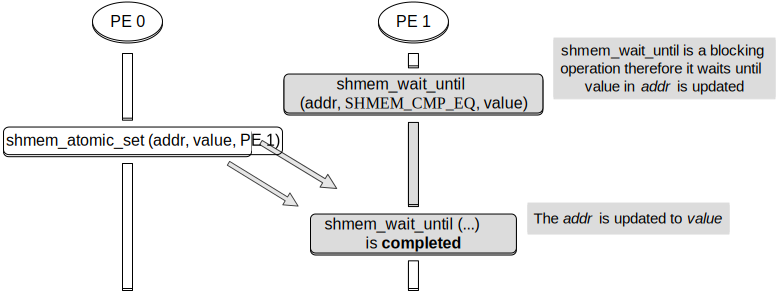
\includegraphics[width=0.7\textwidth]{figures/wait}}
\end{tabular}

\begin{tabular}{p{0.2\textwidth} | p{0.7\textwidth}}
{}
&
Waits for a symmetric variable to be updated by a remote \ac{PE}. Should be
used when computation on the local \ac{PE} cannot proceed without the value that
the remote \ac{PE} is to update. \tabularnewline
\hline 
\end{tabular}

\begin{tabular}{p{0.2\textwidth} | p{0.7\textwidth}}

{Ordering puts issued by a local \ac{PE}} \\
\FUNC{shmem\_fence} 
& 
\raisebox{-\totalheight}{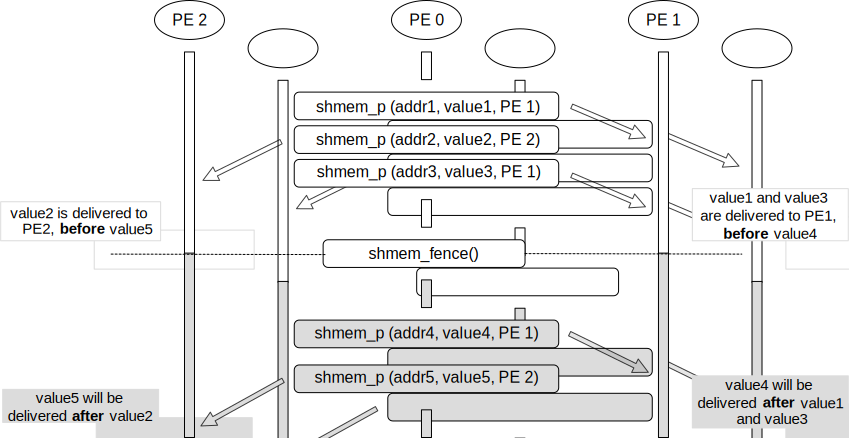
\includegraphics[width=0.7\textwidth]{figures/fence}}
\end{tabular}

\begin{tabular}{p{0.2\textwidth} | p{0.7\textwidth}}
{}
&
All \PUT{} routines, \acp{AMO} and store routines on symmetric data issued to
same \ac{PE}  are guaranteed to be delivered  before Puts (to the same \ac{PE})
issued after the \FUNC{fence} call. \tabularnewline
\hline 
\end{tabular}

\begin{tabular}{p{0.2\textwidth} | p{0.7\textwidth}}
\hline 
\textbf{\openshmem  \ac{API}} & \centering \textbf{Working of \openshmem \ac{API}} \tabularnewline
\hline 
\hline
{Ordering puts issued by all \ac{PE} }\\
\FUNC{shmem\_quiet}
& 
\raisebox{-\totalheight}{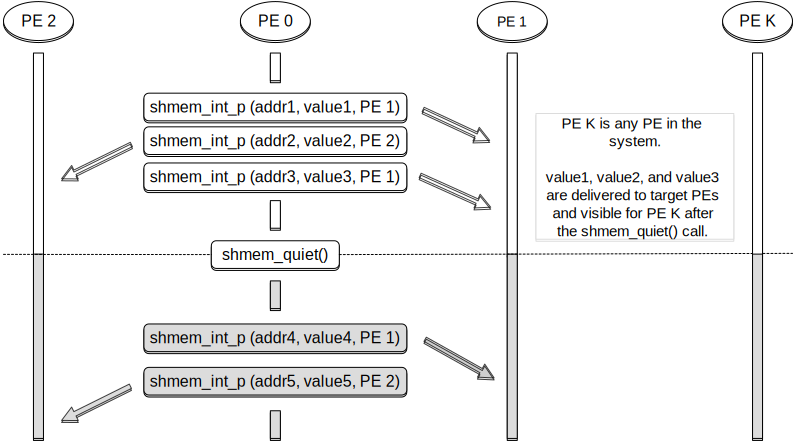
\includegraphics[width=0.7\textwidth]{figures/quiet}} 
\end{tabular}

\begin{tabular}{p{0.2\textwidth} | p{0.7\textwidth}}
{}
&
{All \PUT{} routines, \acp{AMO} and store routines on symmetric data issued by a
local \ac{PE} to all  remote \acp{PE} are guaranteed to be completed and visible
once quiet returns. This routine should be used when all remote writes issued by
a local \ac{PE} need to be visible  to all other \acp{PE} before the local
\ac{PE} proceeds. } \tabularnewline
\hline 
\end{tabular}


\begin{tabular}{p{0.2\textwidth} | p{0.7\textwidth}}
Collective synchronization over an active set \\
\FUNC{shmem\_barrier}
&  
\raisebox{-\totalheight}{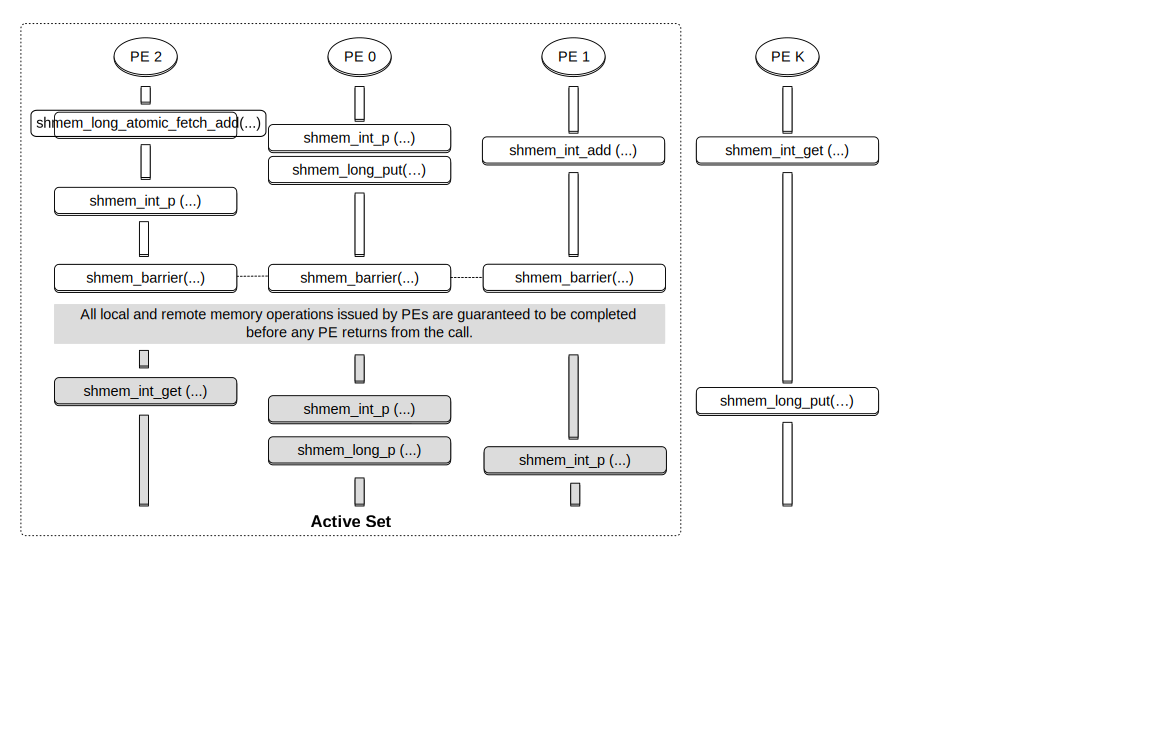
\includegraphics[width=0.7\textwidth]{figures/barrier}} 
\end{tabular}

\begin{tabular}{p{0.2\textwidth} | p{0.7\textwidth}}
{}
&
{All local and remote memory operations issued by all \acp{PE} within the
active set are guaranteed to be completed before any \ac{PE} in the
active set returns from the call. Additionally, no \ac{PE} shall return from the
barrier until all \acp{PE} in the active set have entered the same barrier
call. This routine should be used when synchronization as well as completion of
all stores and remote memory updates via \openshmem is required over a sub set
of the executing \acp{PE}.} \tabularnewline
\hline 
\end{tabular}

\begin{tabular}{p{0.2\textwidth} | p{0.7\textwidth}}
\hline 
\textbf{\openshmem  \ac{API}} & \centering \textbf{Working of \openshmem \ac{API}} \tabularnewline
\hline 
\hline
{Collective synchronization over all \acp{PE}} \\
 \FUNC{shmem\_barrier\_all}
& 
\raisebox{-\totalheight}{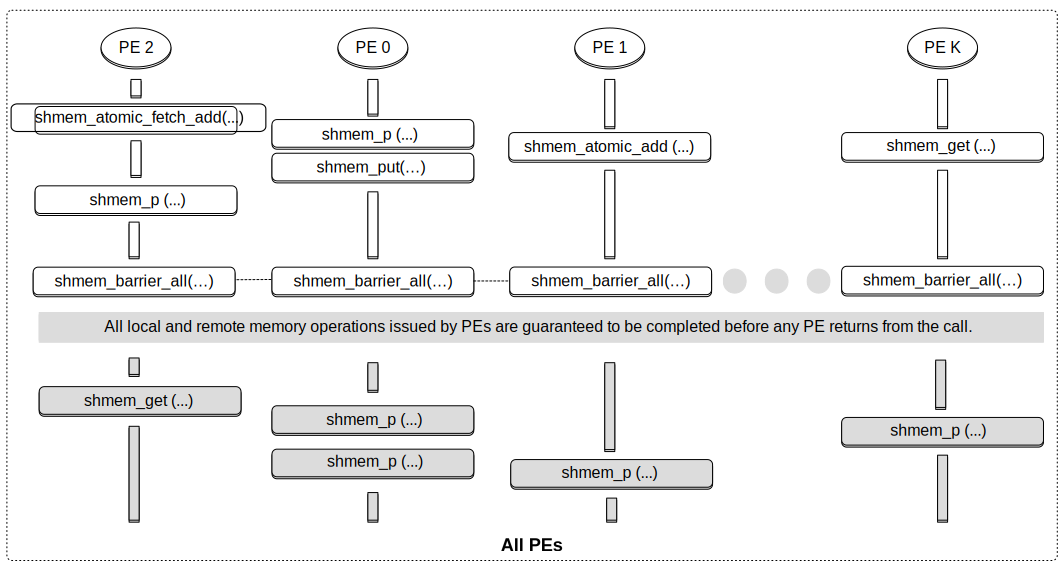
\includegraphics[width=0.7\textwidth]{figures/barrierall}}
\end{tabular}

\begin{tabular}{p{0.2\textwidth} | p{0.7\textwidth}}
{}
&
{All local and remote memory operations issued by all \acp{PE} are guaranteed to
be completed before any \ac{PE} returns from the call. Additionally no \ac{PE}
shall return from the barrier until all \acp{PE} have entered the same
\FUNC{shmem\_barrier\_all} call. This routine should be used when
synchronization as well as completion of all stores and remote memory updates
via \openshmem is required over all \acp{PE}. } \tabularnewline
\hline 
\end{tabular}
\clearpage







\subsection{Distributed Locking Routines}
The following section discusses \openshmem locks as a mechanism to provide
mutual exclusion. Three routines are available for distributed locking,
\textit{set, test} and \textit{clear}.

\subsubsection{\textbf{SHMEM\_LOCK}}\label{subsec:shmem_lock}
\apisummary{
    Releases, locks, and tests a mutual exclusion memory lock.
}
\begin{apidefinition}

\begin{Csynopsis}
void @\FuncDecl{shmem\_clear\_lock}@(long *lock);
void @\FuncDecl{shmem\_set\_lock}@(long *lock);
int @\FuncDecl{shmem\_test\_lock}@(long *lock);
\end{Csynopsis}

\begin{Fsynopsis}
INTEGER lock, SHMEM_TEST_LOCK
CALL @\FuncDecl{SHMEM\_CLEAR\_LOCK}@(lock)
CALL @\FuncDecl{SHMEM\_SET\_LOCK}@(lock)
I = @\FuncDecl{SHMEM\_TEST\_LOCK}@(lock)
\end{Fsynopsis}

\begin{apiarguments}
\apiargument{IN}{lock}{A symmetric data object that is a scalar variable or an array
    of length \CONST{1}.  This data object must be set to \CONST{0} on all
    \acp{PE} prior to the first use.  \VAR{lock} must be of type \CONST{long}.
    When using \Fortran, it must be of default kind.}
\end{apiarguments}

\apidescription{
    The \FUNC{shmem\_set\_lock} routine sets a mutual exclusion lock after
    waiting for the lock to be freed by any other \ac{PE} currently holding
    the lock.  Waiting \acp{PE} are assured of getting the lock in a
    first-come, first-served manner.  The \FUNC{shmem\_test\_lock} routine sets
    a mutual exclusion lock only if it is currently cleared.  By using this
    routine, a \ac{PE} can avoid blocking on a set lock.  If the lock is
    currently set, the routine returns without waiting.  The
    \FUNC{shmem\_clear\_lock} routine releases a lock previously set by
    \FUNC{shmem\_set\_lock} or \FUNC{shmem\_test\_lock} after performing a
    quiet operation on the default context to ensure that all symmetric memory
    accesses that occurred during the critical region are complete.  These
    routines are appropriate for protecting a critical region from simultaneous
    update by multiple \acp{PE}.

    The \openshmem lock API provides a non-reentrant mutex.  Thus, a call to
    \FUNC{shmem\_set\_lock} or \FUNC{shmem\_test\_lock} when the calling PE
    already holds the given lock will result in undefined behavior.  In a
    multithreaded \openshmem program, the user must ensure that such calls do
    not occur.
}

\apireturnvalues{
    The \FUNC{shmem\_test\_lock} routine returns \CONST{0} if the lock was
    originally cleared and this call was able to set the lock. A value of
    \CONST{1} is returned if the lock had been set and the call returned without
    waiting to set the lock.
}

\apinotes{
    The term symmetric data object is defined in Section \ref{subsec:memory_model}.
    The lock variable should always be initialized to zero and accessed only by the \openshmem locking
    \ac{API}.  Changing the value of the lock variable by other means without using
    the \openshmem \ac{API}, can lead to undefined behavior.
}

\begin{apiexamples}

\apicexample
    {The following example uses \FUNC{shmem\_lock} in a \Cstd[11] program.}
    {./example_code/shmem_lock_example.c}
    {}

\end{apiexamples}

\end{apidefinition}






\subsection{Cache Management}
All of these routines are deprecated and are provided for backwards
compatibility.  Implementations must include all items in this section, and the
routines should function properly and may notify the user about deprecation of
their use.

\subsubsection{\textbf{SHMEM\_CACHE}}\label{subsec:shmem_cache}
\apisummary{
    Controls data cache utilities. 
    (This routine is deprecated and is provided for backwards compatibility. 
    Implementations must include it, and the routines should function properly 
    while notifying the user about deprecation of its use.)
}

\begin{apidefinition}

\begin{Csynopsis}
void shmem_clear_cache_inv(void);
void shmem_set_cache_inv(void);
void shmem_clear_cache_line_inv(void *dest);
void shmem_set_cache_line_inv(void *dest);
void shmem_udcflush(void);
void shmem_udcflush_line(void *dest);
\end{Csynopsis}

\begin{Fsynopsis}
CALL SHMEM_CLEAR_CACHE_INV
CALL SHMEM_SET_CACHE_INV
CALL SHMEM_SET_CACHE_LINE_INV(dest)
CALL SHMEM_UDCFLUSH
CALL SHMEM_UDCFLUSH_LINE(dest)
\end{Fsynopsis}

\begin{apiarguments}

\apiargument{IN}{dest}{A data object that is local to the \ac{PE}.  \VAR{dest}
    can be of any noncharacter type. If you are using \Fortran, it can be of any
    kind.}

\end{apiarguments}

\apidescription{   
    \FUNC{shmem\_set\_cache\_inv} enables automatic cache coherency mode.
    
    \FUNC{shmem\_set\_cache\_line\_inv} enables automatic cache coherency mode for
    the cache line associated with the address of \VAR{dest} only.
    
    \FUNC{shmem\_clear\_cache\_inv} disables automatic cache coherency mode
    previously enabled by \FUNC{shmem\_set\_cache\ \_inv} or
    \FUNC{shmem\_set\_cache\_line\_inv}.
    
    \FUNC{shmem\_udcflush} makes the entire user data cache coherent.
    
    \FUNC{shmem\_udcflush\_line} makes coherent the cache line that corresponds with
    the address specified by \VAR{dest}.
}

\apireturnvalues{
    None.
}

\apinotes{
    These routines have been retained for improved backward compatibility with
    legacy architectures.  They are not required to be supported by implementing
    them as \VAR{no-ops} and where used, they may have no effect on cache line
    states.
}

\begin{apiexamples}

None.

\end{apiexamples}

\end{apidefinition}


\clearpage
\clearpage %%%%%%%%%%%%%%%%%%%%%%%%%%%%%%%%%%%%%%%%%%%%%%%%%%%%%%%%%%%%

\appendix

%defining pagestyle for annex
\pagestyle{fancy}
\fancyhf{}
\fancyhead[L]{\leftmark}
\fancyhead[R]{\thepage}
\renewcommand{\headrulewidth}{0pt}
\renewcommand{\thesection}{\thesectionOrig}




\chapter{Writing OpenSHMEM Programs}
\section*{Incorporating OpenSHMEM into Programs}\label{sec:writing_programs}

The following section describes how to write a ``Hello World" \openshmem program.
To write a ``Hello World" \openshmem program, the user must:

\begin{itemize}
\item Include the header file \HEADER{shmem.h} for \Cstd.
\item Add the initialization call \hyperref[subsec:shmem_init]{\FUNC{shmem\_init}}.
\item Use \openshmem calls to query the local \ac{PE} number
    (\hyperref[subsec:shmem_my_pe]{\FUNC{shmem\_my\_pe}}) and the total number
    of \acp{PE} (\hyperref[subsec:shmem_n_pes]{\FUNC{shmem\_n\_pes}}).
\item Add the finalization call \hyperref[subsec:shmem_finalize]{\FUNC{shmem\_finalize}}.
\end{itemize}

In \openshmem, the order in which lines appear in the output is not
deterministic because \acp{PE} execute asynchronously in parallel.

\SourceExample{example_code/hello-openshmem.c}{
  \label{openshmem-hello}
  ``Hello World'' example program in \Cstd
}

\ProgramOutput{example_code/hello-openshmem-c.output}{
  Possible ordering of expected output with 4 \acp{PE} from the
  program in Example~\ref{openshmem-hello}
}

\clearpage %%%%%%%%%%%%%%%%%%%%%%%%%%%%%%%%%%%%%%%%%%%%%%%%%%%%%%%%%%%%

Example~\ref{openshmem-hello-symmetric} shows a more complex
\openshmem program that illustrates the use of symmetric data objects.
Note the declaration of the \VAR{static short dest} array and its use as the
remote destination in \hyperref[subsec:shmem_put]{\FUNC{shmem\_put}}.

The \KEYWORD{static} keyword makes the \VAR{dest} array symmetric on all \acp{PE}.
Each \ac{PE} is able to transfer data to a remote \dest{} array by simply
specifying to an \openshmem routine such as \hyperref[subsec:shmem_put]{\FUNC{shmem\_put}}
the local address of the symmetric data object that will receive the data.
This local address resolution aids programmability because the address of the
\dest{} need not be exchanged with the active side (\ac{PE} \CONST{0}) prior to
the \acf{RMA} routine.

Conversely, the declaration of the \VAR{short source} array is asymmetric
(local only).
The \source{} object does not need to be symmetric because \PUT{} handles the
references to the \VAR{source} array only on the active (local) side.

\SourceExample{example_code/writing_shmem_example.c}{
  \label{openshmem-hello-symmetric}
  Example program with symmetric data objects
}

\ProgramOutput{example_code/writing_shmem_example.output}{
  Possible ordering of expected output with 4~\acp{PE} from the
  program in Example~\ref{openshmem-hello-symmetric}
}

\chapter{Compiling and Running Programs}\label{sec:compiling}
The \openshmem Specification does not specify how
\openshmem programs are compiled, linked, and run. This section shows some
examples of how wrapper programs are utilized in the \openshmem Reference
Implementation to compile and launch programs.

\section{Compilation}
\subsection*{Programs written in \Cstd}

The \openshmem Reference Implementation provides a wrapper program, named
\textbf{oshcc}, to aid in the compilation of \Cstd programs.
The wrapper may be called as follows:

\begin{lstlisting}[]
oshcc <compiler options> -o myprogram myprogram.c
\end{lstlisting}
Where the $\langle\mbox{compiler options}\rangle$ are options understood by the
underlying \Cstd compiler called by \textbf{oshcc}.


\subsection*{Programs written in \Cpp}

The \openshmem Reference Implementation provides a wrapper program, named
\textbf{oshc++}, to aid in the compilation of \Cpp programs.
The wrapper may be called as follows:

\begin{lstlisting}[]
oshc++ <compiler options> -o myprogram myprogram.cpp
\end{lstlisting}
Where the $\langle\mbox{compiler options}\rangle$ are options understood by the
underlying \Cpp compiler called by \textbf{oshc++}.


\section{Running Programs}

The \openshmem Reference Implementation provides a wrapper program, named
\textbf{oshrun}, to launch \openshmem programs.
The wrapper may be called as follows:

\begin{lstlisting}[]
oshrun <runner options> -np <#> <program> <program arguments>
\end{lstlisting}
The arguments for \textbf{oshrun} are:

\begin{tabular}{p{0.3\textwidth}p{0.6\textwidth}}
$\langle\mbox{runner options}\rangle$ & {Options passed to the underlying launcher.}\tabularnewline
-np $\langle\mbox{\#}\rangle$ & {The number of \acp{PE} to be used in the execution.}\tabularnewline
$\langle\mbox{program}\rangle$ & {The program executable to be launched.}\tabularnewline
$\langle\mbox{program arguments}\rangle$ & {Flags and other parameters to pass to the program.}\tabularnewline
\end{tabular}




\chapter{Undefined Behavior in OpenSHMEM}\label{sec:undefined}

The \openshmem Specification formalizes the expected behavior of
its library routines.  In cases where routines are improperly used
or the input is not in accordance with the Specification, the behavior
is undefined.

\begin{longtable}{|>{\raggedright}p{0.3\textwidth}|>{\raggedright}p{0.6\textwidth}|}
\hline
\textbf{Inappropriate Usage} & \textbf{Undefined Behavior}\tabularnewline
\hline
\endhead
Uninitialized library & If the \openshmem library is not initialized,
calls to \openshmem routines that do not initialize the \openshmem library have undefined
behavior.  For example, an implementation may try to continue or may abort
immediately upon an \openshmem call into the uninitialized library.
\tabularnewline
\hline
Specifying invalid \ac{PE} numbers & For \openshmem routines that accept a
\ac{PE} number as an argument, if the \ac{PE} number is invalid for the
team associated with the operation (either implicitly or explicitly), the
behavior is undefined.  An invalid \ac{PE} number includes those that are
negative or greater than or equal to the size of the associated team.
\tabularnewline
\hline
Use of non-symmetric variables & Some routines require remotely accessible
variables to perform their function.  For example, an \openshmem library may detect a \PUT{} to a non-symmetric variable
and choose to abort the program.
However, another implementation may choose to continue execution with or without a warning.
\tabularnewline
\hline
Non-symmetric allocation of symmetric memory & The symmetric memory management routines are
collectives. For example, all \acp{PE} in the program must call
\FUNC{shmem\_malloc} with the same \VAR{size} argument.  Program behavior after a
mismatched \FUNC{shmem\_malloc} call is undefined.\tabularnewline
\hline
Use of null pointers with nonzero \VAR{len} specified & In any \openshmem routine
that takes a pointer and \VAR{len} describing the number of elements in that
pointer, a null pointer may not be given unless the corresponding \VAR{len} is also
specified as zero. Otherwise, the resulting behavior is undefined.
The following cases summarize this behavior:
\begin{itemize}
    \item \VAR{len} is 0, pointer is null: supported.
    \item \VAR{len} is not 0, pointer is null: undefined behavior.
    \item \VAR{len} is 0, pointer is non-null: supported.
    \item \VAR{len} is not 0, pointer is non-null: supported.
\end{itemize}
\tabularnewline
\hline
Multithreaded use of a team in concurrent team-based collectives &
Team-based collective operations are not thread-safe on the same \VAR{team}
object.
Concurrent collective operations on the same team from multiple threads may result in undefined
behavior.
For example, it is undefined behavior for one thread to call a team-implicit
collective which implicitly operates on the world team (e.g.,
\FUNC{shmem\_barrier\_all}) and another thread to concurrently call a
team-based collective (e.g., \FUNC{shmem\_broadcastmem}) on the same world team
object, \LibHandleRef{SHMEM\_TEAM\_WORLD}. \tabularnewline
\hline
Destroying a team with unfreed private contexts & Before destroying a given
team, the user is responsible for destroying all contexts created from that team
with the \LibConstRef{SHMEM\_CTX\_PRIVATE} option enabled; otherwise, the
behavior is undefined.\tabularnewline
\hline
Creating a team with a $stride$ value equal to 0 and the $size$ value not equal to 1 &
If a $stride$ value equal to 0 is passed to \FUNC{shmem\_team\_split\_strided},
then the $size$ argument passed must be 1, or the behavior is undefined. \tabularnewline
\hline
Creating a team that implies a wrap-around sequence &
If the triplet provided to \FUNC{shmem\_team\_split\_strided} implies a
wrap-around sequence, the input is considered invalid and the behavior is
undefined.
In other words, when $stride$ is nonzero, a newly created team must only
include \acp{PE} whose subsequent parent \ac{PE} values are either all
increasing (for positive $stride$) or all decreasing (for negative
$stride$).
That is, \textit{wrap-around} with respect to the parent team's \ac{PE} values
is not permitted.
For example, the list of \acp{PE} in the parent team should not start at a high
number and then continue to include \acp{PE} in the lower end of the parent
team's \ac{PE} range. \tabularnewline
\hline
\end{longtable}


\chapter{Interoperability with Other Programming Models}\label{sec:interoperability}

OpenSHMEM routines may be used in conjunction with the routines of other
communication libraries or parallel languages in the same program. This section
describes the interoperability with other programming models, including
clarification of undefined behaviors caused by mixed use of different models,
and advice to \openshmem library users and developers that may improve the portability
and performance of hybrid programs.


\section{\ac{MPI} Interoperability}

\openshmem and \ac{MPI} are two commonly used parallel programming models for
distributed-memory systems. The user can choose to utilize both models in the same program
to efficiently and easily support various communication patterns.

A vendor may implement the \openshmem and \ac{MPI} libraries in different ways. For
instance, one may implement both \openshmem and \ac{MPI} as standalone libraries,
each of which allocates and initializes fully isolated communication
resources.
Another approach
is to implement both \openshmem and \ac{MPI} interfaces within the
same software system in order to share a communication resource when possible.

To improve interoperability and portability in \openshmem + \ac{MPI} hybrid
programming, we clarify the relevant semantics in the following subsections.


\subsection{Initialization}
In order to ensure that a hybrid program can be portably performed with different vendor
implementations, the \openshmem environment of the program must be initialized by
a call to \FUNC{shmem\_init} or \FUNC{shmem\_init\_thread} and be finalized by
a call to \FUNC{shmem\_finalize}; the \ac{MPI} environment of the program must be initialized
by a call to \FUNC{MPI\_Init} or \FUNC{MPI\_Init\_thread} and be finalized by a
call to \FUNC{MPI\_Finalize}.

\apiimpnotes{
Portable implementations of OpenSHMEM and \ac{MPI} must ensure that the initialization
calls can be made in an arbitrary order within a program; the same rule also
applies to the finalization calls. A software runtime that utilizes a shared
communication resource for \openshmem and \ac{MPI} communication may maintain an
internal reference counter in order to ensure that the shared resource is
initialized only once and thus no shared resource is released until the last
finalization call is made.
}


\subsection{Dynamic Process Creation}
\label{subsec:interoperability:mpmd}

\ac{MPI} defines a dynamic process model that allows creation of processes after
an \ac{MPI} application has started (e.g., by calling \FUNC{MPI\_Comm\_spawn}) and
connection to independent processes (e.g., through \FUNC{MPI\_Comm\_accept}
and \FUNC{MPI\_Comm\_connect}).
It provides a mechanism to establish communication
between the newly created processes and the existing \ac{MPI} application (see
\ac{MPI} standard version 3.1, Chapter 10).
Unlike \ac{MPI}, \openshmem starts all processes at once and requires all \acp{PE} to
collectively allocate and initialize resources (e.g., symmetric heap) used by
the \openshmem library before any other \openshmem routine may
be called. \openshmem does not support communication with dynamically created
or connected processes. In such a scenario, \ac{MPI} can be used to communicate
with these processes.


\subsection{Thread Safety}
\label{subsec:interoperability:thread}
Both \openshmem and \ac{MPI} define the interaction with user threads in a program
with routines that can be used for initializing and querying the thread
environment. A hybrid program may request different thread levels
at the initialization calls of \openshmem and \ac{MPI} environments; however, the
returned support level provided by the \openshmem or \ac{MPI} library might be different
from that returned in an non-hybrid program. For instance, the former
initialization call in a hybrid program may initialize a resource with the
requested thread level, but the supported level cannot be updated by a subsequent
initialization call if the underlying software runtime of \openshmem and \ac{MPI}
share the same internal communication resource.
The program should always check the \VAR{provided} thread level returned
at the corresponding initialization call or query the level of thread support
after initialization to portably ensure thread support in each communication
environment.

Both \openshmem and \ac{MPI} define similar thread levels, namely, \VAR{THREAD\_SINGLE},
\VAR{THREAD\_FUNNELED}, \VAR{THREAD\_SERIALIZED}, and \VAR{THREAD\_MULTIPLE}.
When requesting threading support in a hybrid program, however,
the following additional rules are applied if the implementations of \openshmem
and \ac{MPI} share the same internal communication resource.
It is strongly recommended to always follow these rules to ensure program
portability.

\begin{itemize}
    \item The \VAR{THREAD\_SINGLE} thread level requires a single-threaded program.
    Hence, a hybrid program should not request \VAR{THREAD\_SINGLE} at the initialization
    call of either \openshmem or \ac{MPI} but request a different thread level at the
    initialization call of the other model.

    \item The \VAR{THREAD\_FUNNELED} thread level allows only the main thread to
    make communication calls. A hybrid program using the \VAR{THREAD\_FUNNELED}
    thread level in both \openshmem and \ac{MPI} should ensure that the same main thread
    is used in both communication environments.

    \item The \VAR{THREAD\_SERIALIZED} thread level requires the program to ensure
    that communication calls are not made concurrently by multiple threads. If a
    hybrid program uses \VAR{THREAD\_SERIALIZED} in one communication environment
    and \VAR{THREAD\_SERIALIZED} or \VAR{THREAD\_FUNNELED} in the other one, it
    should also guarantee that the \openshmem and \ac{MPI} calls are not made concurrently
    from two distinct threads.
\end{itemize}

\subsection{Mapping Process Identification Numbers}
\label{subsec:interoperability:id}

Similar to the \ac{PE} number in \openshmem, \ac{MPI} defines rank as the
identification number of a process in a communicator. Both the \openshmem \ac{PE}
and the \ac{MPI} rank are unique integers assigned from zero to one less than the total
number of processes. In a hybrid program, the \openshmem
\ac{PE} number in \LibHandleRef{SHMEM\_TEAM\_WORLD}
and the \ac{MPI} rank in \VAR{MPI\_COMM\_WORLD} of a process can be equal.
This feature, however, may be provided by only some of the \openshmem and \ac{MPI}
implementations (e.g., if both environments share the same underlying process
manager) and is not portably guaranteed. A portable program should always
use the standard functions in each model, namely, \FUNC{shmem\_team\_my\_pe} in \openshmem
and \FUNC{MPI\_Comm\_rank} in \ac{MPI}, to query the process identification numbers
in each communication environment and manage the mapping of identifiers in the
program when necessary.

\subsubsection*{Examples}
\label{subsubsec:interoperability:id:example}

\SourceExample{example_code/hybrid_mpi_mapping_id.c}{
  The following example demonstrates how to manage the mapping between
  \openshmem \ac{PE} numbers and \ac{MPI} ranks in
  \VAR{MPI\_COMM\_WORLD} in a hybrid \openshmem and \ac{MPI} program.
}


\SourceExample{example_code/hybrid_mpi_mapping_id_shmem_comm.c}{
  The following example demonstrates an alternative approach for
  managing the mapping of process identification numbers in a hybrid
  program. The program creates a new MPI communicator, named
  \VAR{shmem\_comm}, that contains all processes in
  \VAR{MPI\_COMM\_WORLD} and each process has the same \ac{MPI} rank
  number as its \openshmem \ac{PE} number.
}

\subsection{RMA Programming Models}
\label{subsec:interoperability:rma}

\openshmem and \ac{MPI} each define similar one-sided communication models;
however, a portable program should not assume interoperability between these
models.
For instance, \openshmem guarantees the atomicity only of concurrent \openshmem AMO operations
that operate on symmetric data with the same datatype. Access to the same symmetric
object with \ac{MPI} atomic operations, such as an \FUNC{MPI\_Fetch\_and\_op}, may
result in an undefined result. A hybrid program should avoid situations where \ac{MPI} and
\openshmem one-sided operations perform concurrent accesses to the same memory
location; otherwise, the behavior is undefined.

\subsection{Communication Progress}
\label{subsec:interoperability:progress}

\openshmem promises the progression of communication both with and without
\openshmem calls and requires the software progress mechanism in the implementation
(e.g., a progress thread) when the hardware does not provide asynchronous communication
capabilities (see Section \ref{subsec:progress}).
In \ac{MPI}, however, a weak progress semantics is applied. That is,
an \ac{MPI} communication call is guaranteed only to complete in finite time. For
instance, an \FUNC{MPI\_Put} may be completed only when the remote process makes an \ac{MPI}
call that internally triggers the progress of \ac{MPI}, if the underlying hardware
does not support asynchronous communication. A hybrid program
should not assume that the \openshmem library also makes progress for \ac{MPI}.
It can explicitly manage the asynchronous communication of \ac{MPI} in
order to prevent any deadlock or performance degradation.


\chapter{History of OpenSHMEM}\label{sec:openshmem_history}

SHMEM has a long history as a parallel-programming model and has been
extensively used on a number of products since 1993, including the Cray T3D,
Cray X1E, Cray XT3 and XT4, \ac{SGI} Origin, \ac{SGI} Altix, Quadrics-based
clusters, and InfiniBand-based clusters.

\begin{itemize}
\item SHMEM Timeline
  \begin{itemize}
  \item Cray SHMEM
    \begin{itemize}
    \item SHMEM first introduced by Cray Research, Inc.\ in 1993 for Cray T3D
    \item Cray was acquired by \ac{SGI} in 1996
    \item Cray was acquired by Tera in 2000 (MTA)
    \item Platforms: Cray T3D, T3E, C90, J90, SV1, SV2, X1, X2, XE, XMT, XT
    \item \ac{HPE} acquired Cray in 2019
    \end{itemize}
  \item \ac{SGI} SHMEM
    \begin{itemize}
    \item \ac{SGI} acquired Cray Research, Inc.\ and SHMEM was integrated into
      \ac{SGI}'s Message Passing Toolkit (MPT)
    \item \ac{SGI} currently owns the rights to SHMEM and \openshmem
    \item Platforms: Origin, Altix 4700, Altix XE, ICE, UV
    \item \ac{SGI} was acquired by Rackable Systems in 2009
    \item \ac{SGI} and \ac{OSSS} signed a
      SHMEM trademark licensing agreement in 2010
    \item \ac{HPE} acquired \ac{SGI} in 2016
    \end{itemize}
  \end{itemize}
\end{itemize}

A listing of \openshmem implementations can be found on
\url{http://www.openshmem.org/}.








\chapter{Deprecated \acs{API}}\label{sec:dep}

\section{Overview}\label{dep:overview}
\TableIndex{Deprecated \acs{API}}
For the \openshmem Specification, deprecation is the process of identifying
\ac{API} that is supported but no longer recommended for use by users.
The deprecated \ac{API} \textbf{must} be supported until clearly
indicated as otherwise by the Specification.
This chapter records the \ac{API} or functionality that have been deprecated, the
version of the \openshmem Specification that effected the deprecation, and the
most recent version of the \openshmem Specification in which the feature was
supported before removal.

\begin{center}
\scriptsize
\begin{longtable}{|l|c|c|l|}
    \hline
    \textbf{Deprecated \ac{API}}
    & \textbf{Deprecated Since}
    & \textbf{Last Version Supported}
    & \textbf{Replaced By} \\
    \hline
    \endhead
    %% Deprecated in 1.1
    Header Directory: \hyperref[dep:mpp_header]{\HEADER{mpp}} & 1.1 & Current & (none) \\ \hline
    %% Deprecated in 1.2
    \CorCpp: \hyperref[subsec:start_pes]{\FuncRef{start\_pes}} & 1.2 & Current & \hyperref[subsec:shmem_init]{\FUNC{shmem\_init}} \\ \hline
    \Fortran: \hyperref[subsec:start_pes]{\FuncRef{START\_PES}} & 1.2 & 1.4 & \hyperref[subsec:shmem_init]{\FUNC{SHMEM\_INIT}} \\ \hline
    \hyperref[subsec:start_pes]{Implicit finalization} & 1.2 & Current & \hyperref[subsec:shmem_finalize]{\FUNC{shmem\_finalize}} \\ \hline
    \CorCpp: \FuncRef{\_my\_pe} & 1.2 & Current & \hyperref[subsec:shmem_my_pe]{\FUNC{shmem\_my\_pe}} \\ \hline
    \CorCpp: \FuncRef{\_num\_pes} & 1.2 & Current & \hyperref[subsec:shmem_n_pes]{\FUNC{shmem\_n\_pes}} \\ \hline
    \Fortran: \FuncRef{MY\_PE} & 1.2 & 1.4 & \hyperref[subsec:shmem_my_pe]{\FUNC{SHMEM\_MY\_PE}} \\ \hline
    \Fortran: \FuncRef{NUM\_PES} & 1.2 & 1.4 & \hyperref[subsec:shmem_n_pes]{\FUNC{SHMEM\_N\_PES}} \\ \hline
    \CorCpp: \FuncRef{shmalloc} & 1.2 & Current & \hyperref[sec:memory_management]{\FUNC{shmem\_malloc}} \\ \hline
    \CorCpp: \FuncRef{shfree} & 1.2 & Current & \hyperref[sec:memory_management]{\FUNC{shmem\_free}} \\ \hline
    \CorCpp: \FuncRef{shrealloc} & 1.2 & Current & \hyperref[sec:memory_management]{\FUNC{shmem\_realloc}} \\ \hline
    \CorCpp: \FuncRef{shmemalign} & 1.2 & Current & \hyperref[sec:memory_management]{\FUNC{shmem\_align}} \\ \hline
    \Fortran: \FuncRef{SHMEM\_PUT} & 1.2 & 1.4 & \hyperref[subsec:shmem_put]{\FUNC{SHMEM\_PUT8} or \FUNC{SHMEM\_PUT64}} \\ \hline
    %% Deprecated in 1.3
    \minitab{
        \CorCpp: \FuncRef{shmem\_clear\_cache\_inv}
        \\ \CorCpp: \FuncRef{shmem\_clear\_cache\_line\_inv}
        \\ \CorCpp: \FuncRef{shmem\_set\_cache\_inv}
        \\ \CorCpp: \FuncRef{shmem\_set\_cache\_line\_inv}
        \\ \CorCpp: \FuncRef{shmem\_udcflush}
        \\ \CorCpp: \FuncRef{shmem\_udcflush\_line}
        } & 1.3 & 1.4 & (none) \\ \hline
    \minitab{
        \Fortran: \FuncRef{SHMEM\_CLEAR\_CACHE\_INV}
        %% Note: At the time of deprecation, the Fortran API did not specify
        %% SHMEM_CLEAR_CACHE_LINE_INV. While this omission is certainly an error,
        %% Fortran was removed in 1.5 so the omission was never corrected.
        \\ \Fortran: \FuncRef{SHMEM\_SET\_CACHE\_INV}
        \\ \Fortran: \FuncRef{SHMEM\_SET\_CACHE\_LINE\_INV}
        \\ \Fortran: \FuncRef{SHMEM\_UDCFLUSH}
        \\ \Fortran: \FuncRef{SHMEM\_UDCFLUSH\_LINE}
        } & 1.3 & 1.4 & (none) \\ \hline
    \LibConstRef{\_SHMEM\_SYNC\_VALUE}         & 1.3 & Current & \hyperref[subsec:library_constants]{\CONST{SHMEM\_SYNC\_VALUE}} \\ \hline
    \LibConstRef{\_SHMEM\_BARRIER\_SYNC\_SIZE} & 1.3 & Current & \hyperref[subsec:library_constants]{\CONST{SHMEM\_BARRIER\_SYNC\_SIZE}} \\ \hline
    \LibConstRef{\_SHMEM\_BCAST\_SYNC\_SIZE}   & 1.3 & Current & \hyperref[subsec:library_constants]{\CONST{SHMEM\_BCAST\_SYNC\_SIZE}} \\ \hline
    \LibConstRef{\_SHMEM\_COLLECT\_SYNC\_SIZE} & 1.3 & Current & \hyperref[subsec:library_constants]{\CONST{SHMEM\_COLLECT\_SYNC\_SIZE}} \\ \hline
    \LibConstRef{\_SHMEM\_REDUCE\_SYNC\_SIZE}  & 1.3 & Current & \hyperref[subsec:library_constants]{\CONST{SHMEM\_REDUCE\_SYNC\_SIZE}} \\ \hline
    \LibConstRef{\_SHMEM\_REDUCE\_MIN\_WRKDATA\_SIZE} & 1.3 & Current & \hyperref[subsec:library_constants]{\CONST{SHMEM\_REDUCE\_MIN\_WRKDATA\_SIZE}} \\ \hline
    \LibConstRef{\_SHMEM\_MAJOR\_VERSION} & 1.3 & Current & \hyperref[subsec:library_constants]{\CONST{SHMEM\_MAJOR\_VERSION}} \\ \hline
    \LibConstRef{\_SHMEM\_MINOR\_VERSION} & 1.3 & Current & \hyperref[subsec:library_constants]{\CONST{SHMEM\_MINOR\_VERSION}} \\ \hline
    \LibConstRef{\_SHMEM\_MAX\_NAME\_LEN} & 1.3 & Current & \hyperref[subsec:library_constants]{\CONST{SHMEM\_MAX\_NAME\_LEN}} \\ \hline
    \LibConstRef{\_SHMEM\_VENDOR\_STRING} & 1.3 & Current & \hyperref[subsec:library_constants]{\CONST{SHMEM\_VENDOR\_STRING}} \\ \hline
    \LibConstRef{\_SHMEM\_CMP\_EQ} & 1.3 & Current & \hyperref[subsec:library_constants]{\CONST{SHMEM\_CMP\_EQ}} \\ \hline
    \LibConstRef{\_SHMEM\_CMP\_NE} & 1.3 & Current & \hyperref[subsec:library_constants]{\CONST{SHMEM\_CMP\_NE}} \\ \hline
    \LibConstRef{\_SHMEM\_CMP\_LT} & 1.3 & Current & \hyperref[subsec:library_constants]{\CONST{SHMEM\_CMP\_LT}} \\ \hline
    \LibConstRef{\_SHMEM\_CMP\_LE} & 1.3 & Current & \hyperref[subsec:library_constants]{\CONST{SHMEM\_CMP\_LE}} \\ \hline
    \LibConstRef{\_SHMEM\_CMP\_GT} & 1.3 & Current & \hyperref[subsec:library_constants]{\CONST{SHMEM\_CMP\_GT}} \\ \hline
    \LibConstRef{\_SHMEM\_CMP\_GE} & 1.3 & Current & \hyperref[subsec:library_constants]{\CONST{SHMEM\_CMP\_GE}} \\ \hline
    %% Deprecated in 1.4
    \EnvVarRef{SMA\_VERSION}         & 1.4 & Current & \hyperref[subsec:environment_variables]{\ENVVAR{SHMEM\_VERSION}} \\ \hline
    \EnvVarRef{SMA\_INFO}            & 1.4 & Current & \hyperref[subsec:environment_variables]{\ENVVAR{SHMEM\_INFO}} \\ \hline
    \EnvVarRef{SMA\_SYMMETRIC\_SIZE} & 1.4 & Current & \hyperref[subsec:environment_variables]{\ENVVAR{SHMEM\_SYMMETRIC\_SIZE}} \\ \hline
    \EnvVarRef{SMA\_DEBUG}           & 1.4 & Current & \hyperref[subsec:environment_variables]{\ENVVAR{SHMEM\_DEBUG}} \\ \hline
    \minitab{\CorCpp: \FuncRef{shmem\_wait}
        \\ \CorCpp: \FuncRef{shmem\_\FuncParam{TYPENAME}\_wait}}
        & 1.4 & Current & See \textbf{Notes} for \hyperref[subsec:shmem_wait_until]{\FUNC{shmem\_wait\_until}} \\ \hline
    \CorCpp: \FuncRef{shmem\_wait\_until} & 1.4 & Current
        & \Cstd[11]: \hyperref[subsec:shmem_wait_until]{\FUNC{shmem\_wait\_until}}, \CorCpp: \hyperref[subsec:shmem_wait_until]{\FUNC{shmem\_long\_wait\_until}} \\ \hline
    \minitab{\Cstd[11]: \FuncRef{shmem\_fetch}
        \\ \CorCpp: \FuncRef{shmem\_\FuncParam{TYPENAME}\_fetch}}
        & 1.4 & Current & \hyperref[subsec:shmem_atomic_fetch]{\FUNC{shmem\_atomic\_fetch}} \\ \hline
    \minitab{\Cstd[11]: \FuncRef{shmem\_set}
        \\ \CorCpp: \FuncRef{shmem\_\FuncParam{TYPENAME}\_set}}
        & 1.4 & Current & \hyperref[subsec:shmem_atomic_set]{\FUNC{shmem\_atomic\_set}} \\ \hline
    \minitab{\Cstd[11]: \FuncRef{shmem\_cswap}
        \\ \CorCpp: \FuncRef{shmem\_\FuncParam{TYPENAME}\_cswap}}
        & 1.4 & Current & \hyperref[subsec:shmem_atomic_compare_swap]{\FUNC{shmem\_atomic\_compare\_swap}} \\ \hline
    \minitab{\Cstd[11]: \FuncRef{shmem\_swap}
        \\ \CorCpp: \FuncRef{shmem\_\FuncParam{TYPENAME}\_swap}}
        & 1.4 & Current & \hyperref[subsec:shmem_atomic_swap]{\FUNC{shmem\_atomic\_swap}} \\ \hline
    \minitab{\Cstd[11]: \FuncRef{shmem\_finc}
        \\ \CorCpp: \FuncRef{shmem\_\FuncParam{TYPENAME}\_finc}}
        & 1.4 & Current & \hyperref[subsec:shmem_atomic_fetch_inc]{\FUNC{shmem\_atomic\_fetch\_inc}} \\ \hline
    \minitab{\Cstd[11]: \FuncRef{shmem\_inc}
        \\ \CorCpp: \FuncRef{shmem\_\FuncParam{TYPENAME}\_inc}}
        & 1.4 & Current & \hyperref[subsec:shmem_atomic_inc]{\FUNC{shmem\_atomic\_inc}} \\ \hline
    \minitab{\Cstd[11]: \FuncRef{shmem\_fadd}
        \\ \CorCpp: \FuncRef{shmem\_\FuncParam{TYPENAME}\_fadd}}
        & 1.4 & Current & \hyperref[subsec:shmem_atomic_fetch_add]{\FUNC{shmem\_atomic\_fetch\_add}} \\ \hline
    \minitab{\Cstd[11]: \FuncRef{shmem\_add}
        \\ \CorCpp: \FuncRef{shmem\_\FuncParam{TYPENAME}\_add}}
        & 1.4 & Current & \hyperref[subsec:shmem_atomic_add]{\FUNC{shmem\_atomic\_add}} \\ \hline
    Entire \Fortran \ac{API} & 1.4 & 1.4 & \openshmem \Cstd \ac{API} through \Fortran--\Cstd interoperability \\ \hline
    %% Deprecated in 1.5
    \minitab{
        \LibConstRef{SHMEM\_SYNC\_VALUE}
        \\ \LibConstRef{SHMEM\_SYNC\_SIZE}
        \\ \LibConstRef{SHMEM\_BARRIER\_SYNC\_SIZE}
        \\ \LibConstRef{SHMEM\_ALLTOALL\_SYNC\_SIZE}
        \\ \LibConstRef{SHMEM\_ALLTOALLS\_SYNC\_SIZE}
        \\ \LibConstRef{SHMEM\_BCAST\_SYNC\_SIZE}
        \\ \LibConstRef{SHMEM\_COLLECT\_SYNC\_SIZE}
        \\ \LibConstRef{SHMEM\_REDUCE\_SYNC\_SIZE}
        \\ \LibConstRef{SHMEM\_REDUCE\_MIN\_WRKDATA\_SIZE}
    } & 1.5 & Current & Team-based collectives, \minitab{Section~\ref{subsec:team_collectives}}. \\ \hline
    \CorCpp: Active-set-based \FuncRef{shmem\_sync}
        & 1.5 & Current & Team-based \hyperref[subsec:shmem_sync]{\FUNC{shmem\_sync}} \\ \hline
    \CorCpp: \FuncRef{shmem\_alltoall\{32, 64\}} & 1.5 & Current &
    \hyperref[subsec:shmem_alltoall]{\FUNC{shmem\_alltoall}} \\ \hline
    \CorCpp: \FuncRef{shmem\_alltoalls\{32, 64\}} & 1.5 & Current &
    \hyperref[subsec:shmem_alltoalls]{\FUNC{shmem\_alltoalls}} \\ \hline
    \CorCpp: \FuncRef{shmem\_broadcast\{32, 64\}} & 1.5 & Current &
    \hyperref[subsec:shmem_broadcast]{\FUNC{shmem\_broadcast}} \\ \hline
    \CorCpp: \FuncRef{shmem\_collect\{32, 64\}} & 1.5 & Current &
    \hyperref[subsec:shmem_collect]{\FUNC{shmem\_collect}} \\ \hline
    \CorCpp: \FuncRef{shmem\_fcollect\{32, 64\}} & 1.5 & Current &
    \hyperref[subsec:shmem_collect]{\FUNC{shmem\_fcollect}} \\ \hline
    \CorCpp: \FuncRef{shmem\_\FuncParam{TYPENAME}\_and\_to\_all}
        & 1.5 & Current & \hyperref[subsec:shmem_and_reduce]{\FUNC{shmem\_and\_reduce}} \\ \hline
    \CorCpp: \FuncRef{shmem\_\FuncParam{TYPENAME}\_or\_to\_all}
        & 1.5 & Current & \hyperref[subsec:shmem_or_reduce]{\FUNC{shmem\_or\_reduce}} \\ \hline
    \CorCpp: \FuncRef{shmem\_\FuncParam{TYPENAME}\_xor\_to\_all}
        & 1.5 & Current & \hyperref[subsec:shmem_xor_reduce]{\FUNC{shmem\_xor\_reduce}} \\ \hline
    \CorCpp: \FuncRef{shmem\_\FuncParam{TYPENAME}\_max\_to\_all}
        & 1.5 & Current & \hyperref[subsec:shmem_max_reduce]{\FUNC{shmem\_max\_reduce}} \\ \hline
    \CorCpp: \FuncRef{shmem\_\FuncParam{TYPENAME}\_min\_to\_all}
        & 1.5 & Current & \hyperref[subsec:shmem_min_reduce]{\FUNC{shmem\_min\_reduce}} \\ \hline
    \CorCpp: \FuncRef{shmem\_\FuncParam{TYPENAME}\_sum\_to\_all}
        & 1.5 & Current & \hyperref[subsec:shmem_sum_reduce]{\FUNC{shmem\_sum\_reduce}} \\ \hline
    \CorCpp: \FuncRef{shmem\_\FuncParam{TYPENAME}\_prod\_to\_all}
        & 1.5 & Current & \hyperref[subsec:shmem_prod_reduce]{\FUNC{shmem\_prod\_reduce}} \\ \hline
    \CorCpp: \hyperref[subsec:shmem_barrier]{\FuncRef{shmem\_barrier}}
        & 1.5 & Current & \hyperref[subsec:shmem_quiet]{\FuncRef{shmem\_quiet}} + \hyperref[subsec:shmem_sync]{\FuncRef{shmem\_sync}} \\ \hline
    \minitab{\Cstd[11]: \FuncRef{shmem\_wait\_until(\CTYPE{short} ...)}
        \\ \CorCpp: \FuncRef{shmem\_short\_wait\_until}}
        & 1.5 & Current & (none) \\ \hline
    \minitab{\Cstd[11]: \FuncRef{shmem\_wait\_until(\CTYPE{unsigned short} ...)}
        \\ \CorCpp: \FuncRef{shmem\_ushort\_wait\_until}}
        & 1.5 & Current & (none) \\ \hline
    \minitab{\Cstd[11]: \FuncRef{shmem\_test(\CTYPE{short} ...)}
        \\ \CorCpp: \FuncRef{shmem\_short\_test}}
        & 1.5 & Current & (none) \\ \hline
    \minitab{\Cstd[11]: \FuncRef{shmem\_test(\CTYPE{unsigned short} ...)}
        \\ \CorCpp: \FuncRef{shmem\_ushort\_test}}
        & 1.5 & Current & (none) \\ \hline
    \minitab{Table~\ref{p2psynctypes}: point-to-point synchronization types}
        & 1.5 & Current & Table~\ref{stdamotypes}: standard \ac{AMO} types \\ \hline
    %% Deprecated in 1.6
    %% Deprecated in 1.7
    %% Notes
    %% - If a hyperref spans more than one line vertically, the clickable box
    %%   will also span more than one line. To prevent this, wrap the hyperref
    %%   in a minitab. Example in 1.5: "Team-based collectives".
    \end{longtable}
\end{center}

\section{Deprecation Rationale}\label{dep:rationale}

\subsection{Header Directory: \HEADER{mpp}}
\label{dep:mpp_header}
In addition to the default system header paths, \openshmem implementations
must provide all \openshmem-specified header files from the \HEADER{mpp}
header directory such that these headers can be referenced in \CorCpp as
\begin{lstlisting}[language=]
#include <mpp/shmem.h>
#include <mpp/shmemx.h>
\end{lstlisting}
and in \Fortran as
\begin{lstlisting}[language=]
include 'mpp/shmem.fh'
include 'mpp/shmemx.fh'
\end{lstlisting}
for backwards compatibility with \ac{SGI} SHMEM.

\subsection{\CorCpp: \FUNC{start\_pes}}
\label{dep:start_pes}
The \CorCpp routine \FUNC{start\_pes} includes an unnecessary initialization
argument that is remnant of historical \emph{SHMEM} implementations and no
longer reflects the requirements of modern \openshmem implementations.
Furthermore, the naming of \FUNC{start\_pes} does not include the standardized
\shmemprefixLC{} naming prefix. This routine has been deprecated and
\openshmem users are encouraged to use \FUNC{shmem\_init} instead.

\subsection{Implicit Finalization}
Implicit finalization was deprecated and replaced with explicit finalization using the
\FUNC{shmem\_finalize} routine.  Explicit finalization improves portability and
also improves interoperability with profiling and debugging tools.

\subsection{\CorCpp: \FUNC{\_my\_pe}, \FUNC{\_num\_pes}, \FUNC{shmalloc},
    \FUNC{shfree}, \FUNC{shrealloc}, \FUNC{shmemalign}}
\label{dep:func_not_shmemunder}
The \CorCpp routines \FUNC{\_my\_pe}, \FUNC{\_num\_pes}, \FUNC{shmalloc},
\FUNC{shfree}, \FUNC{shrealloc}, and \FUNC{shmemalign} were deprecated in order
to normalize the \openshmem \ac{API} to use \shmemprefixLC{} as the standard
prefix for all routines.

\subsection{\textit{Fortran}: \FUNC{START\_PES}, \FUNC{MY\_PE}, \FUNC{NUM\_PES}} %% WARNING: Issue #66.
The \Fortran routines \FUNC{START\_PES}, \FUNC{MY\_PE}, and \FUNC{NUM\_PES}
were deprecated in order to minimize the \ac{API} differences from the deprecation
of \CorCpp routines \FUNC{start\_pes}, \FUNC{\_my\_pe}, and \FUNC{\_num\_pes}.

\subsection{\textit{Fortran}: \FUNC{SHMEM\_PUT}} %% WARNING: Issue #66.
\label{dep:fortran_shmem_put}
The \Fortran routine \FUNC{SHMEM\_PUT} is defined only for the \Fortran
\ac{API} and is semantically identical to \Fortran routines
\FUNC{SHMEM\_PUT8} and \FUNC{SHMEM\_PUT64}.  Since \FUNC{SHMEM\_PUT8} and
\FUNC{SHMEM\_PUT64} have defined equivalents in the \CorCpp interface,
\FUNC{SHMEM\_PUT} is ambiguous and has been deprecated.

\subsection{SHMEM\_CACHE}
\label{dep:shmem_cache}
The \FUNC{SHMEM\_CACHE} \ac{API}
\begin{center}
\begin{tabular}{ll}
    \CorCpp: & \Fortran: \\
    \FUNC{shmem\_clear\_cache\_inv}     & \FUNC{SHMEM\_CLEAR\_CACHE\_INV} \\
    \FUNC{shmem\_set\_cache\_inv}       & \FUNC{SHMEM\_SET\_CACHE\_INV} \\
    \FUNC{shmem\_set\_cache\_line\_inv} & \FUNC{SHMEM\_SET\_CACHE\_LINE\_INV} \\
    \FUNC{shmem\_udcflush}              & \FUNC{SHMEM\_UDCFLUSH} \\
    \FUNC{shmem\_udcflush\_line}        & \FUNC{SHMEM\_UDCFLUSH\_LINE} \\
    \FUNC{shmem\_clear\_cache\_line\_inv} \\
\end{tabular}
\end{center}
was originally implemented for systems with cache-management instructions.
This \ac{API} has largely gone unused on cache-coherent system architectures.
\FUNC{SHMEM\_CACHE} has been deprecated.

\subsection{\CONST{\_SHMEM\_*} Library Constants}
\label{dep:libconst_undershmem}
The library constants
\begin{center}
\begin{tabular}{ll}
    \CONST{\_SHMEM\_SYNC\_VALUE}         & \CONST{\_SHMEM\_MAX\_NAME\_LEN} \\
    \CONST{\_SHMEM\_BARRIER\_SYNC\_SIZE} & \CONST{\_SHMEM\_VENDOR\_STRING} \\
    \CONST{\_SHMEM\_BCAST\_SYNC\_SIZE}   & \CONST{\_SHMEM\_CMP\_EQ} \\
    \CONST{\_SHMEM\_COLLECT\_SYNC\_SIZE} & \CONST{\_SHMEM\_CMP\_NE} \\
    \CONST{\_SHMEM\_REDUCE\_SYNC\_SIZE}  & \CONST{\_SHMEM\_CMP\_LT} \\
    \CONST{\_SHMEM\_REDUCE\_MIN\_WRKDATA\_SIZE} & \CONST{\_SHMEM\_CMP\_LE} \\
    \CONST{\_SHMEM\_MAJOR\_VERSION}      & \CONST{\_SHMEM\_CMP\_GT} \\
    \CONST{\_SHMEM\_MINOR\_VERSION}      & \CONST{\_SHMEM\_CMP\_GE} \\
\end{tabular}
\end{center}
do not adhere to the \Cstd standard's reserved identifiers and the \Cpp
standard's reserved names.  These constants were deprecated and replaced
with corresponding constants of prefix \shmemprefix{} that adhere to \CorCpp{}
and \Fortran naming conventions.

\subsection{\ENVVAR{SMA\_*} Environment Variables}
\label{dep:envvar_sma}
The environment variables \ENVVAR{SMA\_VERSION}, \ENVVAR{SMA\_INFO},
\ENVVAR{SMA\_SYMMETRIC\_SIZE}, and \ENVVAR{SMA\_DEBUG}
were deprecated in order to normalize the \openshmem \ac{API} to use
\shmemprefix{} as the standard prefix for all environment variables.

\subsection{\CorCpp: \FUNC{shmem\_wait}}
\label{dep:shmem_wait}
The \CorCpp interface for \FUNC{shmem\_wait} and \FUNC{shmem\_\FuncParam{TYPENAME}\_wait}
was identified as unintuitive with respect to
the comparison operation it performed.  As \FUNC{shmem\_wait} can be trivially
replaced by \FUNC{shmem\_wait\_until} where \VAR{cmp} is
\CONST{SHMEM\_CMP\_NE}, the \FUNC{shmem\_wait} interface was deprecated in
favor of \FUNC{shmem\_wait\_until}, which makes the comparison operation
explicit and better communicates the developer's intent.

\subsection{\CorCpp: \FUNC{shmem\_wait\_until}}
\label{dep:long_typed_shmem_wait_until}
The \CTYPE{long}-typed \CorCpp routine \FUNC{shmem\_wait\_until} was deprecated
in favor of the \Cstd[11] type-generic interface of the same name or the
explicitly typed \CorCpp routine \FUNC{shmem\_long\_wait\_until}.

\subsection{\textit{C11} and \CorCpp: \FUNC{shmem\_fetch}, \FUNC{shmem\_set}, %% Issue #66.
    \FUNC{shmem\_cswap}, \FUNC{shmem\_swap}, \FUNC{shmem\_finc},
    \FUNC{shmem\_inc}, \FUNC{shmem\_fadd}, \FUNC{shmem\_add}}
\label{dep:amo_not_shmem_atomic}
The \Cstd[11] and \CorCpp interfaces for
\begin{center}
\begin{tabular}{ll}
    \Cstd[11]: & \CorCpp: \\
    \FUNC{shmem\_fetch} & \FUNC{shmem\_\FuncParam{TYPENAME}\_fetch} \\
    \FUNC{shmem\_set}   & \FUNC{shmem\_\FuncParam{TYPENAME}\_set}   \\
    \FUNC{shmem\_cswap} & \FUNC{shmem\_\FuncParam{TYPENAME}\_cswap} \\
    \FUNC{shmem\_swap}  & \FUNC{shmem\_\FuncParam{TYPENAME}\_swap}  \\
    \FUNC{shmem\_finc}  & \FUNC{shmem\_\FuncParam{TYPENAME}\_finc}  \\
    \FUNC{shmem\_inc}   & \FUNC{shmem\_\FuncParam{TYPENAME}\_inc}   \\
    \FUNC{shmem\_fadd}  & \FUNC{shmem\_\FuncParam{TYPENAME}\_fadd}  \\
    \FUNC{shmem\_add}   & \FUNC{shmem\_\FuncParam{TYPENAME}\_add}   \\
\end{tabular}
\end{center}
were deprecated and replaced with
similarly named interfaces within the \FUNC{shmem\_atomic\_*} namespace
in order to more clearly identify these calls as performing atomic operations.
In addition, the abbreviated names ``cswap'', ``finc'', and ``fadd'' were
expanded for clarity to ``compare\_swap'', ``fetch\_inc'', and ``fetch\_add''.

\subsection{\textit{Fortran} API} %% WARNING: Issue #66.
\label{dep:fortran}
The entire \openshmem \Fortran \ac{API} was deprecated in \openshmem[1.4] and
removed in \openshmem[1.5] because of a general lack of
use and a lack of conformance with legacy \Fortran standards. In lieu of an
extensive update of the \Fortran \ac{API}, \Fortran users are encouraged to
leverage the \openshmem Specification's \Cstd \ac{API} through the
\Fortran--\Cstd interoperability initially standardized by \Fortran[2003]%
\footnote{Formally, \Fortran[2003] is known as ISO/IEC~1539-1:2004(E).}.


\subsection{Active-set-based library constants and collectives}
\label{dep:active_set_libconst_and_collectives}
With the addition of \openshmem teams, Section~\ref{subsec:team}, the previous
method for performing collective
operations has been superseded by a more readable, flexible method for
organizing and communicating between groups of \acp{PE}. All collective routines
which previously indicated subgroups of \acp{PE} with a list of
parameters to describe the subgroup composition (active set) should be phased
out in favor of using collective operations with a team parameter.

The library constants
\begin{center}
\begin{tabular}{ll}
    \LibConstRef{SHMEM\_SYNC\_VALUE}            & \LibConstRef{SHMEM\_BCAST\_SYNC\_SIZE} \\
    \LibConstRef{SHMEM\_SYNC\_SIZE}             & \LibConstRef{SHMEM\_COLLECT\_SYNC\_SIZE} \\
    \LibConstRef{SHMEM\_BARRIER\_SYNC\_SIZE}    & \LibConstRef{SHMEM\_REDUCE\_SYNC\_SIZE} \\
    \LibConstRef{SHMEM\_ALLTOALL\_SYNC\_SIZE}   & \LibConstRef{SHMEM\_REDUCE\_MIN\_WRKDATA\_SIZE} \\
    \LibConstRef{SHMEM\_ALLTOALLS\_SYNC\_SIZE} \\
\end{tabular}
\end{center}
were deprecated as these constants pertain only to active-set-based collectives.

The \CorCpp active-set-based \FuncRef{shmem\_sync} routine was deprecated and
replaced with the team-based \Cstd[11] \FuncRef{shmem\_sync} or \CorCpp
\FuncRef{shmem\_team\_sync} routine.

The fixed-sized versions of the active-set-based routines
\begin{center}
\begin{tabular}{ll}
    \FuncRef{shmem\_alltoall32} & \FuncRef{shmem\_alltoall64} \\
    \FuncRef{shmem\_alltoalls32} & \FuncRef{shmem\_alltoalls64} \\
    \FuncRef{shmem\_broadcast32} & \FuncRef{shmem\_broadcast64} \\
    \FuncRef{shmem\_collect32} & \FuncRef{shmem\_collect64} \\
    \FuncRef{shmem\_fcollect32} & \FuncRef{shmem\_fcollect64} \\
\end{tabular}
\end{center}
were deprecated. Instead, all team-based collective routines use standard
\Cstd types with the option to use generic \Cstd[11] functions for more portable
and maintainable implementations.

The active-set-based reduction routines
\begin{center}
\begin{tabular}{ll}
    \FuncRef{shmem\_\FuncParam{TYPENAME}\_and\_to\_all} & \FuncRef{shmem\_\FuncParam{TYPENAME}\_max\_to\_all} \\
    \FuncRef{shmem\_\FuncParam{TYPENAME}\_or\_to\_all}  & \FuncRef{shmem\_\FuncParam{TYPENAME}\_min\_to\_all} \\
    \FuncRef{shmem\_\FuncParam{TYPENAME}\_xor\_to\_all} & \FuncRef{shmem\_\FuncParam{TYPENAME}\_sum\_to\_all} \\
                                                        & \FuncRef{shmem\_\FuncParam{TYPENAME}\_prod\_to\_all} \\
\end{tabular}
\end{center}
were deprecated and replaced with team-based reduction routines.


\subsection{\CorCpp: \FUNC{shmem\_barrier}}
\label{dep:shmem_barrier}
Each \openshmem team might
be associated with some number of communication contexts. The \FUNC{shmem\_barrier}
function implies that the default context is quiesced after synchronizing
some active set of \acp{PE}. Since teams may have some number of contexts associated
with the team, it becomes less clear which context would be the ``default'' context
for that particular team. Rather than continue to support \FUNC{shmem\_barrier}
for active-sets or teams, programs should use a call to \FUNC{shmem\_quiet}
followed by a call to \FUNC{shmem\_sync} in order to explicitly
indicate which context to quiesce.

\subsection{\textit{C11} and \CorCpp: \CTYPE{short} and \CTYPE{unsigned short} variants of \FUNC{shmem\_wait\_until} and \FUNC{shmem\_test}}
\label{dep:short_ushort_typed_shmem_wait_until_and_test}
The \CTYPE{short} and \CTYPE{unsigned short} type \CorCpp and \textit{C11}
routines for \FUNC{shmem\_wait\_until} and \FUNC{shmem\_test} were deprecated
because point-to-point synchronization routines are only compatible with
\acp{AMO} (as of \openshmem 1.5), and there is no corresponding \ac{AMO} for
\CTYPE{short} and \CTYPE{unsigned short}.

\subsection{Table~\ref{p2psynctypes}: point-to-point synchronization types}
\label{dep:p2p_sync_types}
As of \openshmem 1.5, the point-to-point synchronization routines are only
compatible with \acp{AMO}, so their interfaces are defined via the
standard \ac{AMO} types in Table~\ref{stdamotypes}.


%%
%% For section headings, use \textit{Fortran} instead of \Fortran.
%% Do not use commands that take optional arguments (e.g., \Fortran, \Cstd)
%% because they do not render at all in the PDF bookmarks.
%%
%% See Issue #66 for details.
%%


\chapter{Changes to this Document}\label{sec:changelog}

\section{Version 1.6}
\label{changelog:v1.6}
Major changes in \openshmem[1.6] include the addition of the new
\FUNC{shmem\_team\_ptr}, \FUNC{shmem\_ibget}, and \FUNC{shmem\_ibput}
functions.

The following list describes the specific changes in \openshmem[1.6]:
\begin{enumerate}
%
\item Added an inclusive (\FUNC{shmem\_sum\_inscan}) and exclusive 
(\FUNC{shmem\_sum\_exscan}) collective summation operation. 
\ChangelogRef{subsec:shmem_scan}
%
\item Added support for initialization and finalization routines to be called
    multiple times, and added an initialization status query API
    \FUNC{shmem\_query\_initialized}.
\ChangelogRef{subsec:shmem_init, subsec:shmem_finalize, subsec:shmem_query_initialized}%
%
\item Added interleaved block transfer APIs \FUNC{shmem\_ibget} and
    \FUNC{shmem\_ibput}.
\ChangelogRef{subsec:shmem_ibget, subsec:shmem_ibput}%
%
\item Added \FUNC{shmem\_signal\_add} and \FUNC{shmem\_signal\_set} to
  update a remote flag without associated data transfer of a put-with-signal operation.
\ChangelogRef{subsec:shmem_signal_add, subsec:shmem_signal_set}%
%
\item Added a team-based pointer query routine:
  \FUNC{shmem\_team\_ptr}.
\ChangelogRef{subsec:shmem_team_ptr}%
%
\item Clarified that the behavior of \FUNC{shmem\_team\_split\_strided} is
    undefined when the input \VAR{start}, \VAR{stride}, and \VAR{size} arguments
    imply a \textit{wrap-around} with respect to the parent team's \acp{PE}.
\ChangelogRef{subsec:shmem_team_split_strided}%
%
\item Added the session routines, \FUNC{shmem\_ctx\_session\_start} and
    \FUNC{shmem\_ctx\_session\_stop}, which allow users to pass hints to the
    \openshmem library to apply runtime optimizations.
\ChangelogRef{subsec:sessions}%
\item Added fine grained completion routine: \FUNC{shmem\_pe\_quiet}.
\ChangelogRef{subsec:shmem_pe_quiet}%
%
\item Split the listings for the \FUNC{shmem\_\{malloc, free, realloc, align\}}
  functions from a single entry in \openshmem[1.5] into separate entries.
\ChangelogRef{subsec:shmem_malloc, subsec:shmem_free, subsec:shmem_realloc,
  subsec:shmem_align}%
%
\item Clarified that the \FUNC{shmem\_\{malloc, free, realloc, align,
    malloc\_with\_hints, calloc\}} functions are collective operations on
    the world team.
\ChangelogRef{subsec:shmem_malloc, subsec:shmem_free, subsec:shmem_realloc,
  subsec:shmem_align, subsec:shmmallochint, subsec:shmem_calloc}%
%
\item Clarified that \FUNC{shmem\_team\_get\_config} returns the current
    configuration values, which may differ from the values assigned at the
        time of the team's creation.
\ChangelogRef{subsec:shmem_team_get_config}
%
\item Clarified the behavior of \FUNC{shmem\_team\_get\_config} when the
    \VAR{config\_mask} is 0 and/or the \VAR{config} argument is a null pointer.
\ChangelogRef{subsec:shmem_team_get_config}
%
\item Clarified the behavior of \FUNC{shmem\_team\_split\_strided} when the
    stride argument is 0 or negative.
\ChangelogRef{subsec:shmem_team_split_strided}
%
\item Clarified the requirements for the source buffer before entering the
    collective routines.
\ChangelogRef{subsec:shmem_alltoall,subsec:shmem_broadcast,subsec:shmem_collect,subsec:shmem_reductions,subsec:shmem_scan}
%
\item Added a new Errata Section~\ref{sec:errata} that indicates errors or ambiguities in the
    \openshmem specification and the version that required correction or clarification.
\ChangelogRef{sec:errata}
%
\item Removed \openshmem[1.5] Table 9, which was an incomplete duplicate of
    \openshmem[1.5] Table 10, and clarified the types, names, and supporting
    operations for team-based reductions. \label{changelog:reduction_table}
\ChangelogRef{teamreducetypes}%
%
\item Clarified that \VAR{source} and \VAR{dest} arrays must be the same
    across \acp{PE} in \openshmem reductions \label{changelog:reduction_args}
\ChangelogRef{subsec:shmem_reductions}
%
\item Clarified that \OPR{Fence} operations only guarantee ordering for
    operations that are performed on the same context. \label{changelog:fence_ctx}
\ChangelogRef{subsec:shmem_fence}%
%
\item Clarified that \FUNC{shmem\_test\_all} and \FUNC{shmem\_test\_all\_vector}
    routines return 1 when the test set is empty. \label{changelog:test_all}
\ChangelogRef{subsec:shmem_test_all,subsec:shmem_test_all_vector}%
%
\item Clarified that \FUNC{shmem\_team\_split\_strided} and
    \FUNC{shmem\_team\_split\_strided} return a nonzero value when the parent
        team compares equal to \LibConstRef{SHMEM\_TEAM\_INVALID}. \label{changelog:split_strided_2d}
\ChangelogRef{subsec:shmem_team_split_strided, subsec:shmem_team_split_2d}%
%
\item Corrected the level argument's recommended value in API notes for
    \FUNC{shmem\_pcontrol} to indicate that the value should be greater than
    2 to enable profiling with profile library defined effects and
    additional arguments. \label{changelog:pcontrol}
\ChangelogRef{subsec:shmem_pcontrol}
%
\item Added a \texttt{const} qualifier to the \VAR{cmp\_values} argument in the
    following point-to-point synchronization routines:
    \FUNC{shmem\_wait\_until\_all\_vector},
    \FUNC{shmem\_wait\_until\_any\_vector},
    \FUNC{shmem\_wait\_until\_some\_vector},
    \FUNC{shmem\_test\_all\_vector}, \FUNC{shmem\_test\_any\_vector}, and
    \FUNC{shmem\_test\_some\_vector}. \label{changelog:p2p_vector_const}
\ChangelogRef{
  subsec:shmem_wait_until_all_vector,
  subsec:shmem_wait_until_any_vector,
  subsec:shmem_wait_until_some_vector,
  subsec:shmem_test_all_vector,
  subsec:shmem_test_any_vector,
  subsec:shmem_test_some_vector}%
%

\end{enumerate}

\section{Version 1.5}
Major changes in \openshmem[1.5] include the addition of new team-based
collective functions, \OPR{put-with-signal} functions, nonblocking \ac{AMO}
functions, multiple-element point-to-point synchronization and vector
comparison functions, a \FUNC{shmem\_malloc\_with\_hints} function, a profiling
interface, and the removal of the entire \Fortran \ac{API}.

The following list describes the specific changes in \openshmem[1.5]:
\begin{enumerate}
%
\item Removed \FUNC{SHMEM\_CACHE}.
\ChangelogRef{dep:shmem_cache}%
%
\item Deprecated \CTYPE{short} and \CTYPE{unsigned short} variants for
\FUNC{shmem\_wait\_until} and \FUNC{shmem\_test}.
\ChangelogRef{
  subsec:shmem_wait_until,
  subsec:shmem_test,
  dep:short_ushort_typed_shmem_wait_until_and_test}%
%
\item Added \FUNC{shmem\_malloc\_with\_hints} interface and corresponding hints
\CONST{SHMEM\_MALLOC\_ATOMICS\_REMOTE} and \CONST{SHMEM\_MALLOC\_SIGNAL\_REMOTE}.
\ChangelogRef{subsec:shmmallochint, subsec:library_constants}%
%
\item Specified that team-based broadcast operations update the \VAR{dest} object on
all \acp{PE}, including the root \ac{PE}.
\ChangelogRef{subsec:shmem_broadcast}%
%
\item Deprecated active-set-based library constants and collective functions.
\ChangelogRef{
  subsec:library_constants,
  subsec:coll,
  dep:active_set_libconst_and_collectives,
  dep:shmem_barrier}%
%
\item Added team management functions:
  \FUNC{shmem\_team\_my\_pe},
  \FUNC{shmem\_team\_n\_pes},
  \FUNC{shmem\_team\_get\_config}, \\
  \FUNC{shmem\_team\_translate\_pe},
  \FUNC{shmem\_team\_split\_strided},
  \FUNC{shmem\_team\_split\_2d}, and
  \FUNC{shmem\_team\_destroy}.
\ChangelogRef{
  subsec:shmem_team_my_pe,
  subsec:shmem_team_n_pes,
  subsec:shmem_team_get_config,
  subsec:shmem_team_translate_pe,
  subsec:shmem_team_split_strided,
  subsec:shmem_team_split_2d,
  subsec:shmem_team_destroy}%
%
\item Added team-based communication-management functions:
  \FUNC{shmem\_team\_create\_ctx} and \\
  \FUNC{shmem\_ctx\_get\_team}.
\ChangelogRef{
  subsec:shmem_team_create_ctx,
  subsec:shmem_ctx_get_team}%
%
\item Added team-based collective functions: \FUNC{shmem\_sync},
  \FUNC{shmem\_alltoall[mem]}, \FUNC{shmem\_alltoalls[mem]}, \\
  \FUNC{shmem\_broadcast[mem]}, \FUNC{shmem\_collect[mem]}, \FUNC{shmem\_fcollect[mem]}, and \\
  \FUNC{shmem\_\{and, or, xor, max, min, sum, prod\}\_reduce}.
\ChangelogRef{
  subsec:shmem_sync,
  subsec:shmem_alltoall,
  subsec:shmem_alltoalls,
  subsec:shmem_broadcast,
  subsec:shmem_collect,
  subsec:shmem_reductions}%
%
\item Clarified interoperability of \openshmem with other programming models.
\ChangelogRef{sec:interoperability}%
%
\item Clarified restrictions on using pointers to symmetric objects.
\ChangelogRef{
  subsec:pointers_to_symmetric_objects,
  subsec:invoking_openshmem_operations}%
%
\item Added support for nonblocking \ac{AMO} functions.
\ChangelogRef{subsec:amo_nbi}%
%
\item Added support for blocking \OPR{put-with-signal} functions.
\ChangelogRef{subsec:shmem_put_signal}%
%
\item Added support for nonblocking \OPR{put-with-signal} functions.
\ChangelogRef{subsec:shmem_put_signal_nbi}%
%
\item Deprecated point-to-point synchronization types and names.
\ChangelogRef{p2psynctypes, dep:p2p_sync_types}%
%
\item Clarified that point-to-point synchronization routines preserve the
  atomicity of \openshmem \acp{AMO}.
\ChangelogRef{subsec:amo_guarantees}%
%
\item Clarified that symmetric variables used as \VAR{ivar} arguments to
  point-to-point synchronization routines must be updated using \openshmem
  \acp{AMO}.
\ChangelogRef{subsec:p2p_intro}%
%
\item Removed the entire \openshmem \Fortran \ac{API}.
\ChangelogRef{dep:fortran}%
%
\item Added support for multipliers in \VAR{SHMEM\_SYMMETRIC\_SIZE}
environment variables.
\ChangelogRef{subsec:environment_variables}%
%
\item Added support for a multiple-element point-to-point synchronization \ac{API} with
  the functions: \FUNC{shmem\_wait\_until\_all}, \FUNC{shmem\_wait\_until\_any},
  \FUNC{shmem\_wait\_until\_some}, \FUNC{shmem\_test\_all},
  \FUNC{shmem\_test\_any}, and \FUNC{shmem\_test\_some}.
\ChangelogRef{
  subsec:shmem_wait_until_all,
  subsec:shmem_wait_until_any,
  subsec:shmem_wait_until_some,
  subsec:shmem_test_all,
  subsec:shmem_test_any,
  subsec:shmem_test_some}%
%
\item Added support for vectorized comparison values in the multiple-element
  point-to-point synchronization \ac{API} with the functions:
  \FUNC{shmem\_wait\_until\_all\_vector}, \FUNC{shmem\_wait\_until\_any\_vector},
  \FUNC{shmem\_wait\_until\_some\_vector},
  \FUNC{shmem\_test\_all\_vector}, \FUNC{shmem\_test\_any\_vector}, and
  \FUNC{shmem\_test\_some\_vector}.
\ChangelogRef{
  subsec:shmem_wait_until_all_vector,
  subsec:shmem_wait_until_any_vector,
  subsec:shmem_wait_until_some_vector,
  subsec:shmem_test_all_vector,
  subsec:shmem_test_any_vector,
  subsec:shmem_test_some_vector}%
%
\item Added \openshmem profiling interface.
\ChangelogRef{sec:openshmem_profiling_interface}%
%
\item Specified the validity of communication contexts, added the constant
  \CONST{SHMEM\_CTX\_INVALID}, and clarified the behavior of
  \FUNC{shmem\_ctx\_*} routines on invalid contexts.
\ChangelogRef{sec:ctx}%
%
\item Clarified \ac{PE} active set requirements.
\ChangelogRef{subsec:coll}%
%
\item Clarified that when the \VAR{size} argument is zero, symmetric heap
    allocation routines perform no action and return a null pointer; that
    symmetric heap management routines that perform no action do not perform a
    barrier; and that the \VAR{alignment} argument to \FUNC{shmem\_align} must
    be power of two multiple of \CONST{sizeof(void*)}.
\ChangelogRef{subsec:shmem_malloc, subsec:shmem_align, subsec:shmem_realloc}%
%
\item Clarified that the \openshmem lock \ac{API} provides a non-reentrant mutex and
    that \FUNC{shmem\_clear\_lock} performs a quiet operation on the default
    context.
\ChangelogRef{subsec:shmem_lock}%
%
\item Clarified the atomicity guarantees of the \openshmem memory model.
\ChangelogRef{subsec:amo_guarantees}%
%
\end{enumerate}

\section{Version 1.4}
Major changes in \openshmem[1.4] include
multithreading support,
\emph{contexts} for communication management,
\FUNC{shmem\_sync},
\FUNC{shmem\_calloc},
expanded type support,
a new namespace for atomic operations,
atomic bitwise operations,
\FUNC{shmem\_test} for nonblocking point-to-point synchronization,
and \Cstd[11] type-generic interfaces for point-to-point synchronization.

The following list describes the specific changes in \openshmem[1.4]:
\begin{enumerate}
%
\item New communication management \ac{API}, including \FUNC{shmem\_ctx\_create};
    \FUNC{shmem\_ctx\_destroy}; and additional \ac{RMA}, \ac{AMO}, and memory ordering
    routines that accept \CTYPE{shmem\_ctx\_t} arguments.
\ChangelogRef{sec:ctx}%
%
\item New \ac{API} \FUNC{shmem\_sync\_all} and \FUNC{shmem\_sync} to provide \ac{PE}
    synchronization without completing pending communication operations.
\ChangelogRef{subsec:shmem_sync_all, subsec:shmem_sync}%
%
\item Clarified that the \openshmem extensions header files are required, even when empty.
\ChangelogRef{subsec:bindings}%
%
\item Clarified that the \FUNC{SHMEM\_GET64} and \FUNC{SHMEM\_GET64\_NBI}
    routines are included in the \Fortran language bindings.
\ChangelogRef{subsec:shmem_get, subsec:shmem_get_nbi}%
%
\item Clarified that \FUNC{shmem\_init} must be matched with a call to
    \FUNC{shmem\_finalize}.
\ChangelogRef{subsec:shmem_init, subsec:shmem_finalize}%
%
\item Added the \CONST{SHMEM\_SYNC\_SIZE} constant.
\ChangelogRef{subsec:library_constants}%
%
\item Added type-generic interfaces for \FUNC{shmem\_wait\_until}.
\ChangelogRef{subsec:shmem_wait_until}%
%
\item Removed the \VAR{volatile} qualifiers from the \VAR{ivar} arguments to
\FUNC{shmem\_wait} routines and the \VAR{lock} arguments in the lock \ac{API}.
\emph{Rationale: Volatile qualifiers were added to several \ac{API} routines in
\openshmem[1.3]; however, they were later found to be unnecessary.}
\ChangelogRef{subsec:shmem_wait_until, subsec:shmem_lock}%
%
\item Deprecated the \VAR{SMA\_}* environment variables and added equivalent
\VAR{SHMEM\_}* environment variables.
\ChangelogRef{subsec:environment_variables, dep:envvar_sma}%
%
\item Added the \Cstd[11] \CTYPE{\_Noreturn} function specifier to
\FUNC{shmem\_global\_exit}.
\ChangelogRef{subsec:shmem_global_exit}%
%
\item Clarified ordering semantics of memory ordering, point-to-point synchronization, and collective
synchronization routines.
%
\item Clarified deprecation overview and added deprecation rationale.
\ChangelogRef{dep:overview, dep:rationale}%
%
\item Deprecated header directory \HEADER{mpp}.
\ChangelogRef{dep:mpp_header}%
%
\item Deprecated the \FUNC{shmem\_wait} functions and the \CTYPE{long}-typed \CorCpp \FUNC{shmem\_wait\_until} function.
\ChangelogRef{subsec:shmem_wait_until, dep:shmem_wait, dep:long_typed_shmem_wait_until}%
%
\item Added the \FUNC{shmem\_test} functions.
\ChangelogRef{subsec:p2p_intro}%
%
\item Added the \FUNC{shmem\_calloc} function.
\ChangelogRef{subsec:shmem_calloc}%
%
\item Introduced the thread safe semantics that define the interaction between
    \openshmem routines and user threads.
\ChangelogRef{subsec:thread_support}%
%
\item Added the new routine \FUNC{shmem\_init\_thread} to initialize the
    \openshmem library with one of the defined thread levels.
\ChangelogRef{subsec:shmem_init_thread}%
%
\item Added the new routine \FUNC{shmem\_query\_thread} to query the thread
    level provided by the \openshmem implementation.
\ChangelogRef{subsec:shmem_query_thread}%
%
\item Clarified the semantics of \FUNC{shmem\_quiet} for a multithreaded
    \openshmem \ac{PE}.
\ChangelogRef{subsec:shmem_quiet}%
%
\item Revised the description of \FUNC{shmem\_barrier\_all} for a multithreaded
    \openshmem \ac{PE}.
\ChangelogRef{subsec:shmem_barrier_all}%
%
\item Revised the description of \FUNC{shmem\_wait} for a multithreaded
    \openshmem \ac{PE}.
\ChangelogRef{subsec:shmem_wait_until}%
%
\item Clarified description for \CONST{SHMEM\_VENDOR\_STRING}.
\ChangelogRef{subsec:library_constants}%
%
\item Clarified description for \CONST{SHMEM\_MAX\_NAME\_LEN}.
\ChangelogRef{subsec:library_constants}%
%
\item Clarified \ac{API} description for \FUNC{shmem\_info\_get\_name}.
\ChangelogRef{subsec:shmem_info_get_name}%
%
\item Expanded the type support for \ac{RMA}, \ac{AMO}, and point-to-point
    synchronization operations.
%% cleveref will compress a list of references by default. It is better to not
%% compress this list of *table* references because the clickable hyperref
%% links are useful. You can tell cleveref to not compress the LHS and RHS by
%% inserting an empty item between them; i.e., `,,`.
\ChangelogRef{stdrmatypes,, stdamotypes,, extamotypes,, p2psynctypes}%
%
\item Renamed \ac{AMO} operations to use \FUNC{shmem\_atomic\_*} prefix and
      deprecated old \ac{AMO} routines.
\ChangelogRef{sec:amo, dep:amo_not_shmem_atomic}%
%
\item Added fetching and non-fetching bitwise AND, OR, and XOR atomic
      operations.
\ChangelogRef{sec:amo}%
%
\item Deprecated the entire \Fortran \ac{API}.
\ChangelogRef{dep:fortran}%
%
\item Replaced the \CTYPE{complex} macro in complex-typed reductions with the
      \Cstd[99] (and later) type specifier \CTYPE{\_Complex} to remove an
      implicit dependence on \HEADER{complex.h}.
\ChangelogRef{subsec:shmem_reductions}%
%
\item Clarified that complex-typed reductions in C are optionally supported.
\ChangelogRef{subsec:shmem_reductions}%
%
\end{enumerate}




\section{Version 1.3}
Major changes in \openshmem[1.3] include the addition of
nonblocking \ac{RMA} operations,
atomic \PUT{} and \GET{} operations,
all-to-all collectives,
and \Cstd[11] type-generic interfaces for \ac{RMA} and \ac{AMO} operations.

The following list describes the specific changes in \openshmem[1.3]:
\begin{enumerate}
%
\item Clarified implementation of \acp{PE} as threads.
%
\item Added \CTYPE{const} to every read-only pointer argument.
%
\item Clarified definition of \OPR{Fence}.
\ChangelogRef{subsec:programming_model}%
%
\item Clarified implementation of symmetric memory allocation.
\ChangelogRef{subsec:memory_model}%
%
\item Restricted atomic operation guarantees to other atomic operations with the same datatype.
\ChangelogRef{subsec:amo_guarantees}%
%
\item Deprecation of all constants that start with \CONST{\_SHMEM\_*}.
\ChangelogRef{subsec:library_constants, dep:libconst_undershmem}%
%
\item Added a type-generic interface to \openshmem \ac{RMA} and \ac{AMO}
    operations based on \Cstd[11] Generics.
\ChangelogRef{sec:rma, sec:amo}%
%
\item New nonblocking variants of remote memory access, \FUNC{SHMEM\_PUT\_NBI}
    and \FUNC{SHMEM\_GET\_NBI}.
\ChangelogRef{subsec:shmem_put_nbi, subsec:shmem_get_nbi}%
%
\item New atomic elemental read and write operations, \FUNC{SHMEM\_FETCH} and
    \FUNC{SHMEM\_SET}.
\ChangelogRef{subsec:shmem_atomic_fetch, subsec:shmem_atomic_set}%
%
\item New alltoall data exchange operations, \FUNC{SHMEM\_ALLTOALL}
    and \FUNC{SHMEM\_ALLTOALLS}.
\ChangelogRef{subsec:shmem_alltoall, subsec:shmem_alltoalls}%
%
\item Added \CTYPE{volatile} to remotely accessible pointer argument in
    \FUNC{SHMEM\_WAIT} and \FUNC{SHMEM\_LOCK}.
\ChangelogRef{subsec:shmem_wait_until, subsec:shmem_lock}%
%
\item Deprecation of \FUNC{SHMEM\_CACHE}.
\ChangelogRef{dep:shmem_cache}%
%
\end{enumerate}




\section{Version 1.2}
Major changes in \openshmem[1.2] include
a new initialization routine (\FUNC{shmem\_init}),
improvements to the execution model with an explicit
library-finalization routine (\FUNC{shmem\_finalize}),
an early-exit routine (\FUNC{shmem\_global\_exit}),
namespace standardization,
and clarifications to several \ac{API} descriptions.

The following list describes the specific changes in \openshmem[1.2]:
\begin{enumerate}
%
\item Added specification of \VAR{pSync} initialization for all routines that use it.
%
\item Replaced all placeholder variable names \VAR{target} with \VAR{dest} to
      avoid confusion with \Fortran's \KEYWORD{target} keyword.
%
\item New Execution Model for exiting/finishing \openshmem programs.
\ChangelogRef{subsec:execution_model}%
%
\item New library constants to support \ac{API} that query version and name information.
\ChangelogRef{subsec:library_constants}%
%
\item New \ac{API} \FUNC{shmem\_init} to provide mechanism to start an \openshmem
      program and replace deprecated \FUNC{start\_pes}.
\ChangelogRef{subsec:shmem_init, dep:start_pes}%
%
\item Deprecation of \FUNC{\_my\_pe} and \FUNC{\_num\_pes} routines.
\ChangelogRef{subsec:shmem_my_pe, subsec:shmem_n_pes, dep:func_not_shmemunder}%
%
\item New \ac{API} \FUNC{shmem\_finalize} to provide collective mechanism to cleanly
      exit an \openshmem program and release resources.
\ChangelogRef{subsec:shmem_finalize}%
%
\item New \ac{API} \FUNC{shmem\_global\_exit} to provide mechanism to exit an
    \openshmem program.
\ChangelogRef{subsec:shmem_global_exit}%
%
\item Clarification related to the address of the referenced object in
    \FUNC{shmem\_ptr}.
\ChangelogRef{subsec:shmem_ptr}%
%
\item New \ac{API} to query the version and name information.
\ChangelogRef{subsec:shmem_info_get_version, subsec:shmem_info_get_name}%
%
\item \openshmem library \ac{API} normalization. All \Cstd symmetric memory management
      \ac{API} begins with \FUNC{shmem\_}.
\ChangelogRef{sec:memory_management, dep:func_not_shmemunder}%
%
\item Notes and clarifications added to \FUNC{shmem\_malloc}.
\ChangelogRef{subsec:shmem_malloc}%
%
\item Deprecation of \Fortran \ac{API} routine \FUNC{SHMEM\_PUT}.
\ChangelogRef{dep:fortran_shmem_put}%
See \openshmem[1.4], Section 9.5.1.
%
\item Clarification related to \FUNC{shmem\_wait}.
\ChangelogRef{subsec:shmem_wait_until}%
%
\item Undefined behavior for null pointers without zero counts added.
\ChangelogRef{sec:undefined}%
%
\item Added new Annex for clearly specifying deprecated \ac{API} and its
      support across versions of the \openshmem Specification.
\ChangelogRef{sec:dep}%
%
\end{enumerate}




\section{Version 1.1}
Major changes from \openshmem[1.0] to \openshmem[1.1] include
the introduction of the \HEADER{shmemx.h} header file for nonstandard \ac{API}
extensions,
clarifications to completion semantics and \ac{API} descriptions in agreement with
the \ac{SGI} SHMEM specification,
and general readability and usability improvements to the document structure.

The following list describes the specific changes in \openshmem[1.1]:
\begin{enumerate}
%
\item Clarifications of the completion semantics of memory synchronization
      interfaces.
\ChangelogRef{subsec:memory_order}%
%
\item Clarification of the completion semantics of memory load and store
      operations in context of \FUNC{shmem\_barrier\_all} and \FUNC{shmem\_barrier}
      routines.
\ChangelogRef{subsec:shmem_barrier_all, subsec:shmem_barrier}%
%
\item Clarification of the completion and ordering semantics of
      \FUNC{shmem\_quiet} and \FUNC{shmem\_fence}.
\ChangelogRef{subsec:shmem_quiet, subsec:shmem_fence}%
%
\item Clarifications of the completion semantics of \ac{RMA} and \ac{AMO}
      routines.
\ChangelogRef{sec:rma, sec:amo}%
%
\item Clarifications of the memory model and the memory alignment requirements
      for symmetric data objects.
\ChangelogRef{subsec:memory_model}%
%
\item Clarification of the execution model and the definition of a \ac{PE}.
\ChangelogRef{subsec:execution_model}%
%
\item Clarifications of the semantics of \FUNC{shmem\_pe\_accessible} and
      \FUNC{shmem\_addr\_accessible}.
\ChangelogRef{subsec:shmem_pe_accessible, subsec:shmem_addr_accessible}%
%
\item Added an annex on interoperability with \ac{MPI}.
\ChangelogRef{sec:interoperability}%
%
\item Added examples to the different interfaces.
%
\item Clarification of the naming conventions for constant in \Cstd and
      \Fortran.
\ChangelogRef{subsec:library_constants, subsec:shmem_wait_until}%
%
\item Added \ac{API} calls: \FUNC{shmem\_char\_p}, \FUNC{shmem\_char\_g}.
\ChangelogRef{subsec:shmem_p, subsec:shmem_g}%
%
\item Removed \ac{API} calls: \FUNC{shmem\_char\_put},
      \FUNC{shmem\_char\_get}.
\ChangelogRef{subsec:shmem_put, subsec:shmem_get}%
%
\item The usage of \CTYPE{ptrdiff\_t}, \CTYPE{size\_t}, and \CTYPE{int} in the
      interface signature was made consistent with the description.
\ChangelogRef{subsec:coll, subsec:shmem_iput, subsec:shmem_iget}%
%
\item Revised \FUNC{shmem\_barrier} example.
\ChangelogRef{subsec:shmem_barrier}%
%
\item Clarification of the initial value of \VAR{pSync} work arrays for
\FUNC{shmem\_barrier}.
\ChangelogRef{subsec:shmem_barrier}%
%
\item Clarification of the expected behavior when multiple \FUNC{start\_pes}
calls are encountered.
\ChangelogRef{subsec:start_pes}%
%
\item Corrected the definition of atomic increment operation.
\ChangelogRef{subsec:shmem_atomic_inc}%
%
\item Clarification of the size of the symmetric heap and when it is set.
\ChangelogRef{sec:memory_management}%
%
\item Clarification of the integer and real sizes for \Fortran \ac{API}.
\ChangelogRef{
  subsec:shmem_atomic_add,
  subsec:shmem_atomic_compare_swap,
  subsec:shmem_atomic_swap,
  subsec:shmem_atomic_fetch_inc,
  subsec:shmem_atomic_inc,
  subsec:shmem_atomic_fetch_add}%
%
\item Clarification of the expected behavior on program \OPR{exit}.
\ChangelogRef{subsec:execution_model}%
%
\item More detailed description for the progress of \openshmem operations
provided.
\ChangelogRef{subsec:progress}%
%
\item Clarification of naming convention for nonstandard interfaces and their
inclusion in \HEADER{shmemx.h}.
\ChangelogRef{subsec:bindings}%
%
\item Various fixes to \openshmem code examples across the Specification to
include appropriate header files.
%
\item Removing requirement that implementations should detect size mismatch and
return error information for \FUNC{shmalloc} and ensuring consistent
language.
\ChangelogRef{subsec:shmem_malloc, sec:undefined}%
%
\item \Fortran programming fixes for examples.
\ChangelogRef{subsec:shmem_reductions, subsec:shmem_wait_until}%
%
\item Clarifications of the reuse \VAR{pSync} and \VAR{pWork} across
collectives.
\ChangelogRef{
  subsec:coll,
  subsec:shmem_broadcast,
  subsec:shmem_collect,
  subsec:shmem_reductions}%
%
\item Name changes for UV and ICE for \ac{SGI} systems.
\ChangelogRef{sec:openshmem_history}%
%
\end{enumerate}

\chapter{Errata}\label{sec:errata}

Errors or ambiguities in the \openshmem specification may be discovered after
publication.
Errata, or corrections, are included in the sections below indicating the
version of the \openshmem specification that required the correction or
clarification.
These corrections have been applied to all subsequent versions of the
specification and this section serves as a historical record of the changes
made to assist users and implementors with applying the necessary corrections.
Errata that result in a change to the specification are also included in
Annex~\ref{sec:changelog}.
For an implementation to comply with a particular version of \openshmem, it
must account for all errata associated with that version as indicated below.

\section{Version 1.5}

\begin{enumerate}
  \item Removed \openshmem[1.5] Table 9, which was an incomplete duplicate of
      \openshmem[1.5] Table 10, and clarified the types, names, and supporting
      operations for team-based reductions
        (\ref{changelog:v1.6}.\ref{changelog:reduction_table}).
  \item Clarified that \VAR{source} and \VAR{dest} arrays must be the same
      across \acp{PE} in \openshmem reductions
        (\ref{changelog:v1.6}.\ref{changelog:reduction_args}).
  \item Clarified that \OPR{Fence} operations only guarantee ordering for operations
     that are performed on the same context
        (\ref{changelog:v1.6}.\ref{changelog:fence_ctx}).
  \item Clarified that \FUNC{shmem\_test\_all} and
     \FUNC{shmem\_test\_all\_vector} routines return 1 when the test set is empty
        (\ref{changelog:v1.6}.\ref{changelog:test_all}).
  \item Clarified that \FUNC{shmem\_team\_split\_strided} and
     \FUNC{shmem\_team\_split\_2d} return a nonzero value when the parent team is
     \LibConstRef{SHMEM\_TEAM\_INVALID}
        (\ref{changelog:v1.6}.\ref{changelog:split_strided_2d}).
  \item Corrected the \VAR{level} argument's recommended value in API notes for
     \FUNC{shmem\_pcontrol} to indicate that the value should be greater than 2 to enable
     profiling with profile library defined effects and additional arguments
        (\ref{changelog:v1.6}.\ref{changelog:pcontrol}).
  \item Added a \texttt{const} qualifier to the \VAR{cmp\_values} argument in the
     following point-to-point synchronization routines:
     \FUNC{shmem\_wait\_until\_all\_vector},
     \FUNC{shmem\_wait\_until\_any\_vector},
     \FUNC{shmem\_wait\_until\_some\_vector},
     \FUNC{shmem\_test\_all\_vector}, \FUNC{shmem\_test\_any\_vector}, and
     \FUNC{shmem\_test\_some\_vector}
        (\ref{changelog:v1.6}.\ref{changelog:p2p_vector_const}).
\end{enumerate}

%end of setlength command that was started in frontmatter.tex


\clearpage
\phantomsection
\addcontentsline{toc}{chapter}{Index}
\printindex

\end{document}

